\documentclass[review]{elsarticle}

\usepackage{geometry}
 \geometry{
 a4paper,
 left=30mm,
 right=30mm,
 top=10mm,
 bottom=20mm
 }

\usepackage{graphicx}
\usepackage{amsmath}

\renewcommand\thefigure{S\arabic{figure}} 
\renewcommand\thetable{S\arabic{table}} 

 \DeclareMathOperator*{\argmin}{\arg\!\min}
%% END MACROS SECTION

\usepackage{subcaption}

\usepackage{amssymb}
\usepackage{array}

\usepackage{lineno,hyperref}
\modulolinenumbers[5]

%\usepackage{numcompress}\bibliographystyle{model3-num-names}

\usepackage{natbib}
%\usepackage[numbers, sort&compress]{natbib}
%\setcitestyle{author[oxford]year}
\bibliographystyle{elsarticle-num}

%\geometry{verbose,tmargin=30mm,bmargin=25mm,lmargin=25mm,rmargin=25mm}
%\newcommand{\templatefigures}[1]
{\noindent
\begin{minipage}{2cm}
\begin{center}
%\linespread{1}
%\begin{figure}
  \centering
	\vspace{-1cm}
  
\includegraphics[height = 63px]{ISI2019only_with_date_small.pdf}\\
    %\label{matrix}
%\end{figure}
\end{center}
\end{minipage}
%
\quad
%
\begin{minipage}{12cm}
\hspace*{6.8cm}
\end{minipage}
%
\quad
%
\begin{minipage}{2cm}
\begin{center}
%\linespread{1}
\vspace{-0.9cm}

\includegraphics[scale=0.4]{imag2.jpg}\\
\end{center}

\end{minipage}

\vskip0.2cm
}


%\pagestyle{empty}
\begin{document}
%\templatefigures{}




% Model ensembles with different response variables for base and meta models:



% Spatial and Spatio-temporal Epidemiology
% Special issue: Disease Surveillance and Infectious disease Modeling


\begin{frontmatter}

\title{Supporting information: Improving disaggregation models of malaria incidence by ensembling non-linear models of prevalence}

\end{frontmatter}

\clearpage
\tableofcontents

\section{Supplementary methods}

\subsection{Extended methods for machine learning models}

We trained five machine learning models to each prevalence dataset.
These models were elastic net, projection pursuit regression,  neural networks, random forest and boosted regression trees.
All models were trained on untransformed prevalence data with any predictions below zero being set at zero.
For tree based models, transforming the data makes almost no difference.
For the other models, training on empirical logit transformed data was considered but as the final performance metric (correlation between predicted and observed polygon incidence data) was on an absolute scale it was deemed better to train the models on absolute scales.
For all models, the sample size of each survey was used as a weight.

Elastic net models are penalised, linear regression models.
They find the regression parameters that optimise
$$\hat{\beta} = \argmin_\beta \sum_{i=1}^N w_i(y_i - X_i\beta) ^ 2 + \lambda\left((1-\alpha)\beta^2 + \alpha|\beta|\right)$$
where $\beta$ is a vector of regression parameters, $y_i$ is the prevalence response data, $X_i$ is a vector of environmental covariates and $w_i$ is the weight given by the sample size. 
$\lambda$ is the penalty term and $\alpha$ controls the relative contribution of the l1 and l2 penalties.
With $\alpha = 0$ the model collapses to ridge regression while with $\alpha = 1$ the model is equivalent to the LASSO.
$\alpha$ and $\lambda$ are selected by a cross validation with candidate values given by a grid search.
We examined 15 values for $\alpha$ taken evenly between 0.05 and 1.
We examined 15 values for $\lambda$ taken as 14 values spread evenly on a log10 scale between -4 and -1 and additionally considering $\lambda = 0$ which gives the least squares estimate.

Projection pursuit regression fits a number of smooth functions to linear combinations of all the covariates. 
It involves finding regression parameters $\beta$ in the model
$$y_i = \beta_0 + \sum_{j=1}^r f_j(\beta_j X_i) $$
where the $f_j$'s are smoothing functions, $X_i$ is the vector of covariates and $r$ is the number of smooth terms to be fitted (a hyperparameter selected by cross-validation). 
The model is fitted iteratively $r$ times with the model being fitted to the residuals of the previous models at each iteration.
We considered  $r$ß in the range 1 to 15.

We fitted neural networks with a single hidden layer, logistic activation functions for the hidden units and a linear activation function for the output.
This architecture, with $h$ hidden units and $c$ covariates, can be written as
$$y_i = \beta_0 + \sum_h \beta_{ho} \operatorname{logit}^{-1}\left(\beta_{0h} + \sum_c \beta_{ih}X_{ic}\right)$$
with $\beta_0$ being the intercept, $\beta_{0h}$ being the intercept for each hidden unit, $\beta_{ih}$ being the weights between the inputs and hidden units and $\beta_{ho}$ being the weights between the hidden units and the outputs.
The nnet package optimises this model using back-propogation and includes an additional hyperparameter, 'decay', that is a penalty on the sum of the squares of the weights.
We considered a grid of hyperparameters.
For the number of hidden units we considered 15 equally spaced values between 1 and 29.
We examined 15 values for $decay$ taken as 14 values spread evenly on a log10 scale between -4 and -1 and additionally considering $\lambda = 0$.


The Random Forest algorithm creates an ensemble of regression trees.
To control overfitting each tree is fitted to a bootstrap sample of the data.
To further control overfitting, at each node of each tree, mtry random selected covariates are considered instead of the full number of covariates.
For each node in a tree the covariate and split point is found which minimises the sum of the variances in the nodes.
However, we consider two further variants of this rule.
We consider "extremely randomised trees" in which the split point for each covariate is drawn uniformly randomly.
We then consider "conditional inference trees" in which after a split point is chosen, a significance test is performed and the split point is only used if the data on each side of the split are significantly different (with a significance threshold of 0.5).
The trees are gown until all nodes reach a minimum node size.
The  split rule and the parameters mtry and the minimal node size are chosen by cross-validation.
We considered a random search of 15 parameter sets.


Finally, boosted regression trees also makes an ensemble of trees.
The trees are built sequentially and for each successive tree, the data are weighted by the size of the residual between the observed data and the prediction from all the previous trees.
The XGBoost implementation of boosted regression trees contains a number of hyperparameters: nrounds is the number of additive trees, max depth is the maximum depth of each tree, eta reduces the additional weight given to poorly predicted data points, gamma sets the minimum loss reduction needed for a split to be allowed, for each tree, a proportion colsamplebytree of covariates are considered, min child weight causes the growing of the tree to stop when a node has this many data points and finally subsample is a proportion of the data to randomly sample to use in training of each tree.
Again we used a random search and considered 15 parameter sets.

\clearpage
\section{Global dataset Machine Learning}

\clearpage
\subsection{Out-of-sample scatter plots}


\begin{figure}[h!]
  \centering
  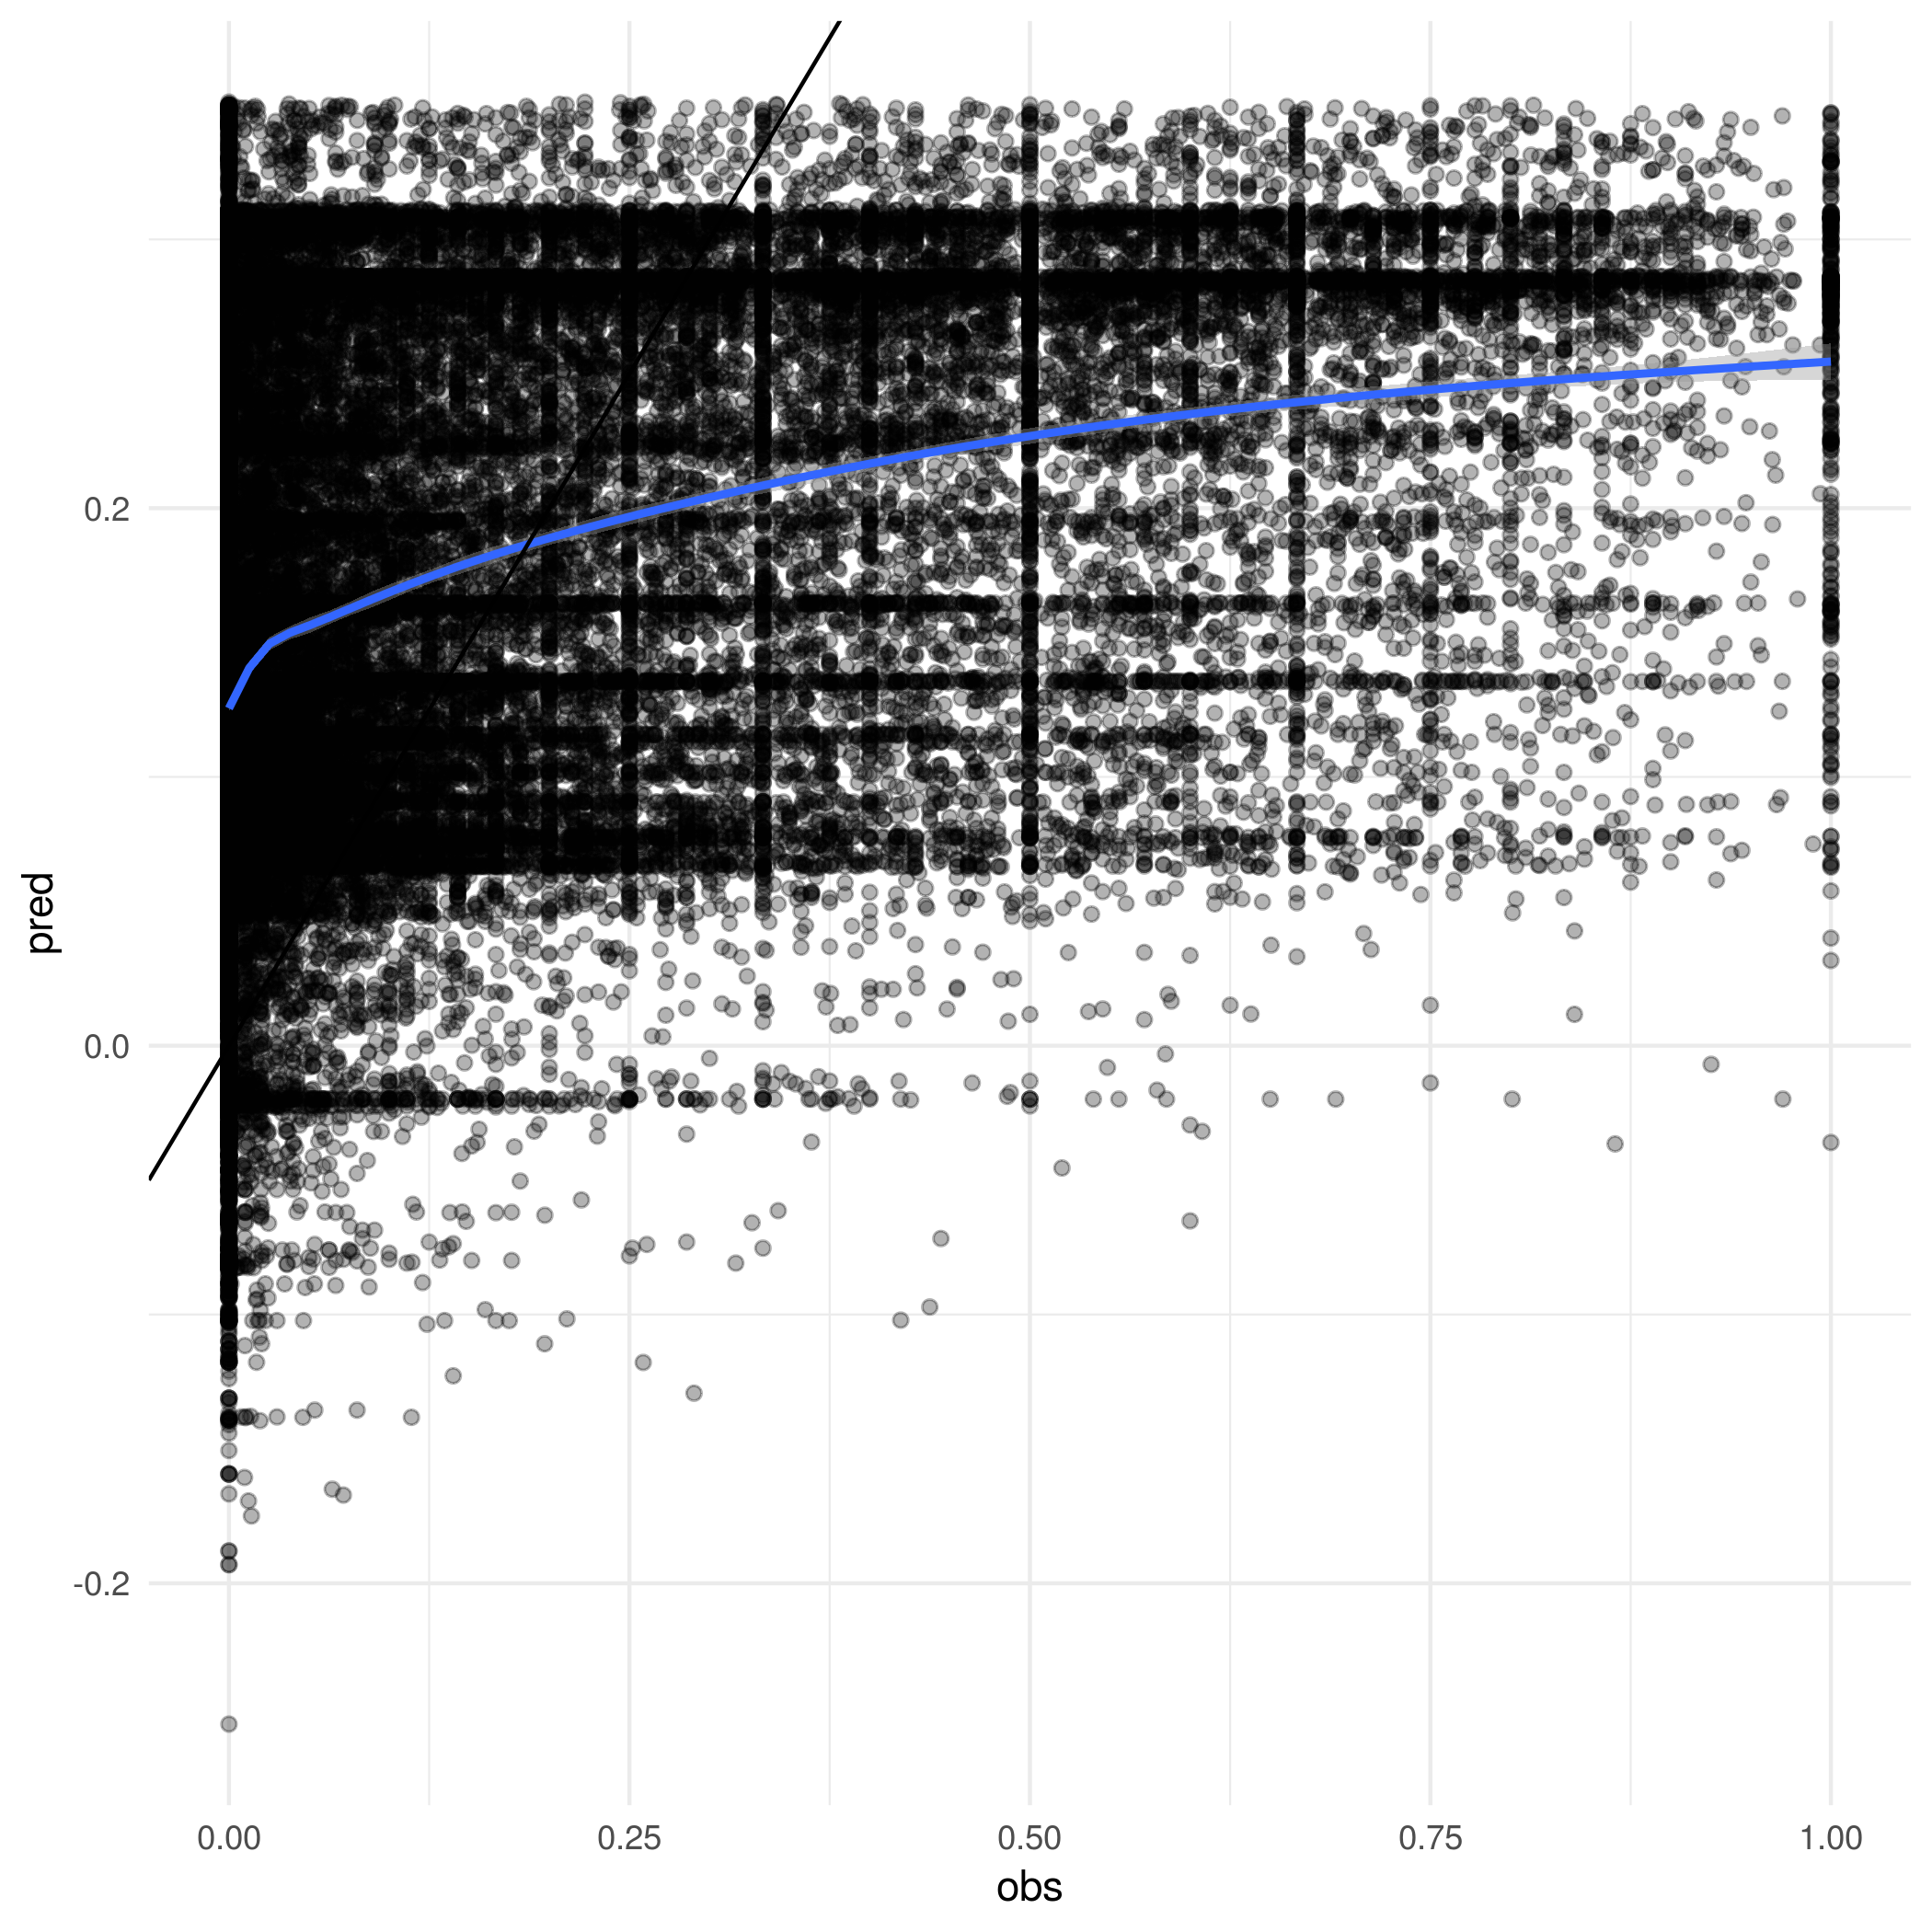
\includegraphics[width=0.6\textwidth]{figs/SI/nnet_obspred_global.png}
\caption{
  Scatter plot of predictions and held out observed data for the neural network trained on the global dataset.
}

\end{figure}



\begin{figure}[h!]
  \centering
  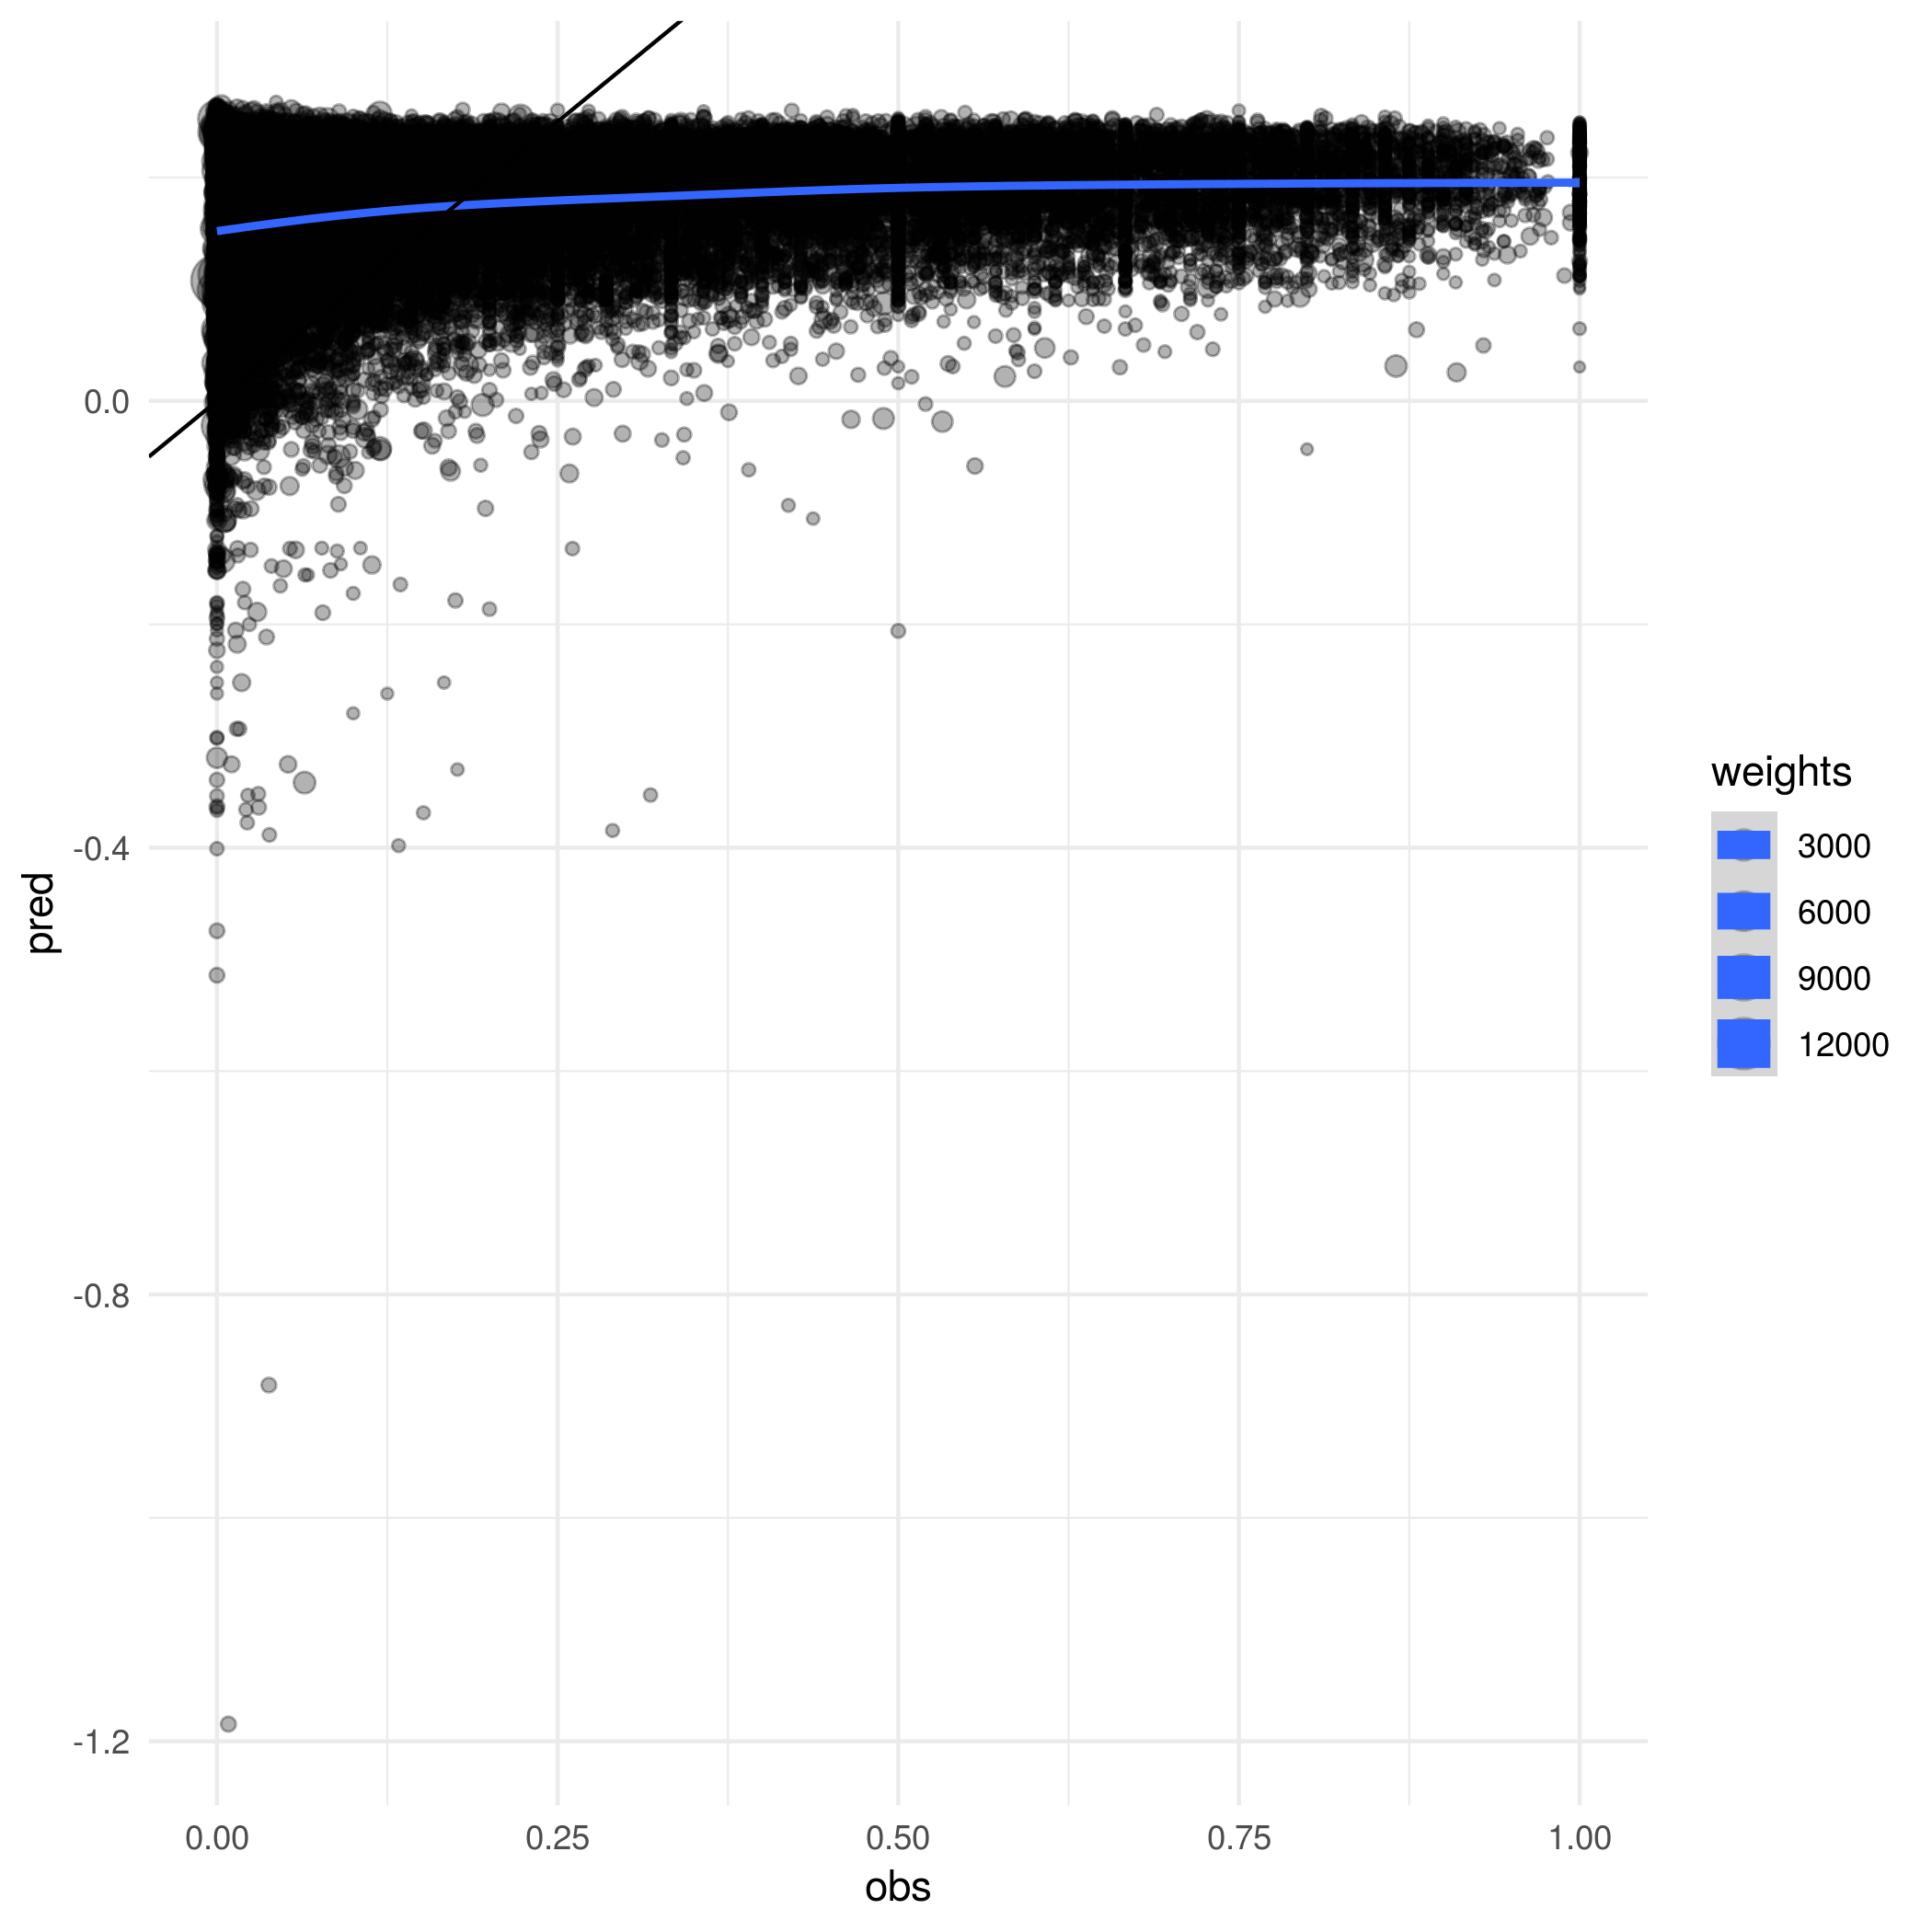
\includegraphics[width=0.6\textwidth]{figs/SI/enet_obspred_global.png}
\caption{
  Scatter plot of predictions and held out observed data for the elastic net trained on the global dataset.
}

\end{figure}


\begin{figure}[h!]
  \centering
  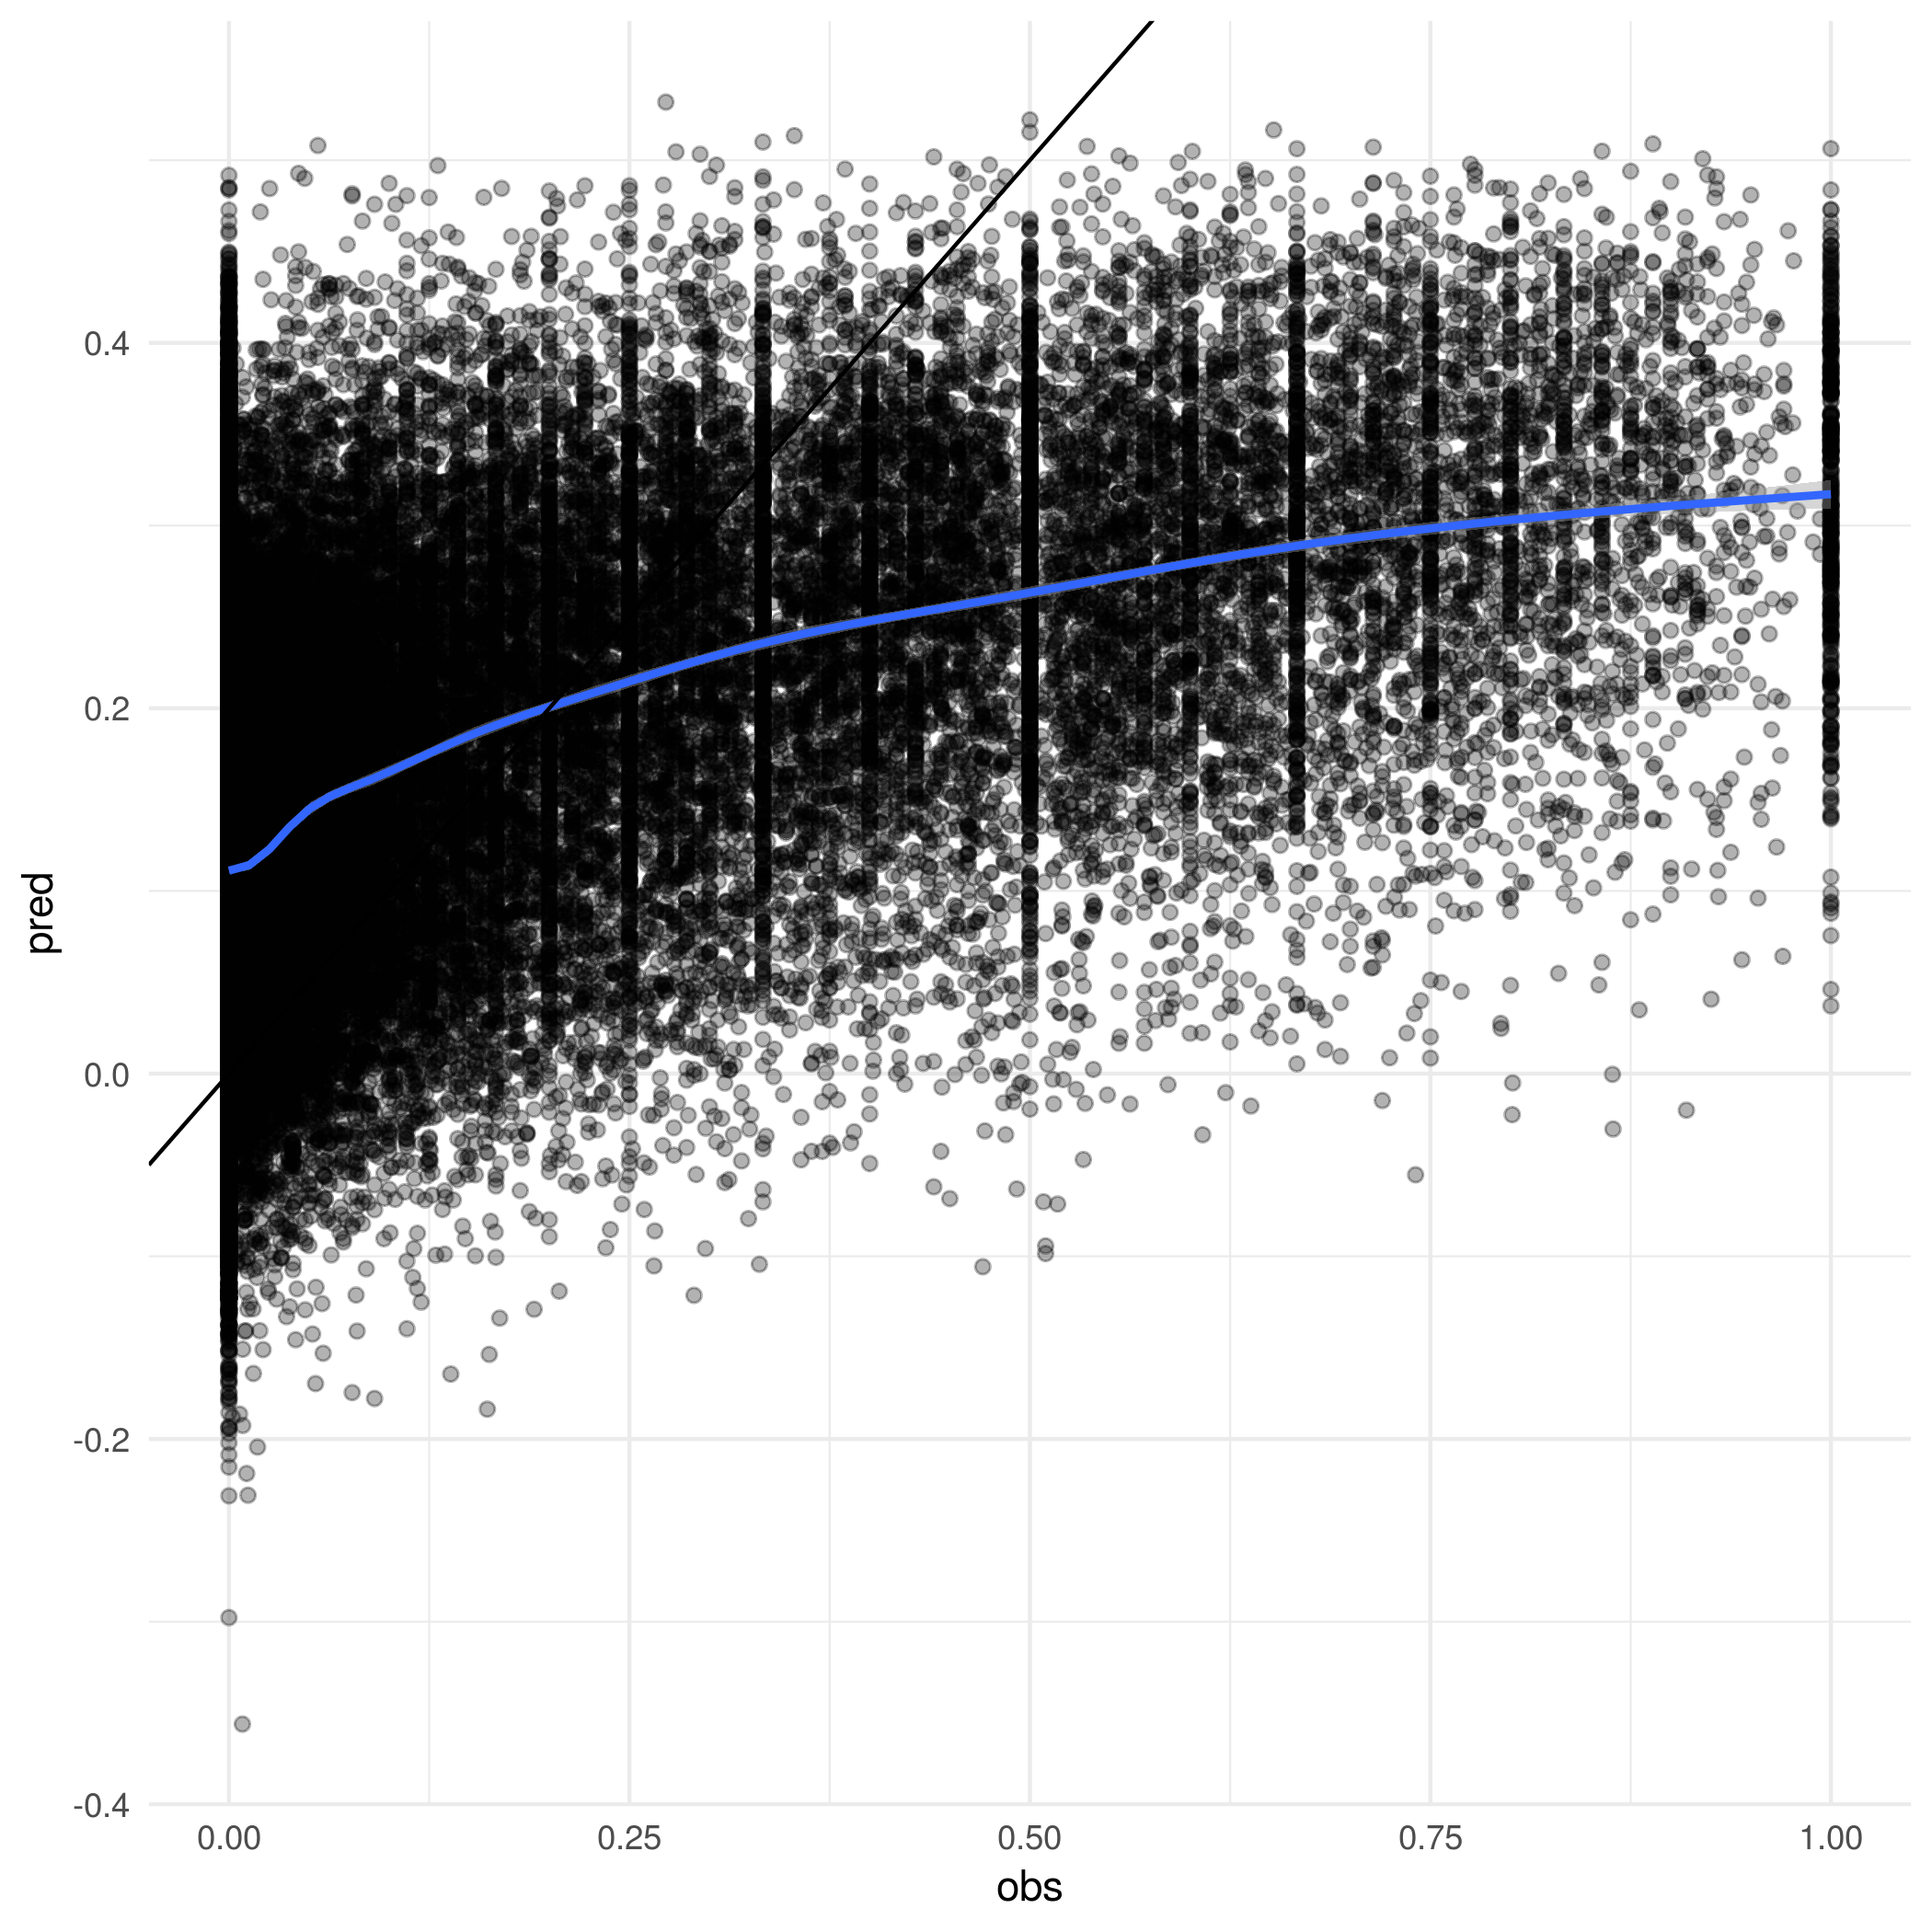
\includegraphics[width=0.6\textwidth]{figs/SI/ppr_obspred_global.png}
\caption{
  Scatter plot of predictions and held out observed data for the PPR trained on the global dataset.
}

\end{figure}


\begin{figure}[h!]
  \centering
  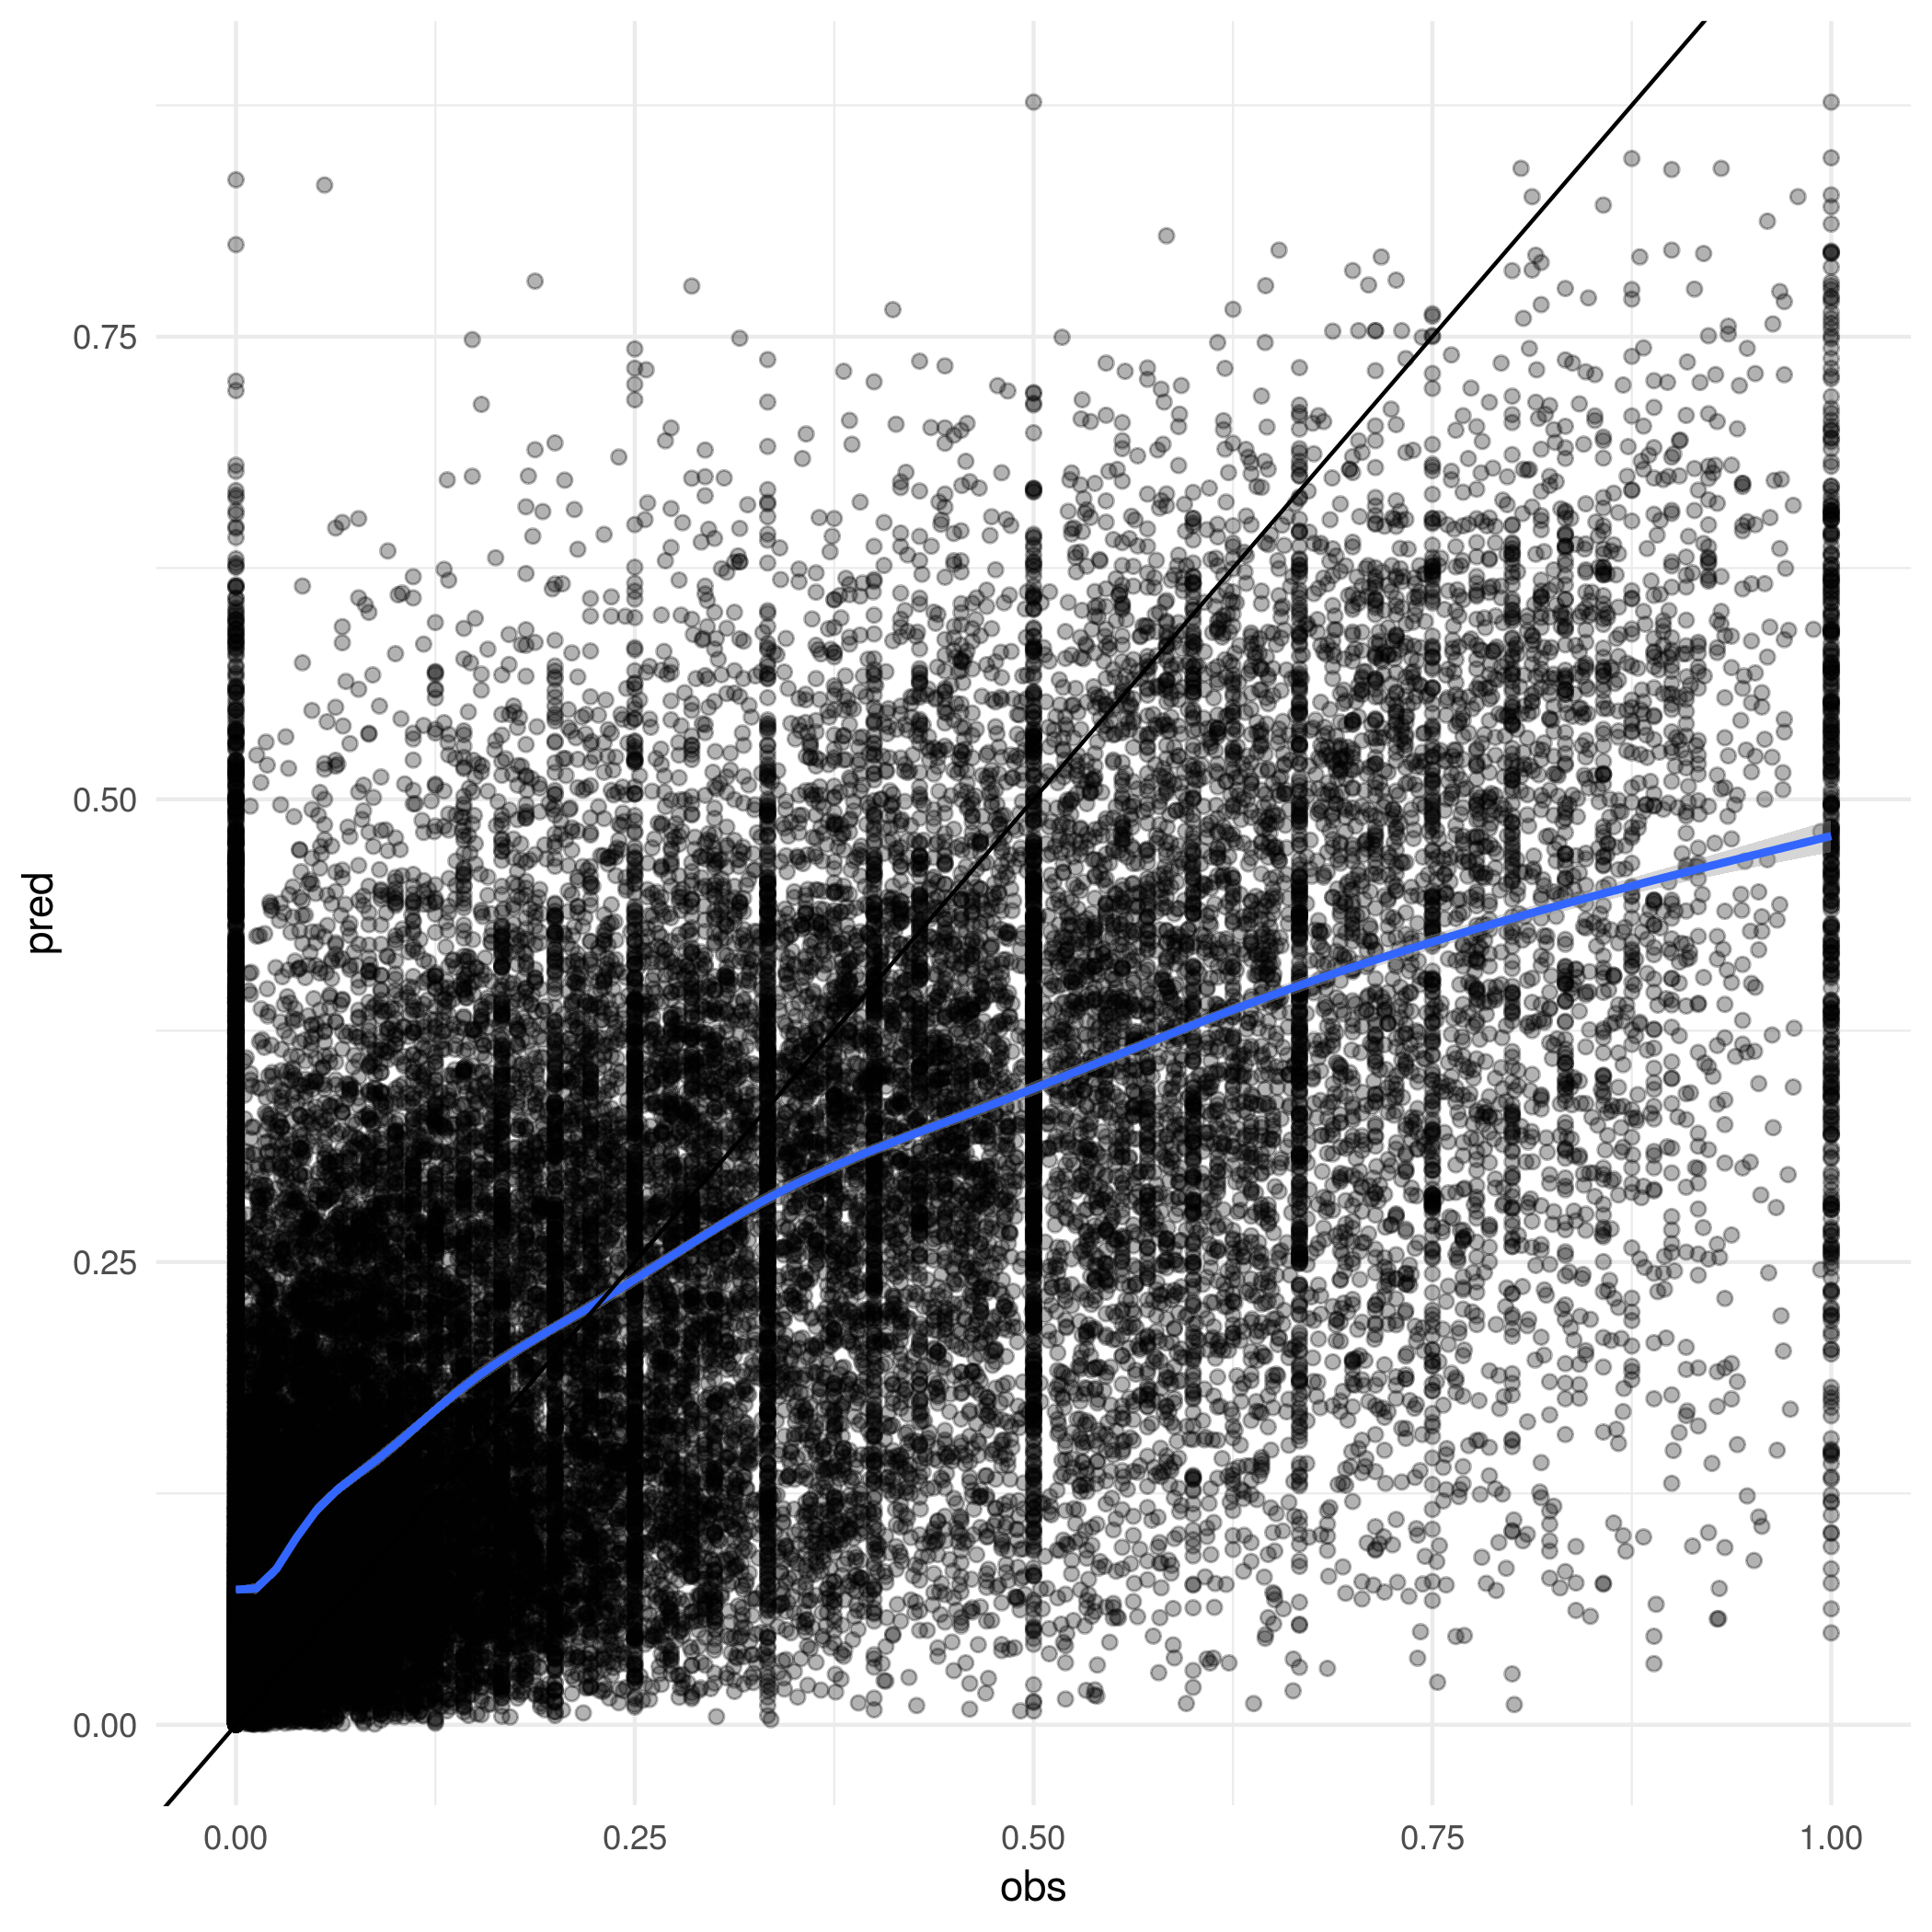
\includegraphics[width=0.6\textwidth]{figs/SI/ranger_obspred_global.png}
\caption{
  Scatter plot of predictions and held out observed data for the Random Forest trained on the global dataset.
}

\end{figure}


\begin{figure}[h!]
  \centering
  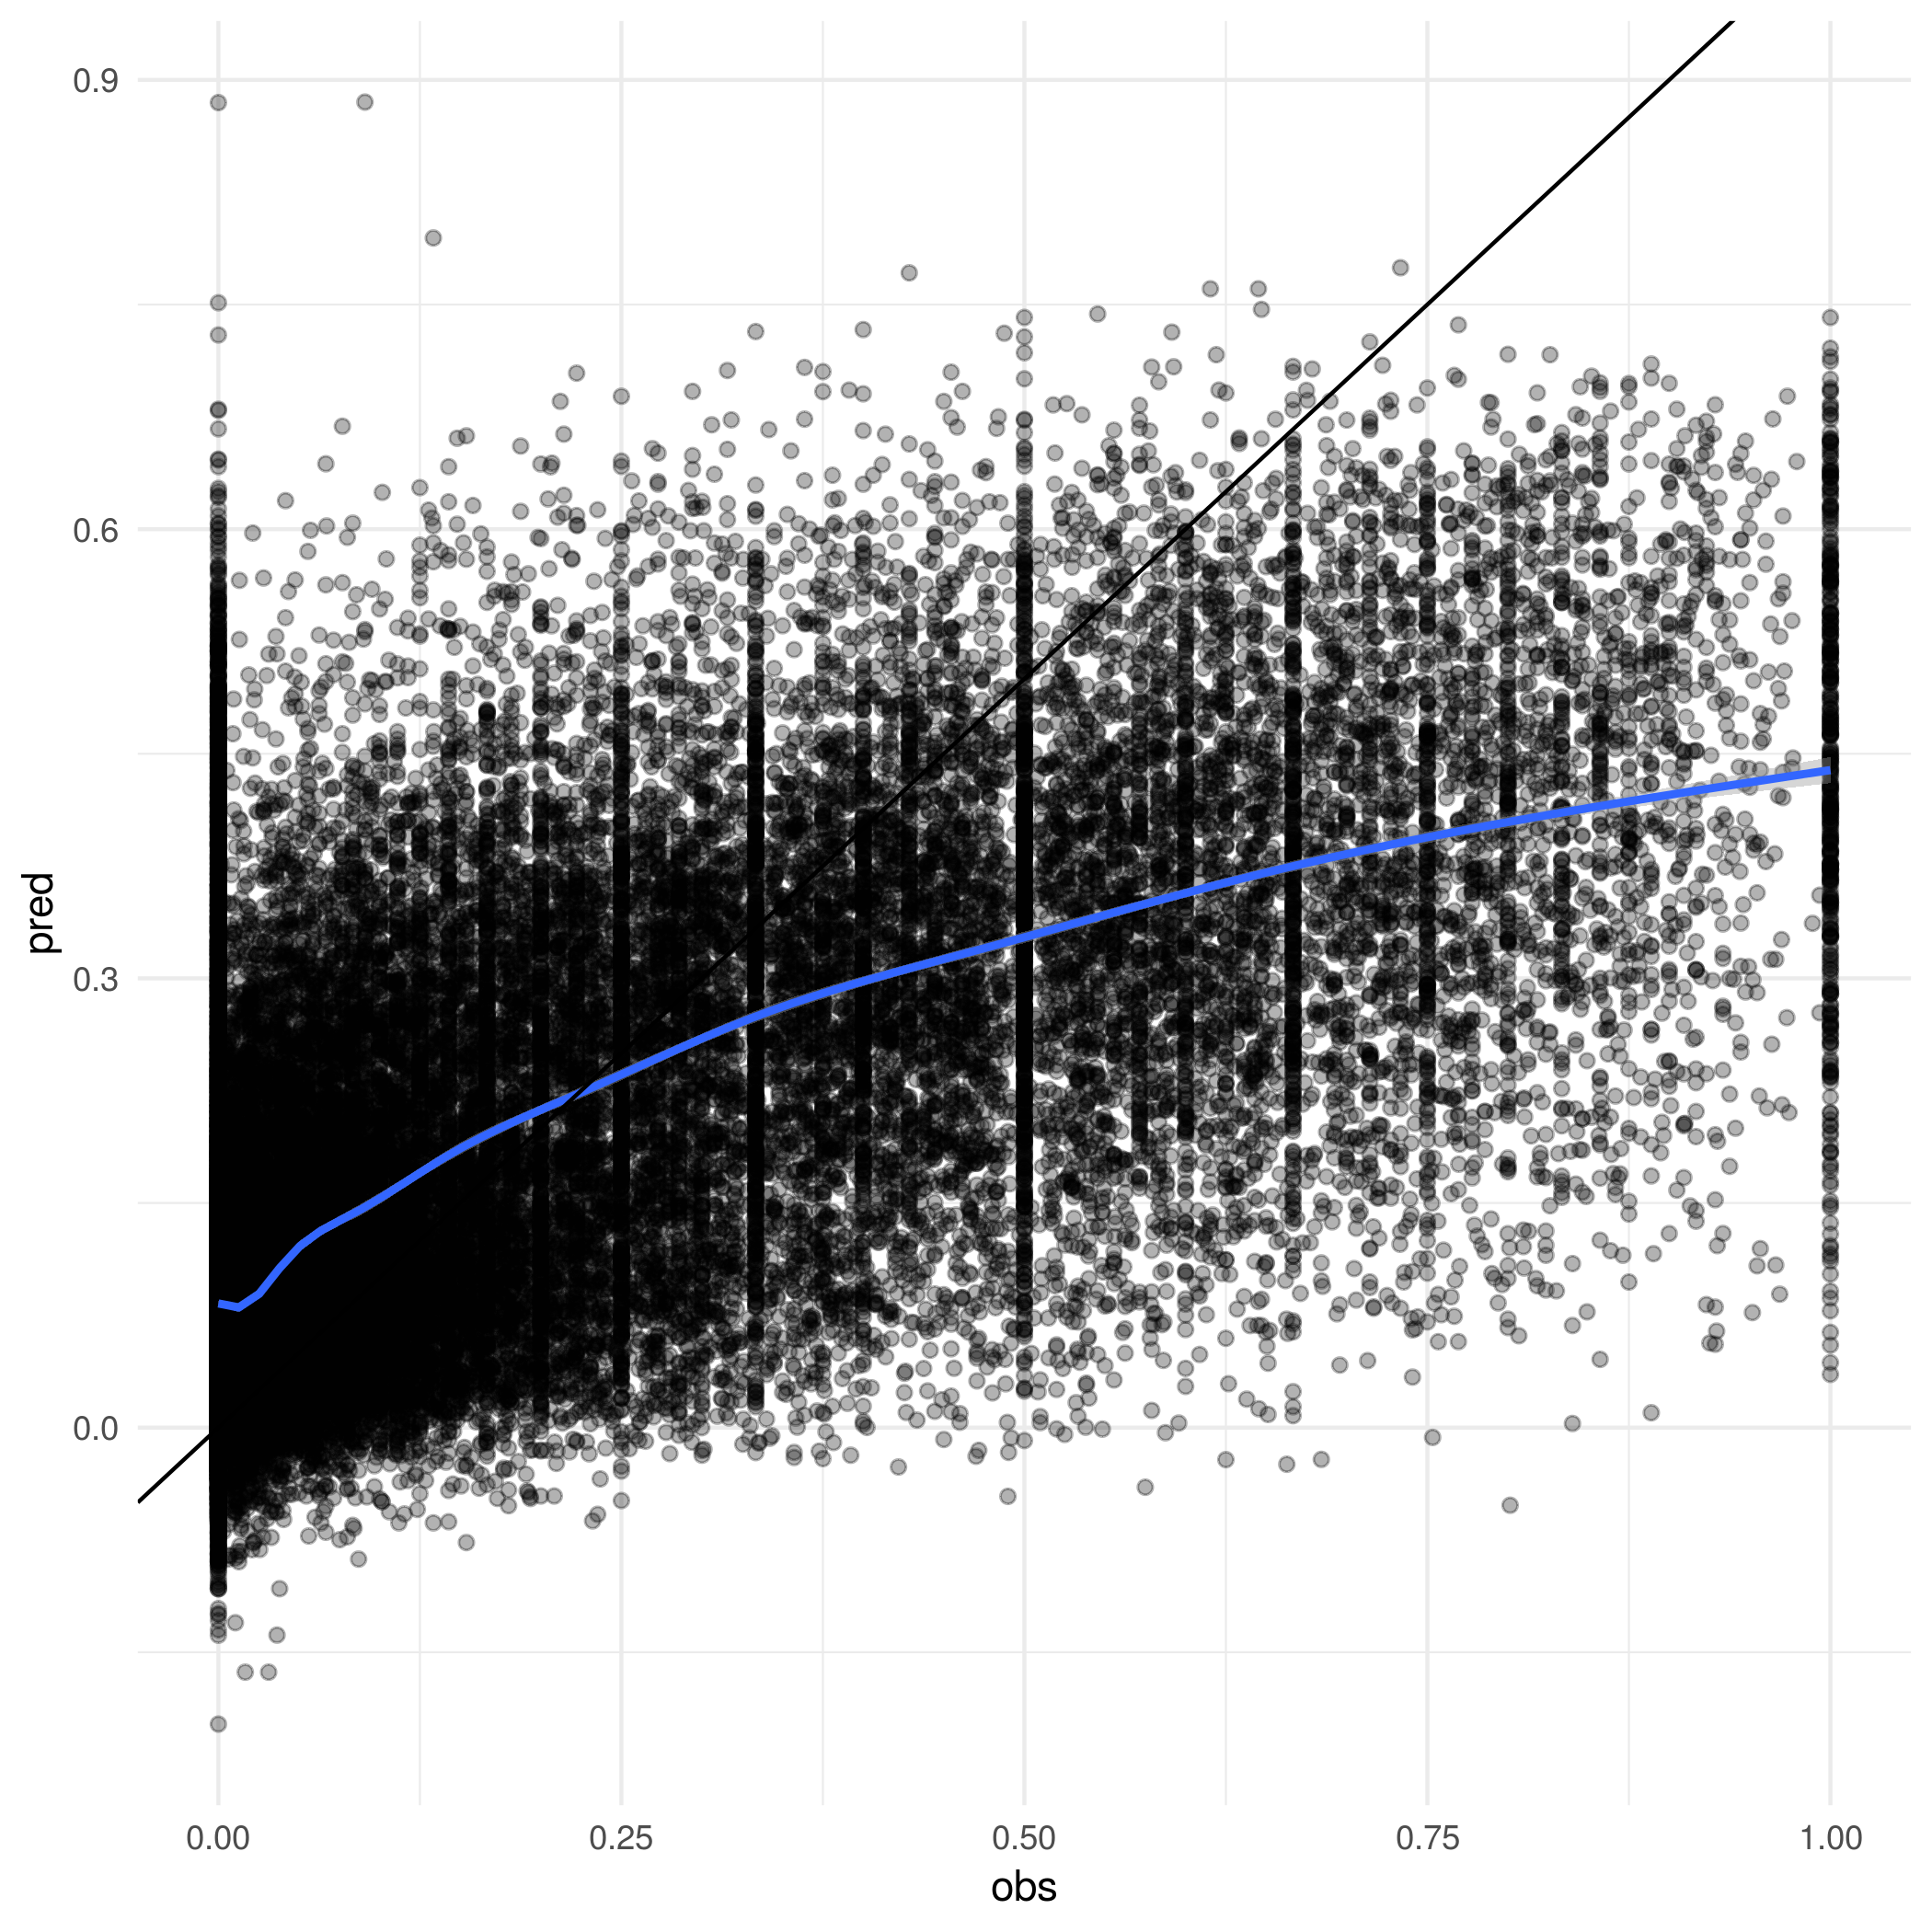
\includegraphics[width=0.6\textwidth]{figs/SI/gbm_obspred_global.png}
\caption{
  Scatter plot of predictions and held out observed data for the GBM trained on the global dataset.
}

\end{figure}


\clearpage
\subsection{Hyperparameter optimisation}

As ranger and GBM were tuned with random hyperparameter search, the plots become difficult and are not included.

\begin{figure}[h!]
  \centering
  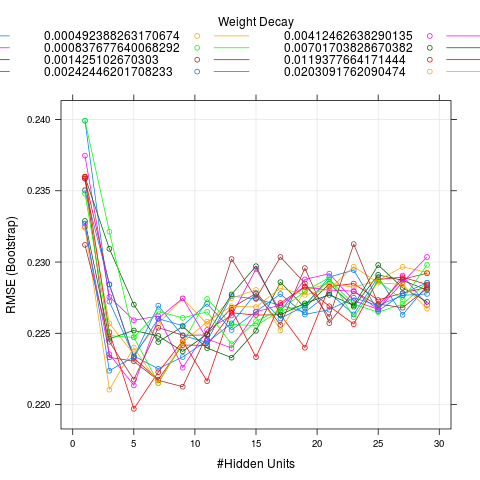
\includegraphics[width=0.6\textwidth]{figs/SI/nnetopt_global.png}
\caption{
  Optimisation for neural network hyperparameters trained on the global dataset.
}

\end{figure}


\begin{figure}[h!]
  \centering
  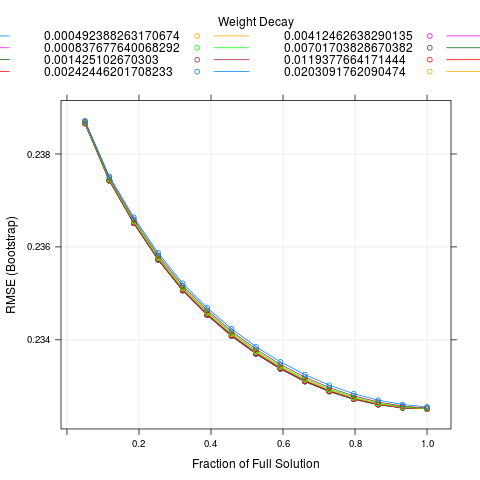
\includegraphics[width=0.6\textwidth]{figs/SI/enetopt_global.png}
\caption{
  Optimisation for elastic net hyperparameters trained on the global dataset.
}
\end{figure}



\begin{figure}[h!]
  \centering
  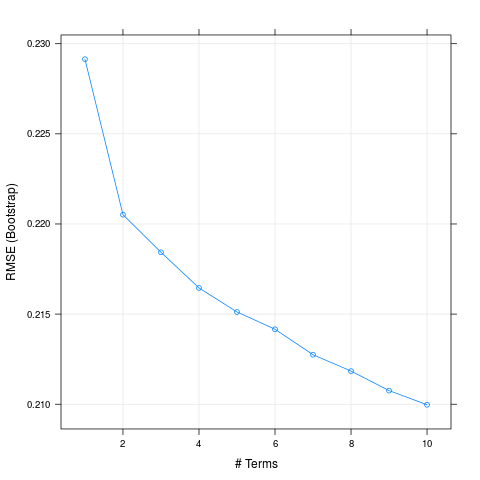
\includegraphics[width=0.6\textwidth]{figs/SI/ppropt.png}
\caption{
  Optimisation for PPR hyperparameters trained on the global dataset.
}

\end{figure}




\clearpage
%%%%%%%%%%%%%%%%%%%%%%%%%%%%%%%%%%%%%%%%%%%%%%%%%%%%%%%%%%%%%%%%%%%%%%%
\section{Colombia (South America) prevalence dataset Machine Learning}
%%%%%%%%%%%%%%%%%%%%%%%%%%%%%%%%%%%%%%%%%%%%%%%%%%%%%%%%%%%%%%%%%%%%%%%


\subsection{Predictions}

\begin{figure}[h!]
  \centering
  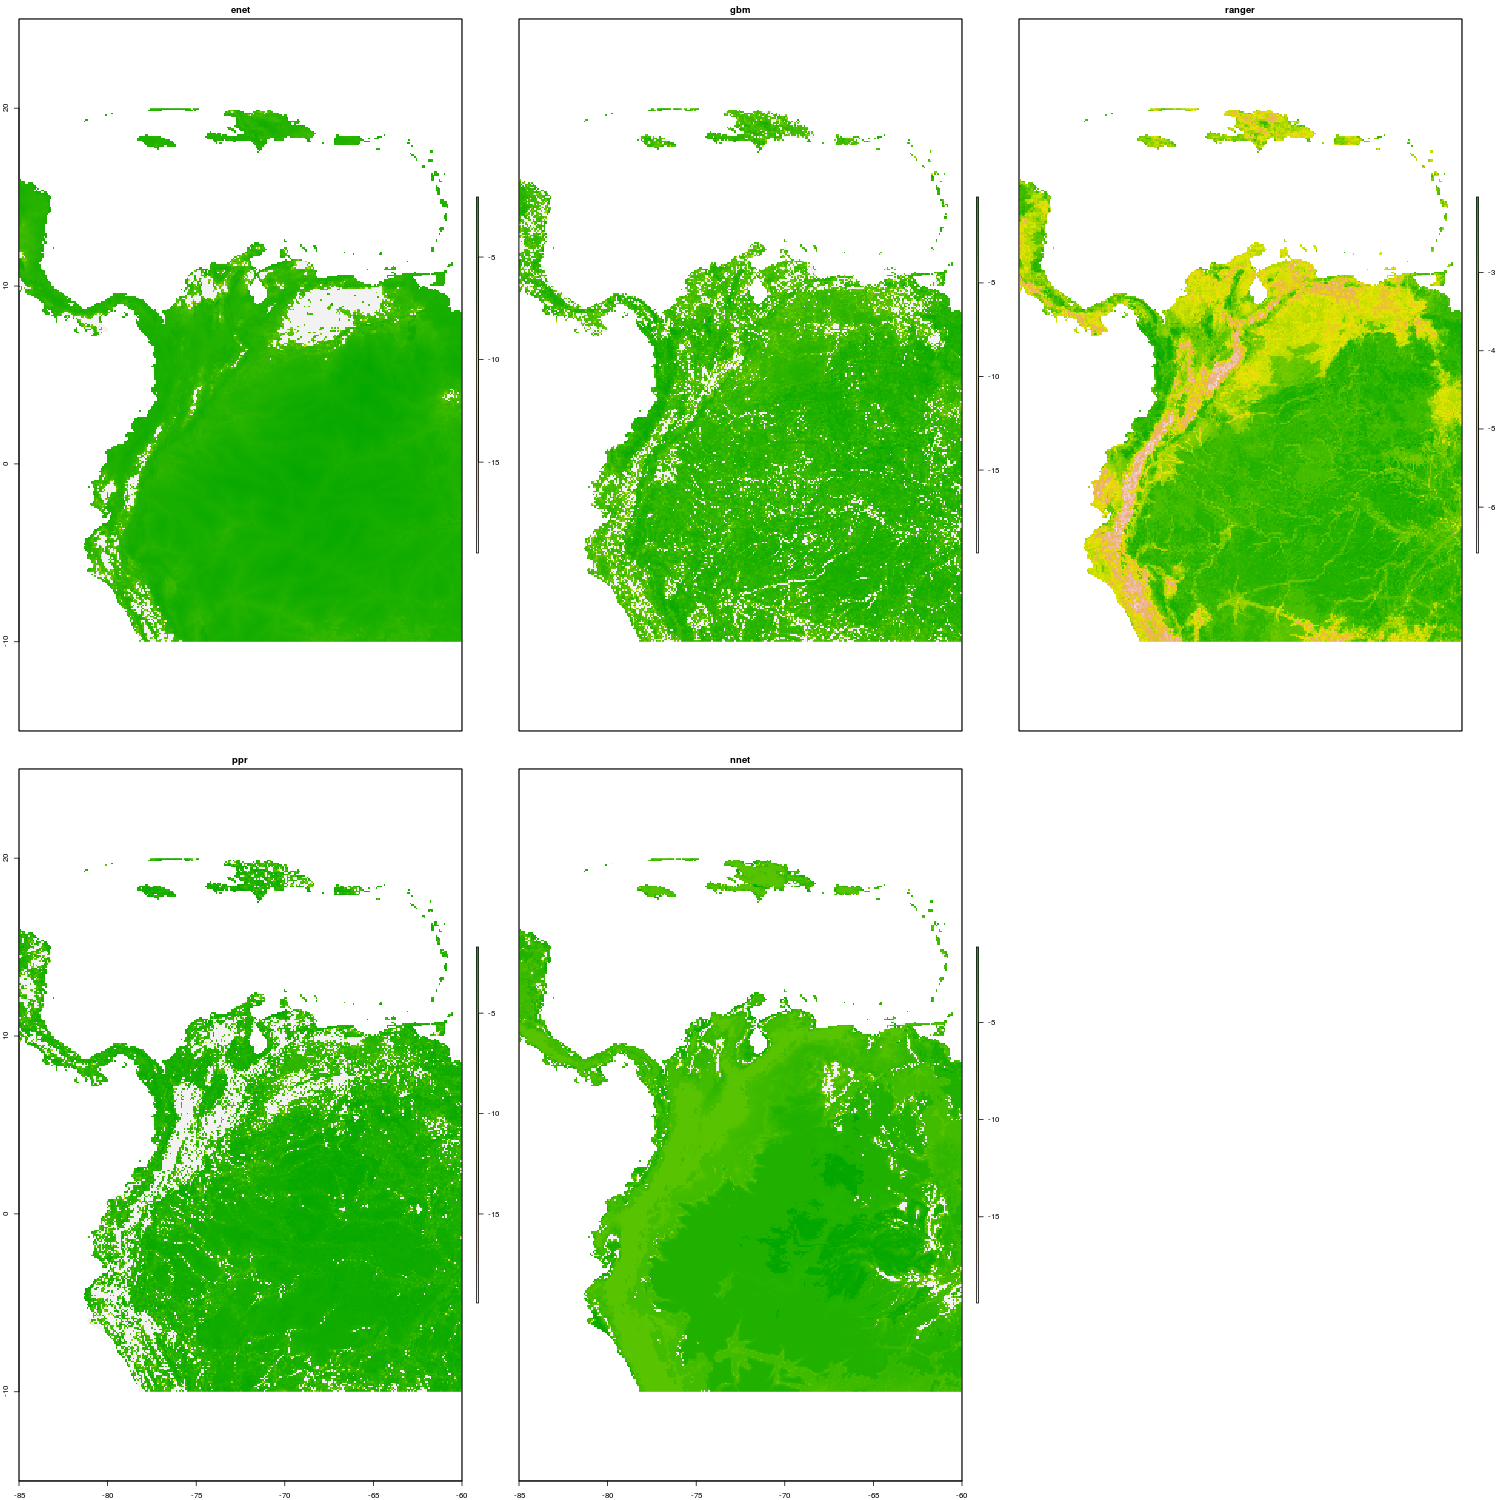
\includegraphics[width=1\textwidth]{figs/SI/SA_all_ml.png}
\caption{
  Predictions from machine learning models trained on South American prevalence data.
}

\end{figure}


\begin{figure}[h!]
  \centering
  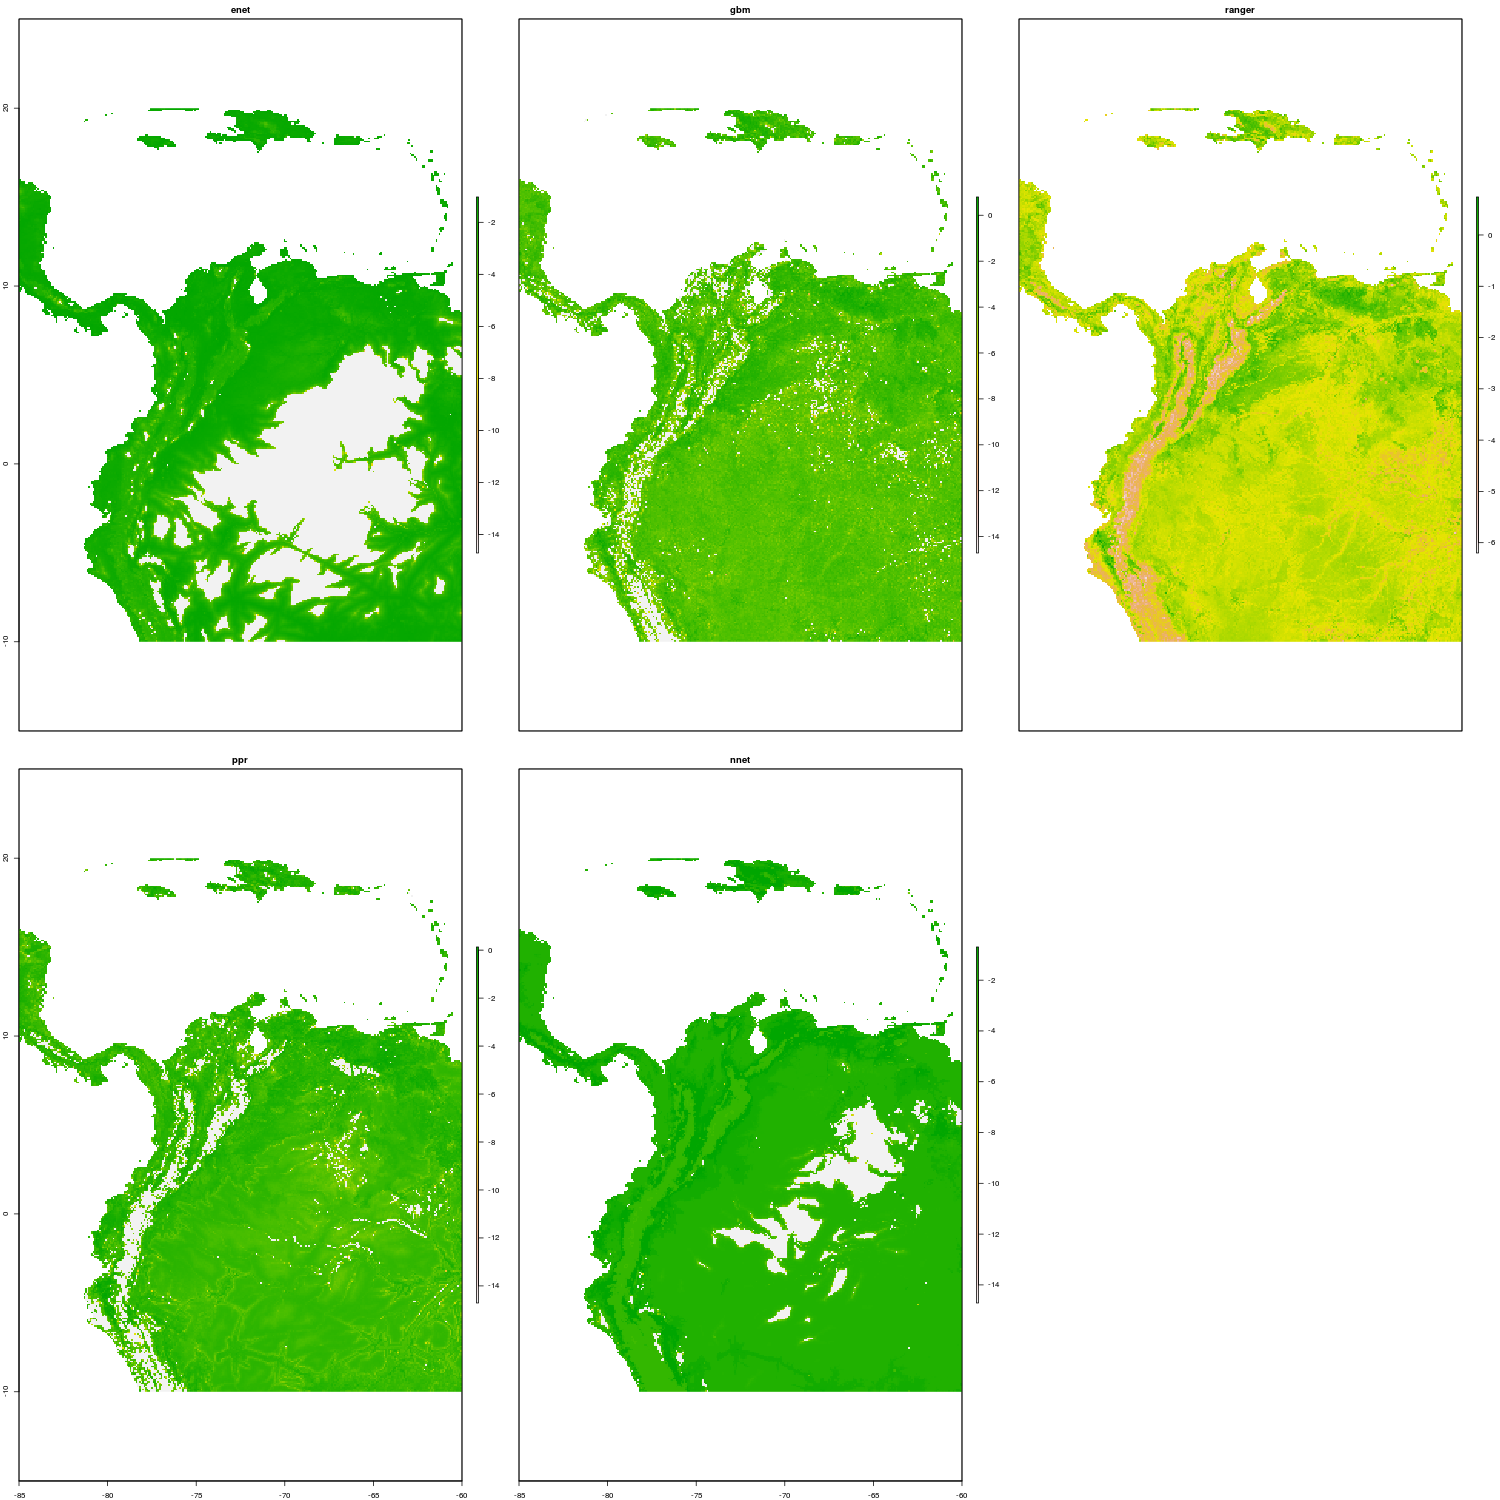
\includegraphics[width=1\textwidth]{figs/SI/COL_all_globalml.png}
\caption{
  Predictions over Colombia from machine learning models trained on global prevalence data.
}

\end{figure}




\clearpage
\subsection{Out-of-sample scatter plots}


\begin{figure}[h!]
  \centering
  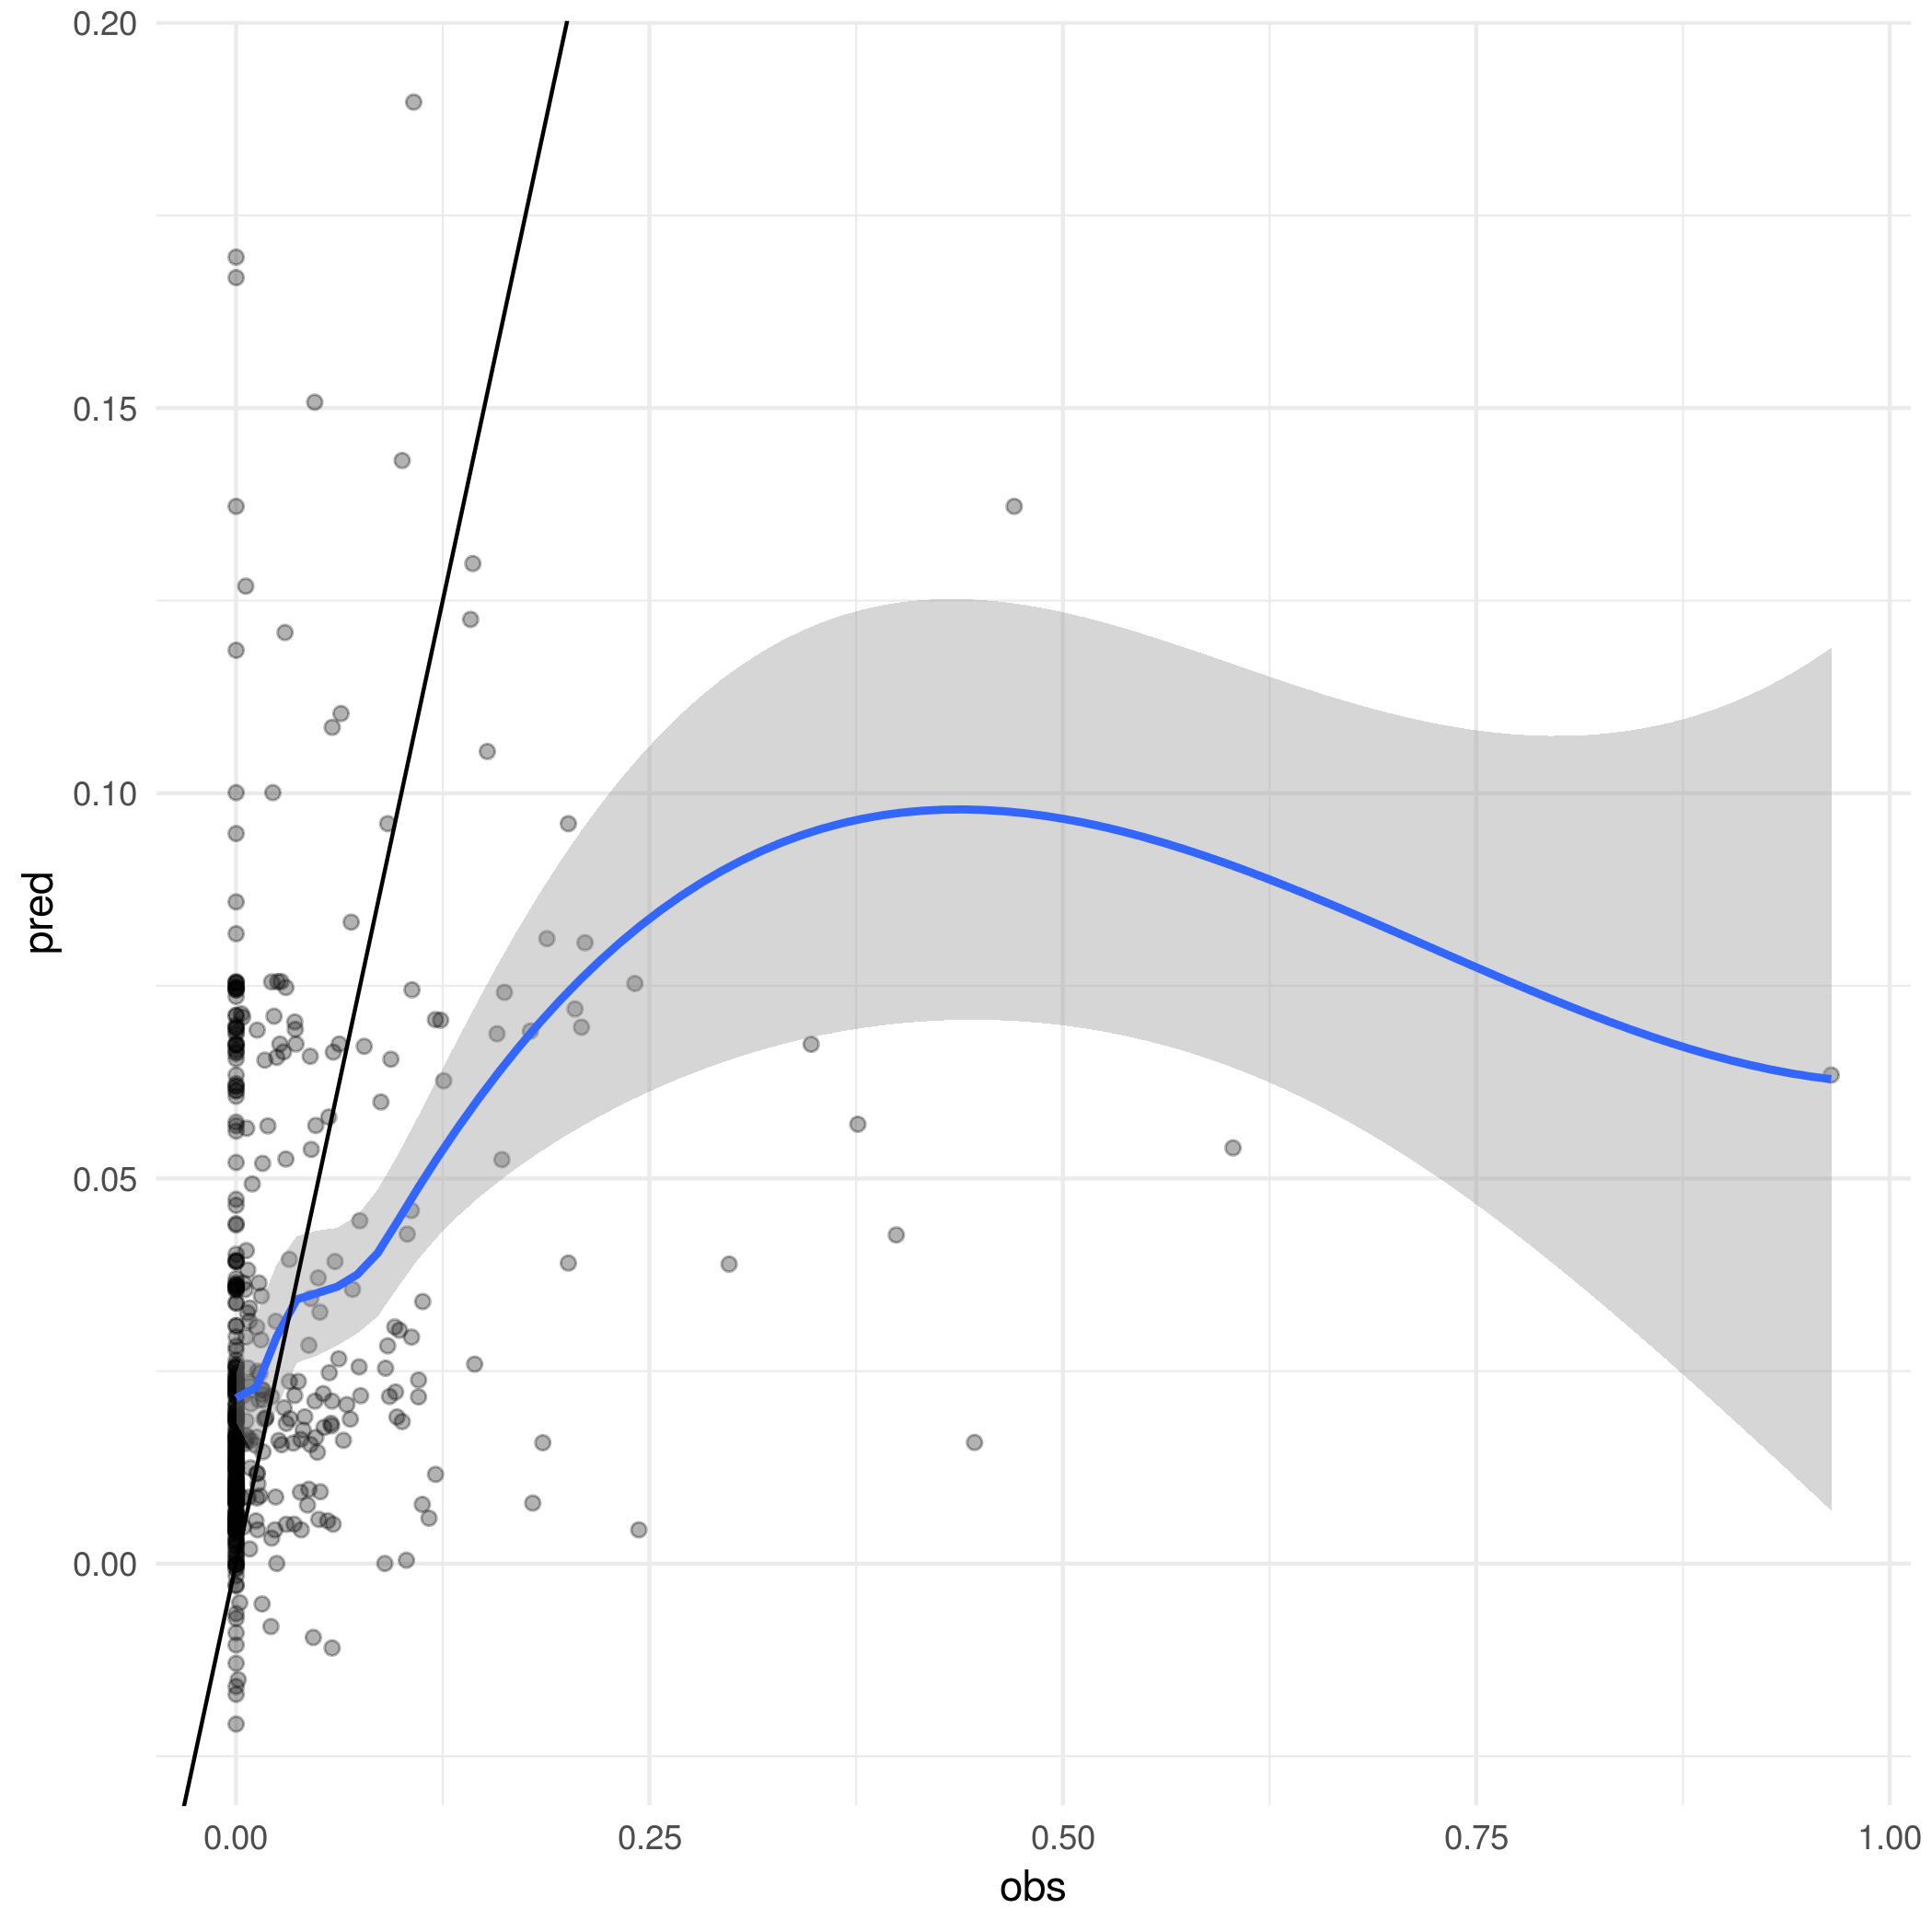
\includegraphics[width=0.6\textwidth]{figs/SI/nnet_obspred_sa.png}
\caption{
  Scatter plot of predictions and held out observed data for the neural network trained on the South America dataset.
}

\end{figure}



\begin{figure}[h!]
  \centering
  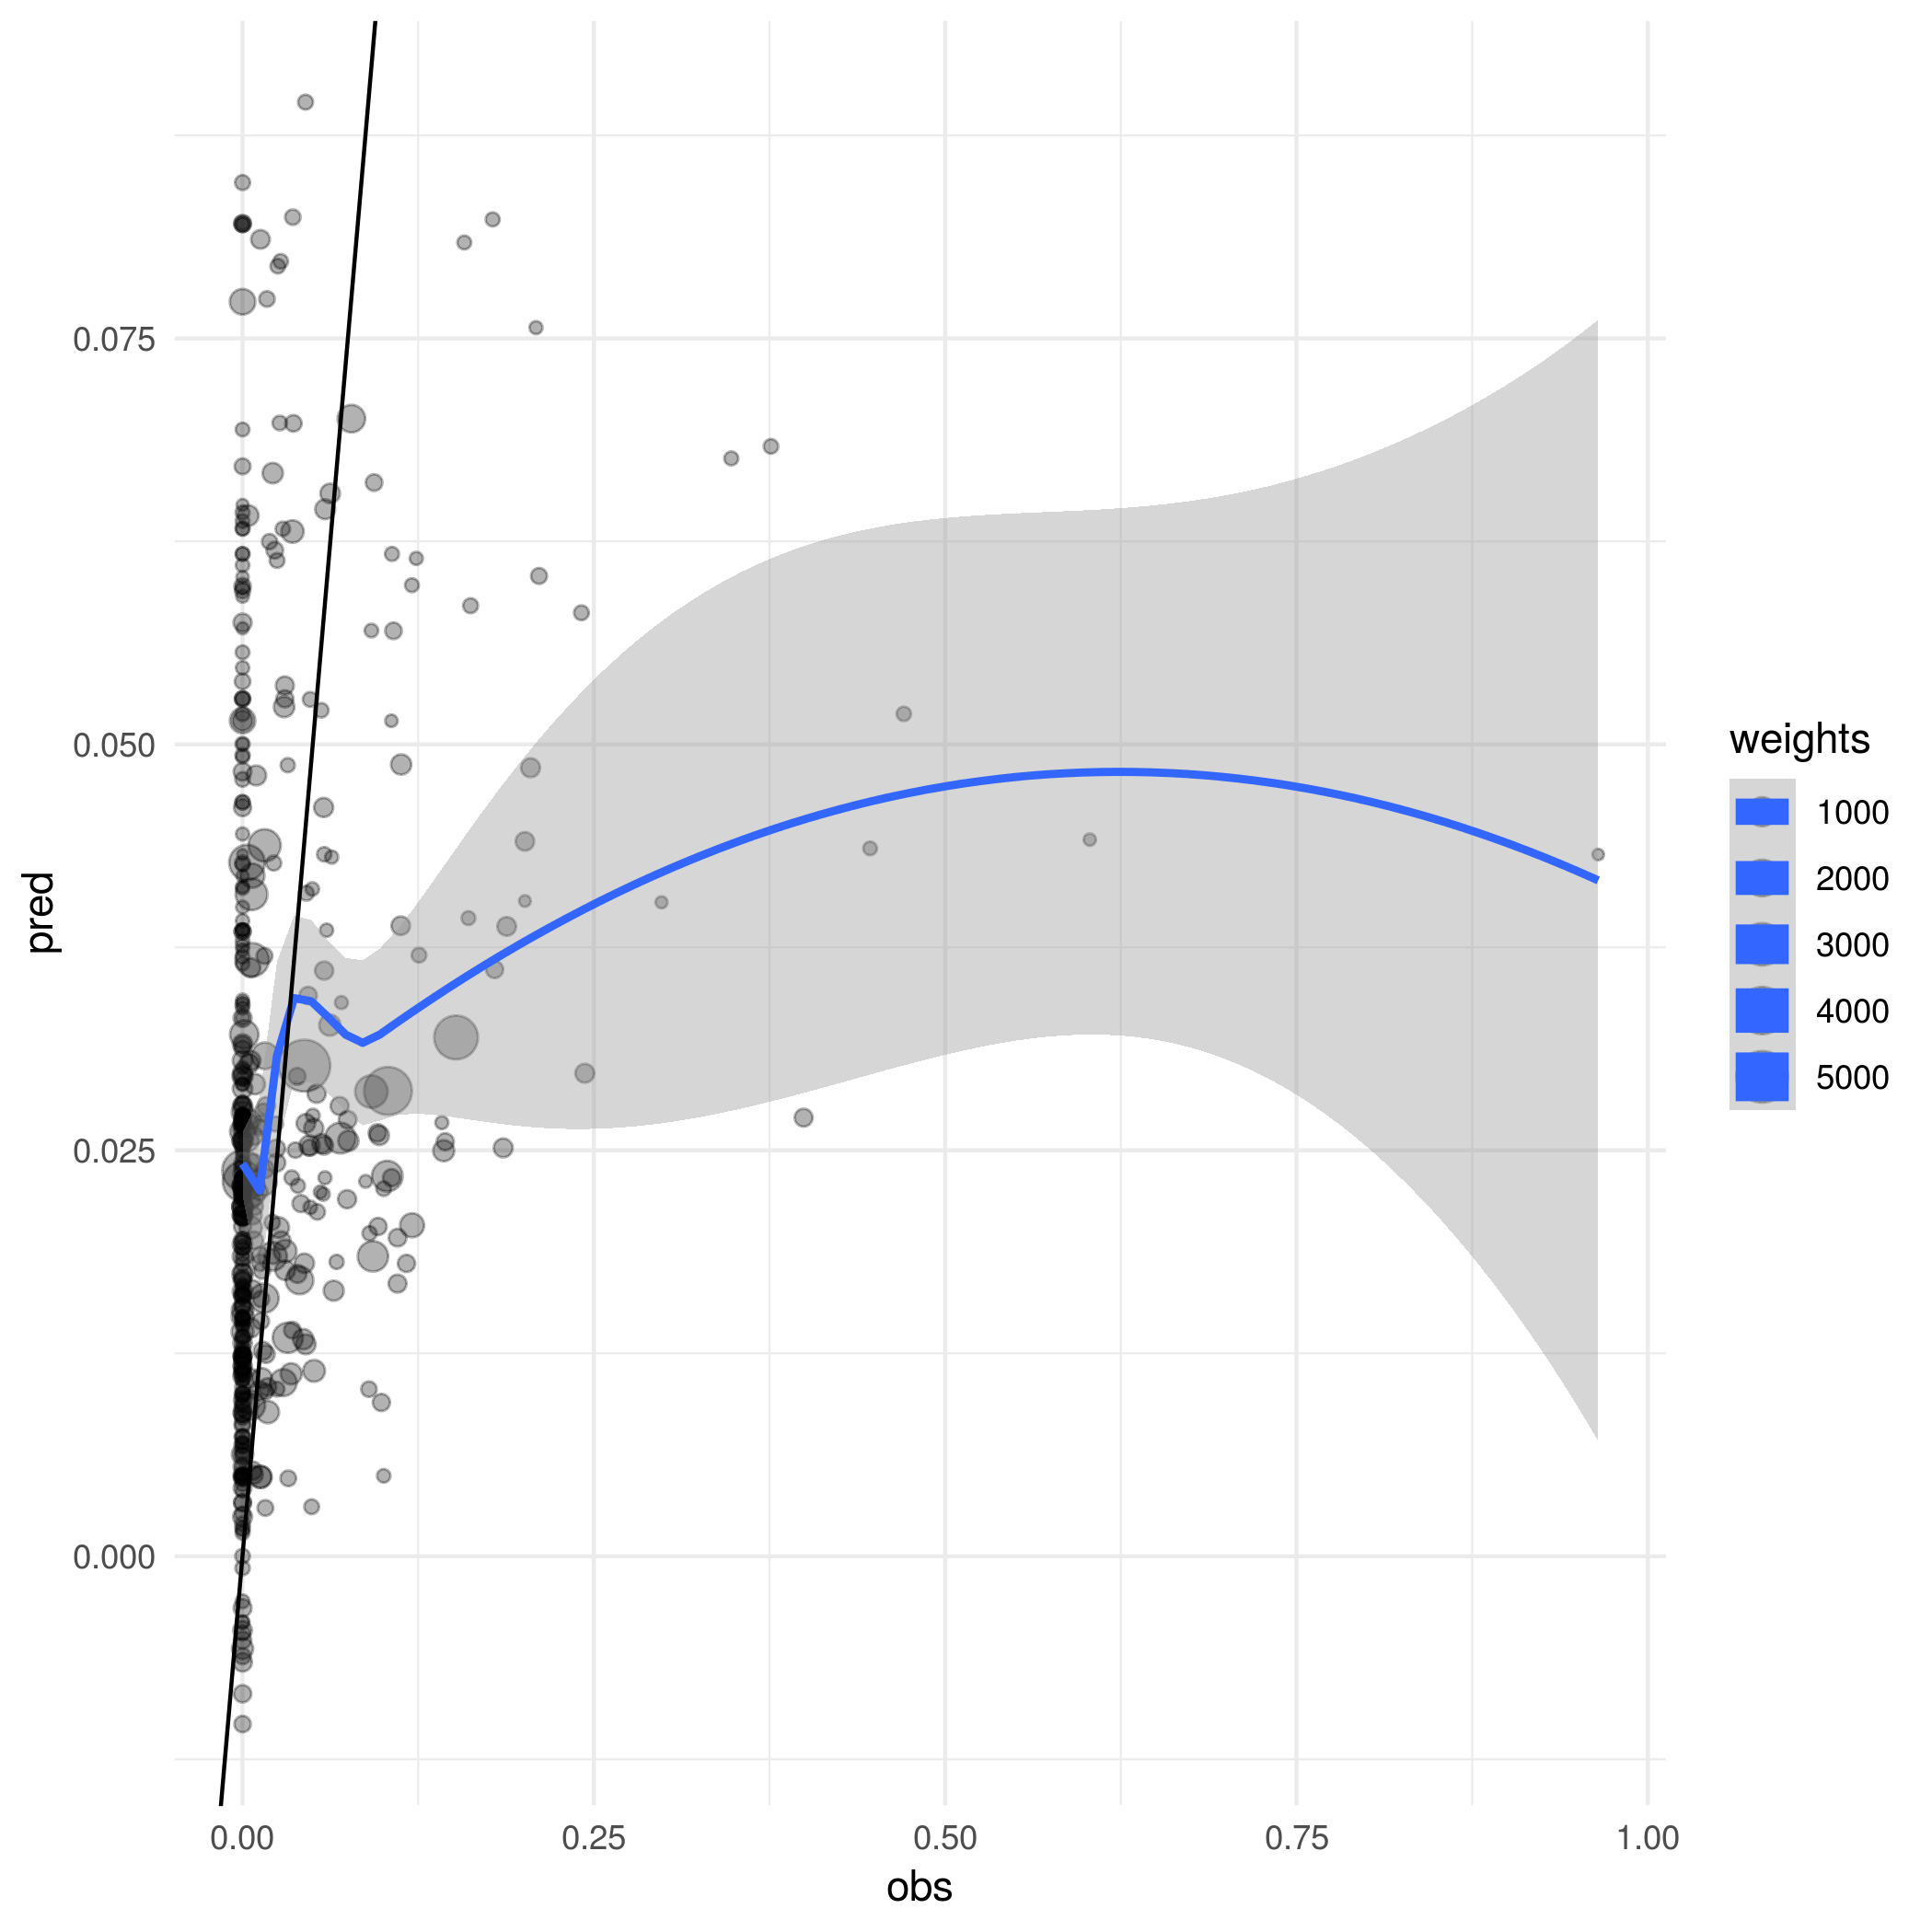
\includegraphics[width=0.6\textwidth]{figs/SI/enet_obspred_sa.png}
\caption{
  Scatter plot of predictions and held out observed data for the elastic net trained on the South America dataset.
}

\end{figure}


\begin{figure}[h!]
  \centering
  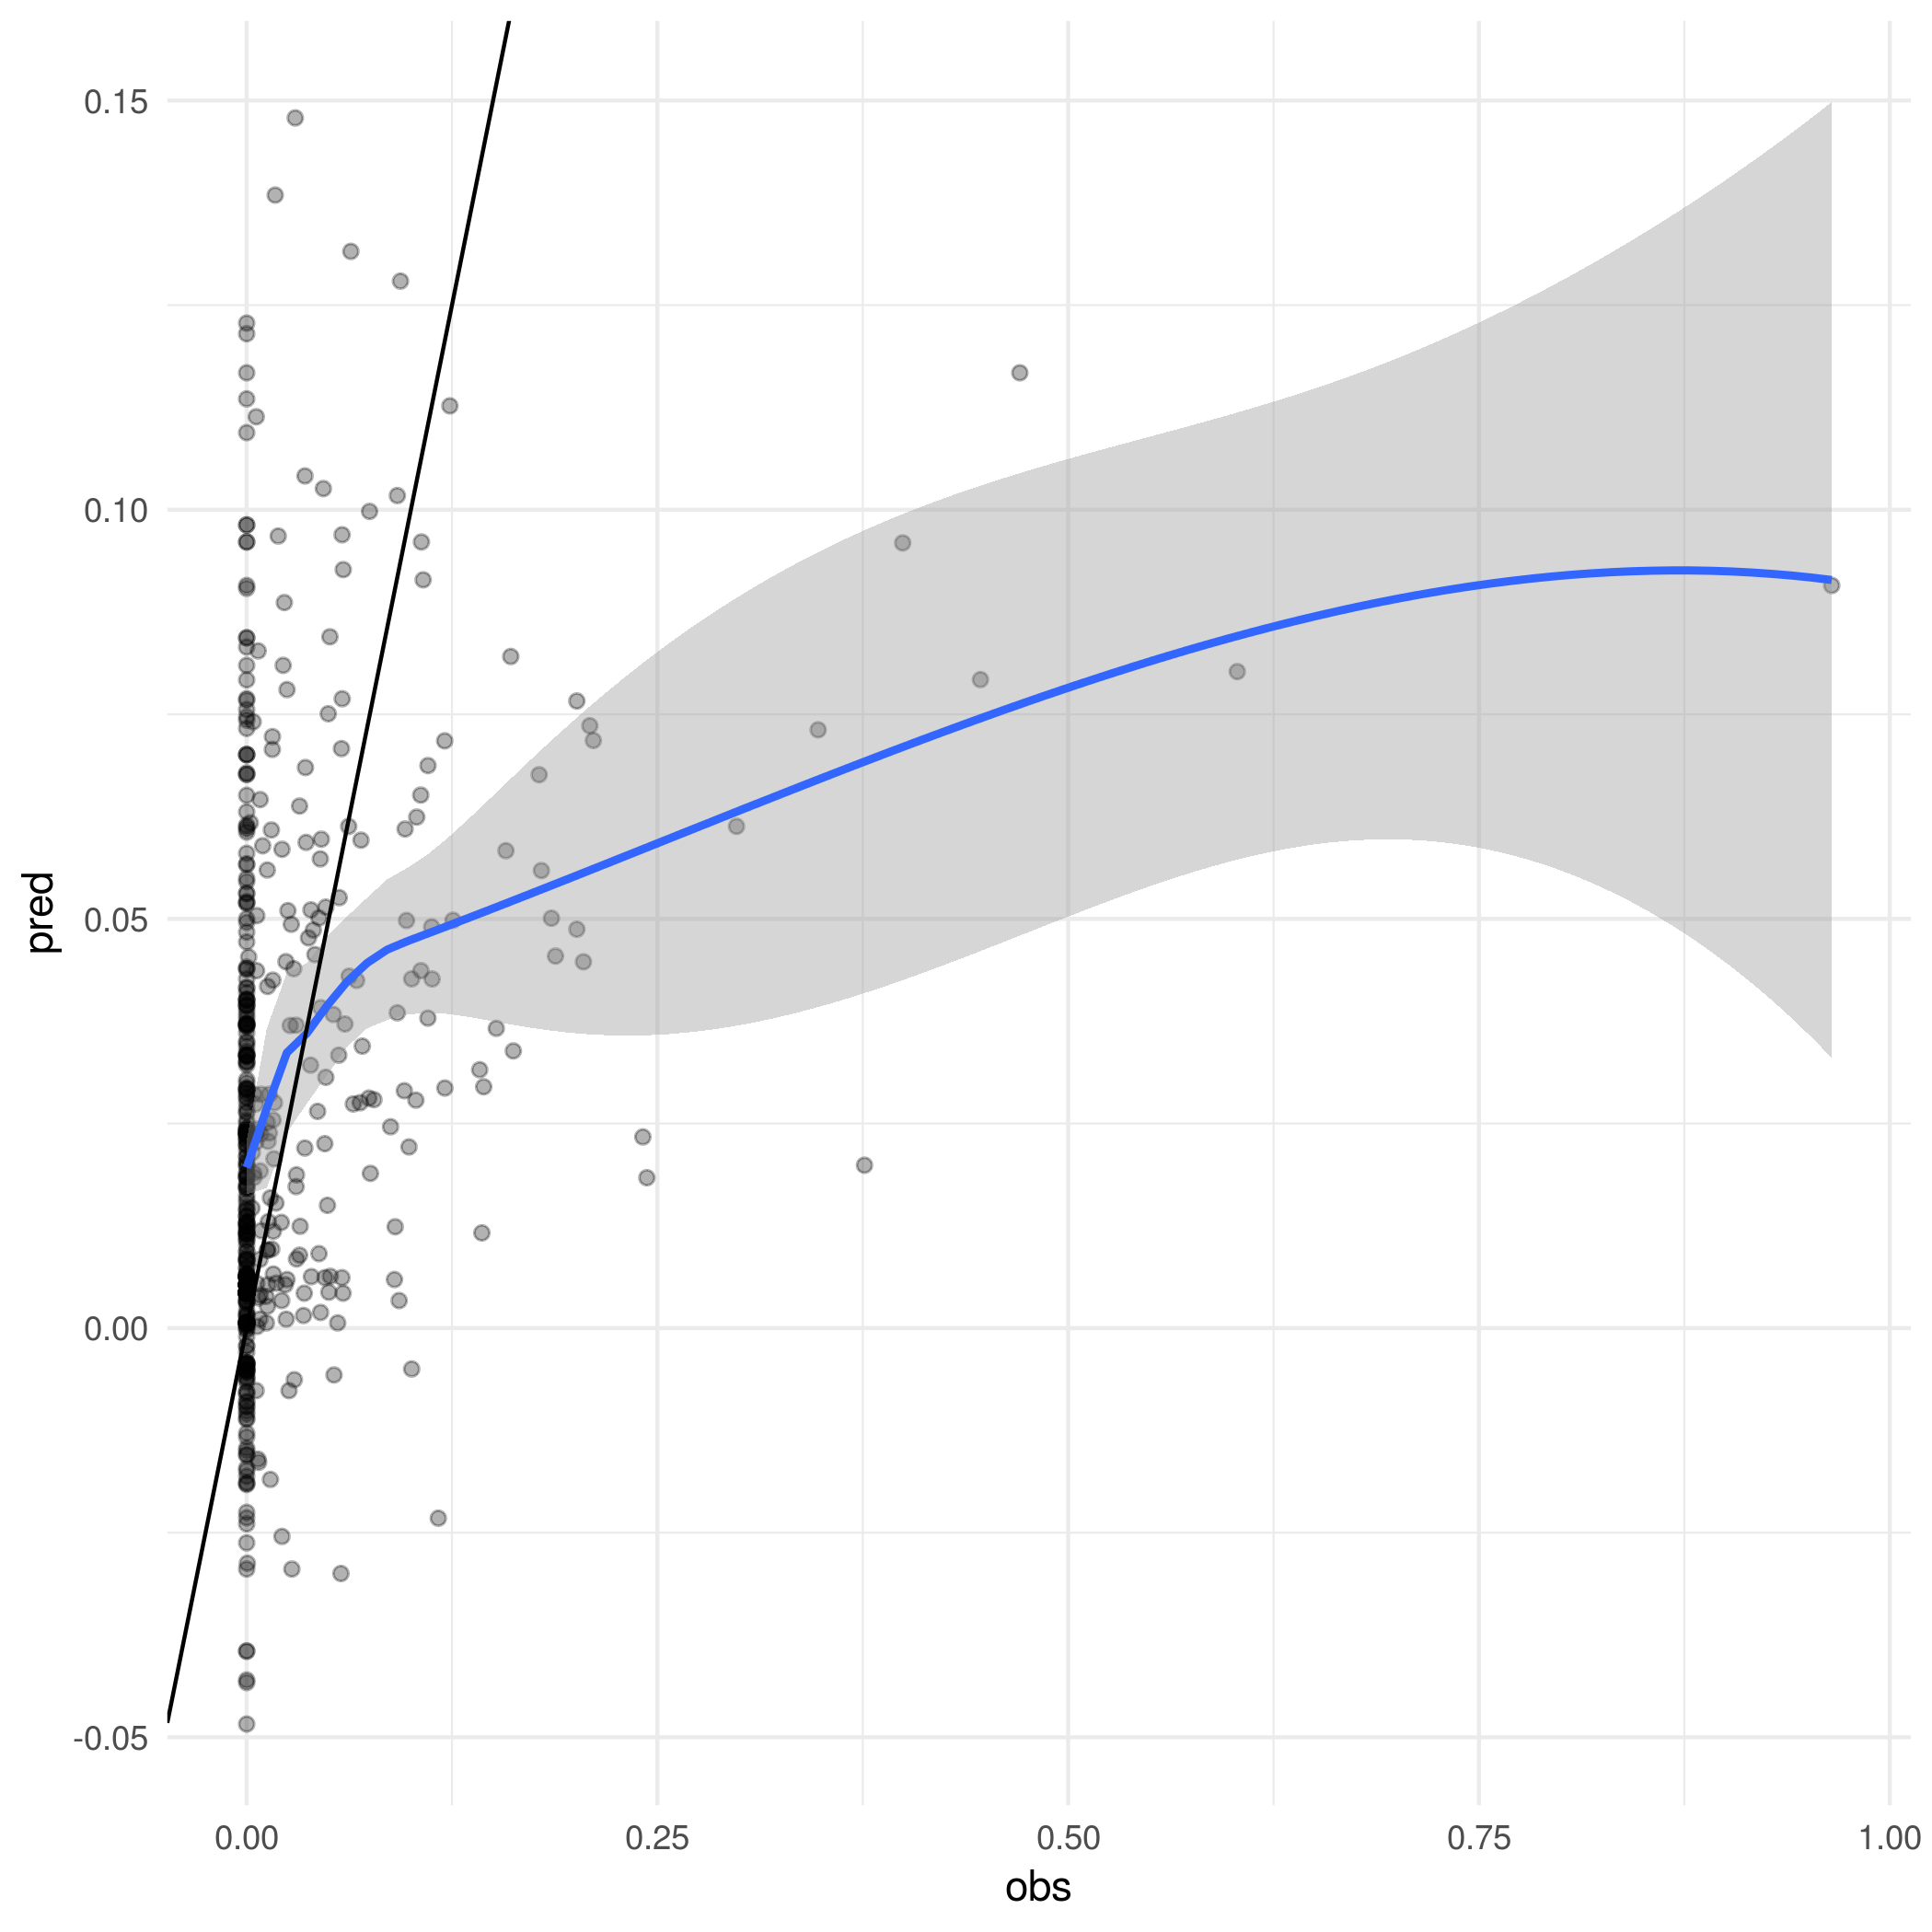
\includegraphics[width=0.6\textwidth]{figs/SI/ppr_obspred_sa.png}
\caption{
  Scatter plot of predictions and held out observed data for the PPR trained on the South America dataset.
}

\end{figure}


\begin{figure}[h!]
  \centering
  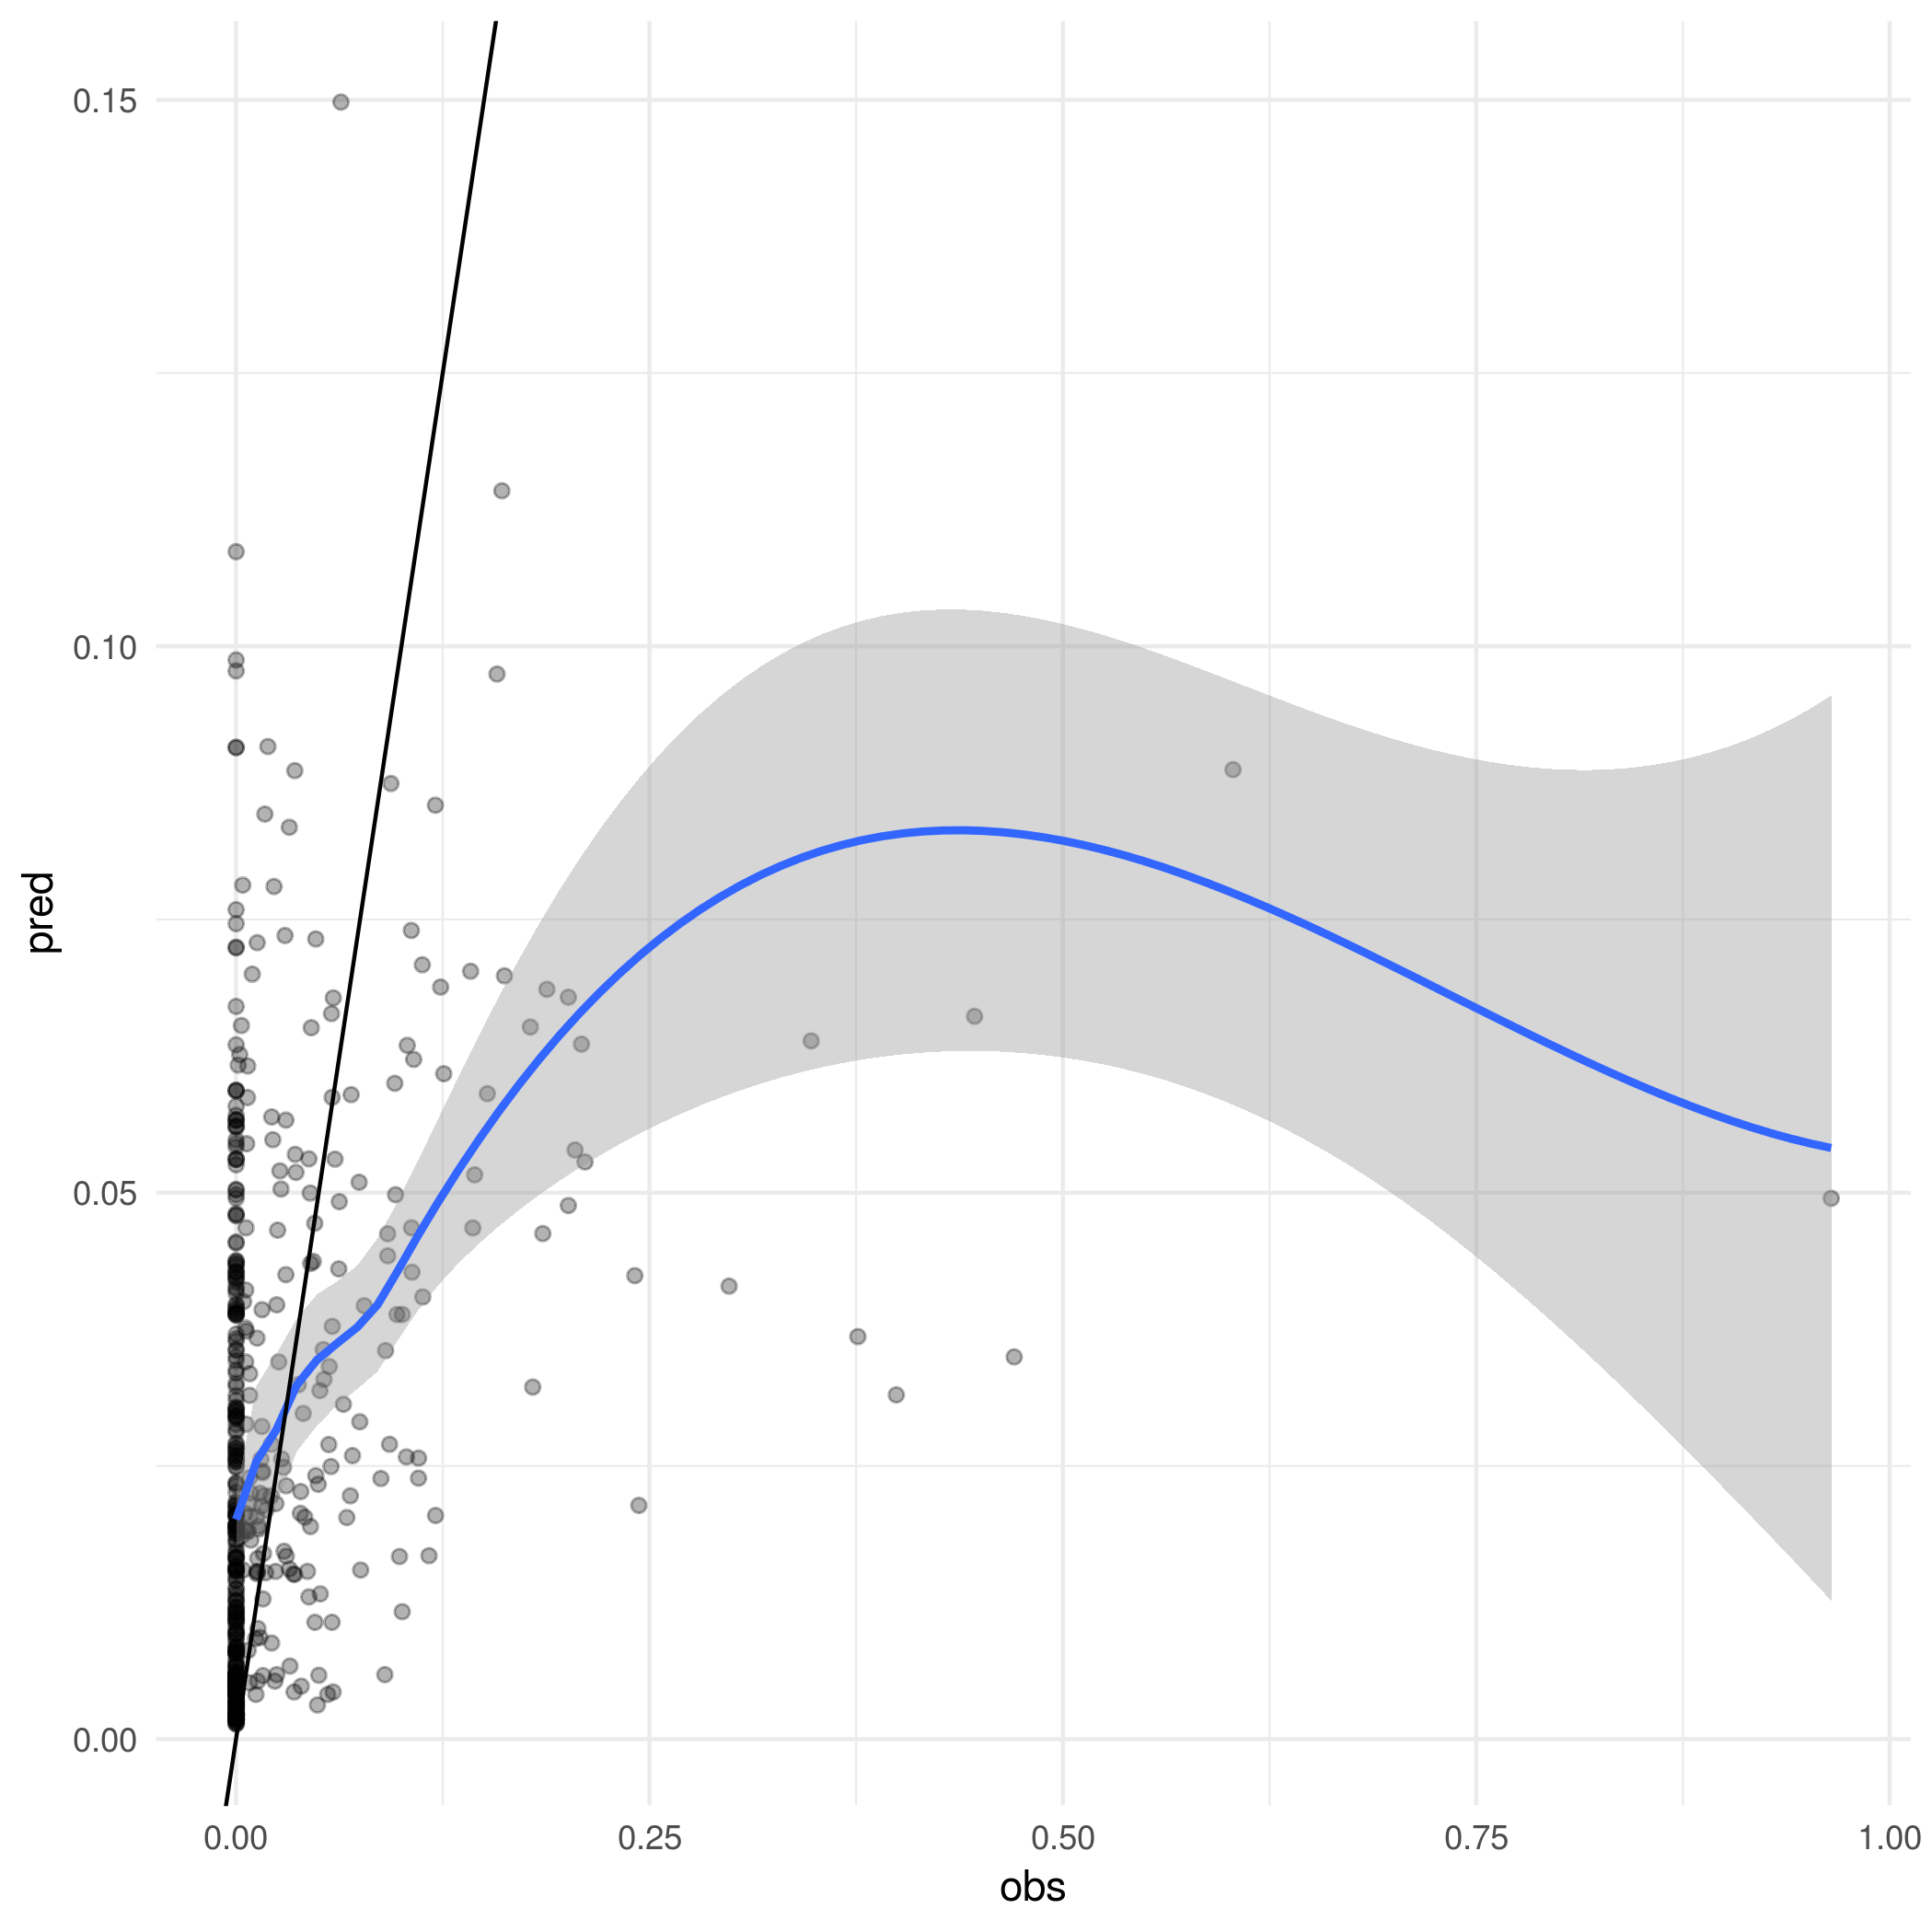
\includegraphics[width=0.6\textwidth]{figs/SI/ranger_obspred_sa.png}
\caption{
  Scatter plot of predictions and held out observed data for the Random Forest trained on the South America dataset.
}

\end{figure}


\begin{figure}[h!]
  \centering
  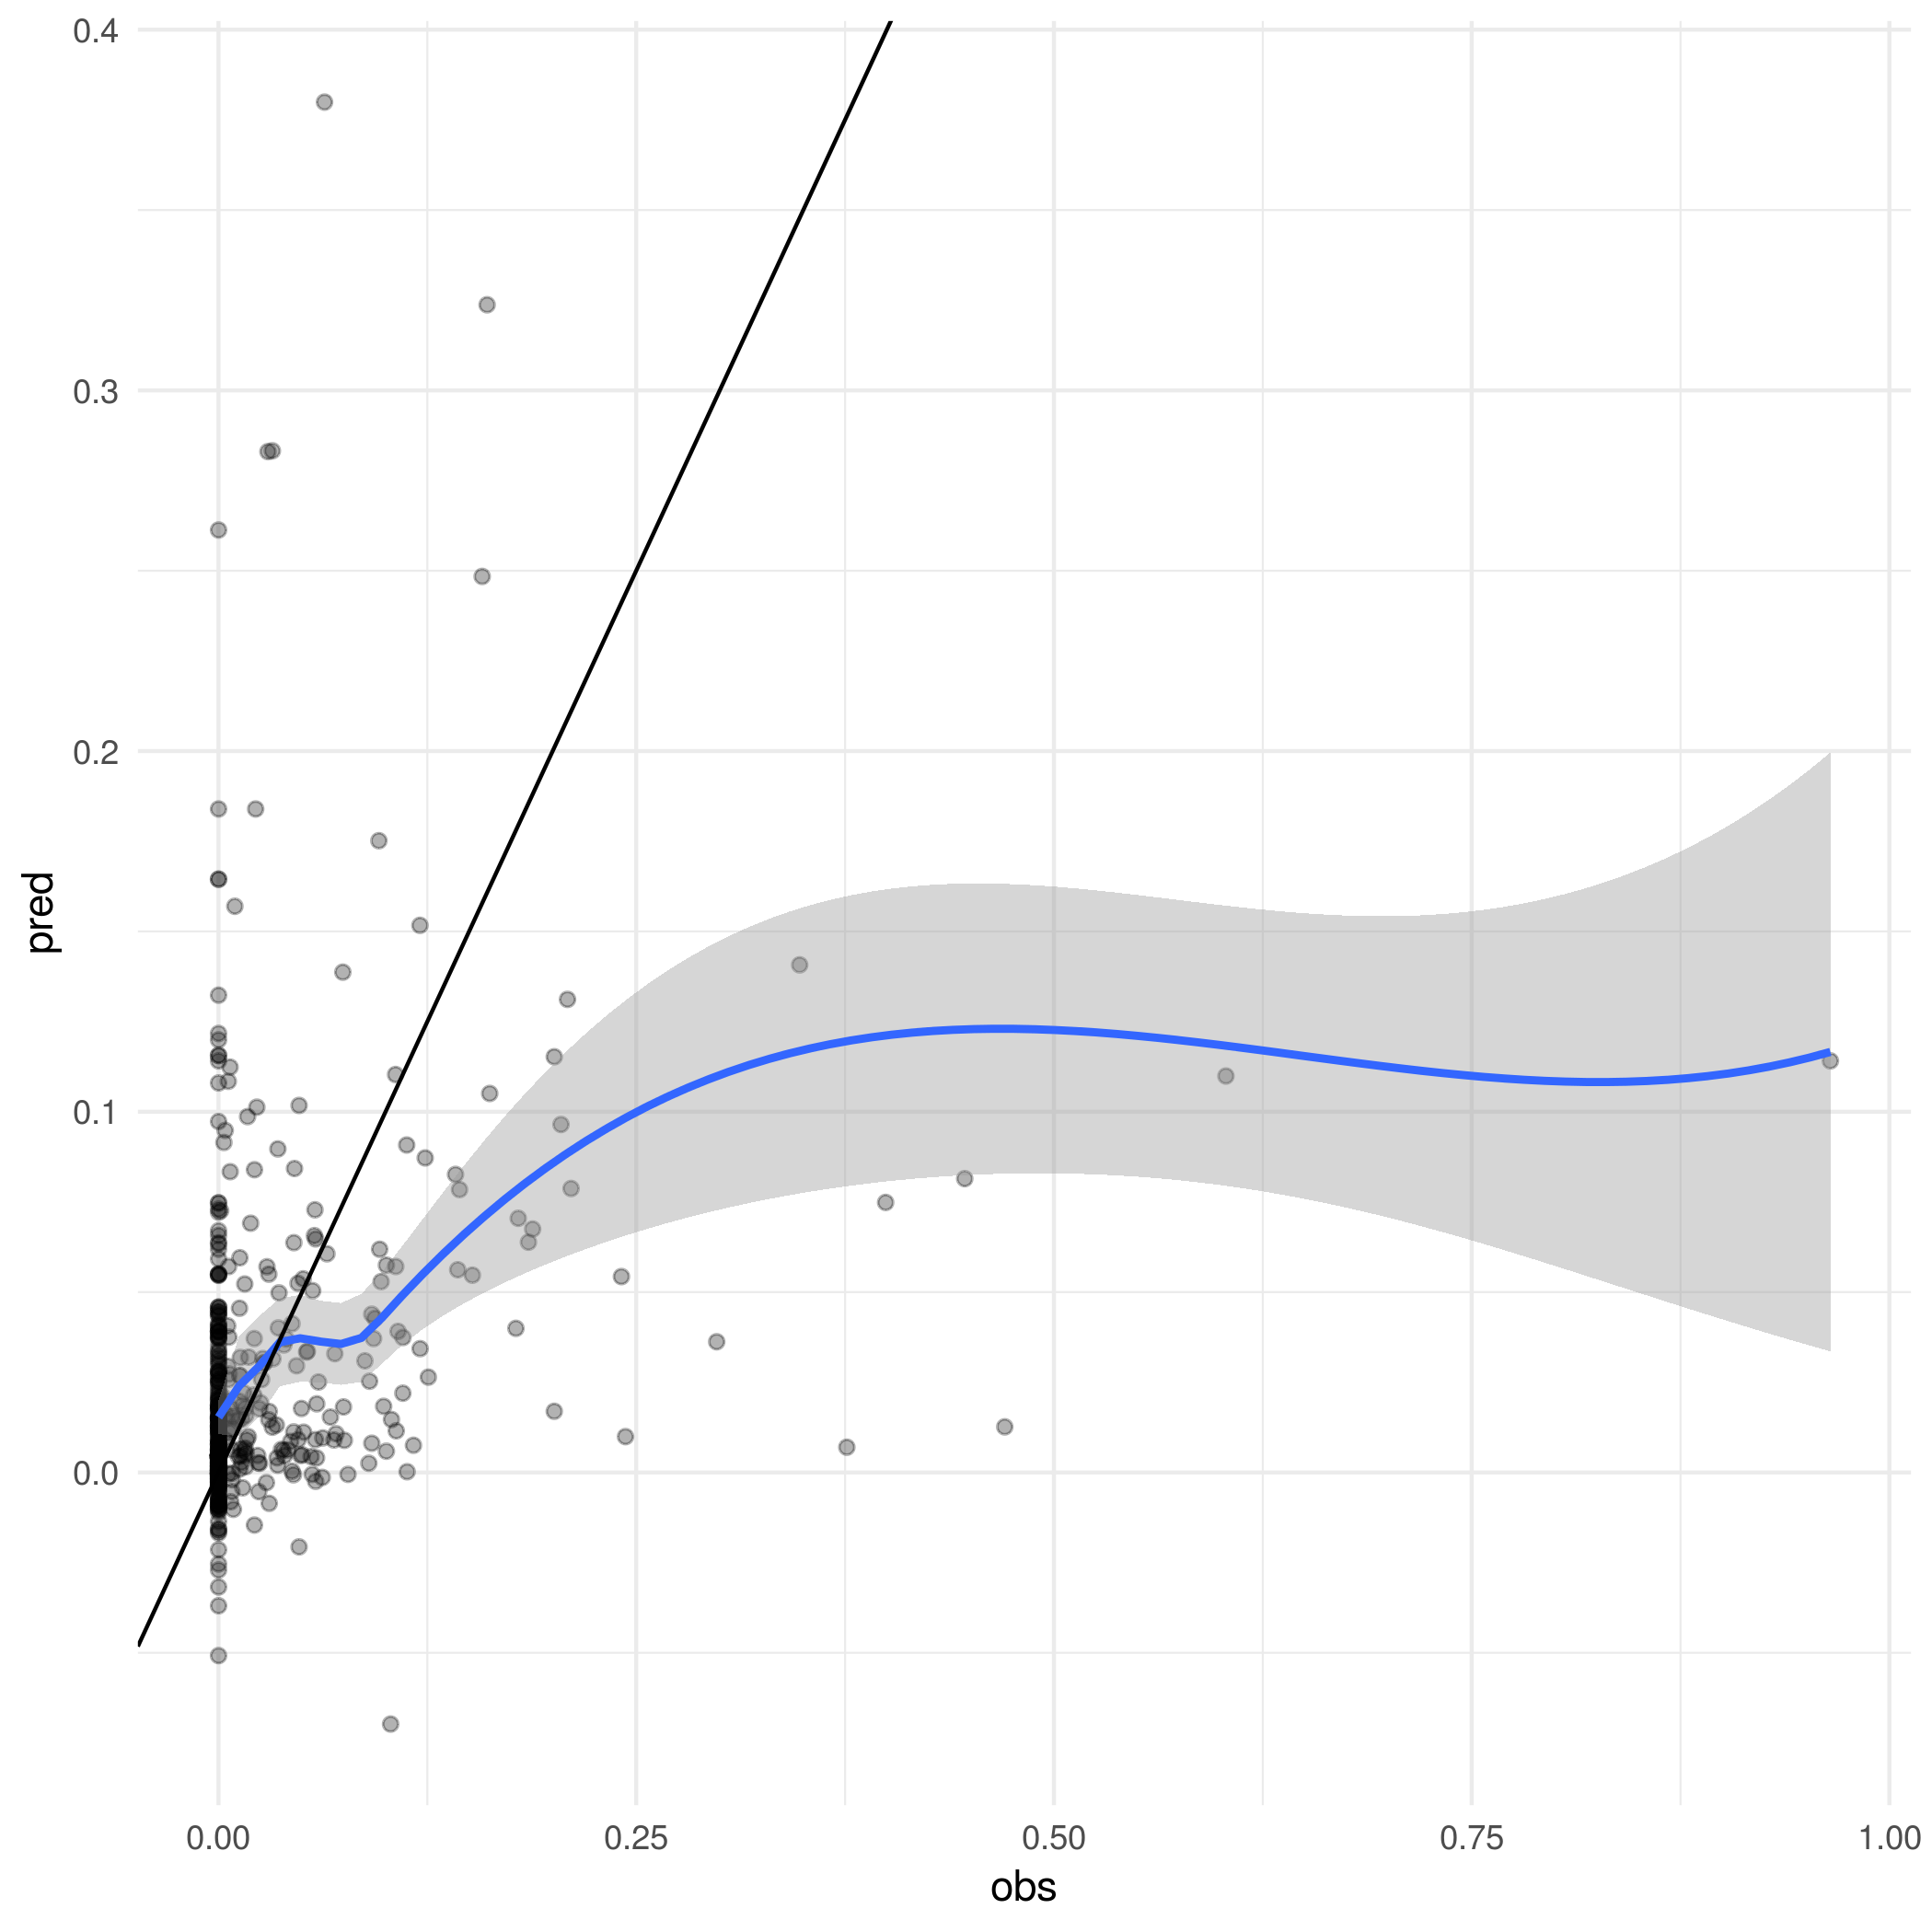
\includegraphics[width=0.6\textwidth]{figs/SI/gbm_obspred_sa.png}
\caption{
  Scatter plot of predictions and held out observed data for the GBM trained on the South America dataset.
}

\end{figure}


\clearpage
\subsection{Hyperparameter optimisation}

As ranger and GBM were tuned with random hyperparameter search, the plots become difficult and are not included.

\begin{figure}[h!]
  \centering
  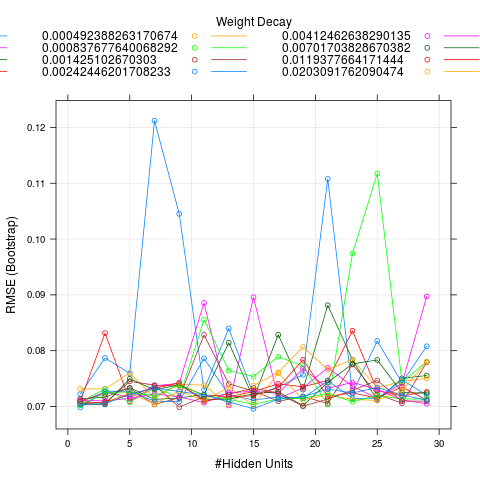
\includegraphics[width=0.6\textwidth]{figs/SI/nnetopt_sa.png}
\caption{
  Optimisation for neural network hyperparameters trained on the South America dataset.
}

\end{figure}


\begin{figure}[h!]
  \centering
  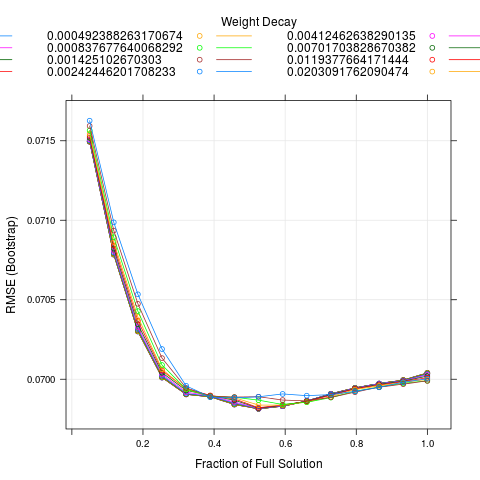
\includegraphics[width=0.6\textwidth]{figs/SI/enetopt_sa.png}
\caption{
  Optimisation for elastic net hyperparameters trained on the South America dataset.
}
\end{figure}



\begin{figure}[h!]
  \centering
  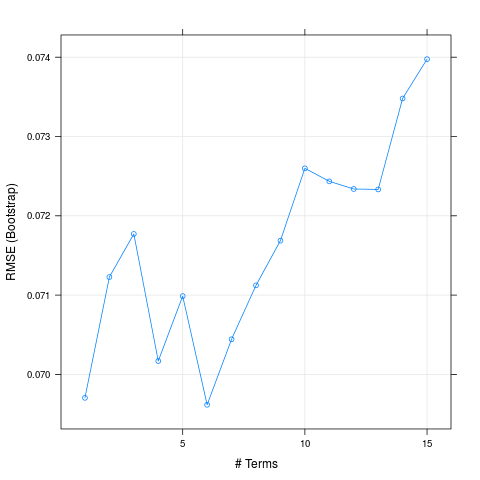
\includegraphics[width=0.6\textwidth]{figs/SI/ppropt_sa.png}
\caption{
  Optimisation for PPR hyperparameters trained on the South America dataset.
}

\end{figure}












\clearpage
%%%%%%%%%%%%%%%%%%%%%%%%%%%%%%%%%%%%%%%%%%%%%%%%%%%%%%%%%%%%%%%%%%%%%%%
\section{Indonesia dataset Machine Learning}
%%%%%%%%%%%%%%%%%%%%%%%%%%%%%%%%%%%%%%%%%%%%%%%%%%%%%%%%%%%%%%%%%%%%%%%



\subsection{Predictions}

\begin{figure}[h!]
  \centering
  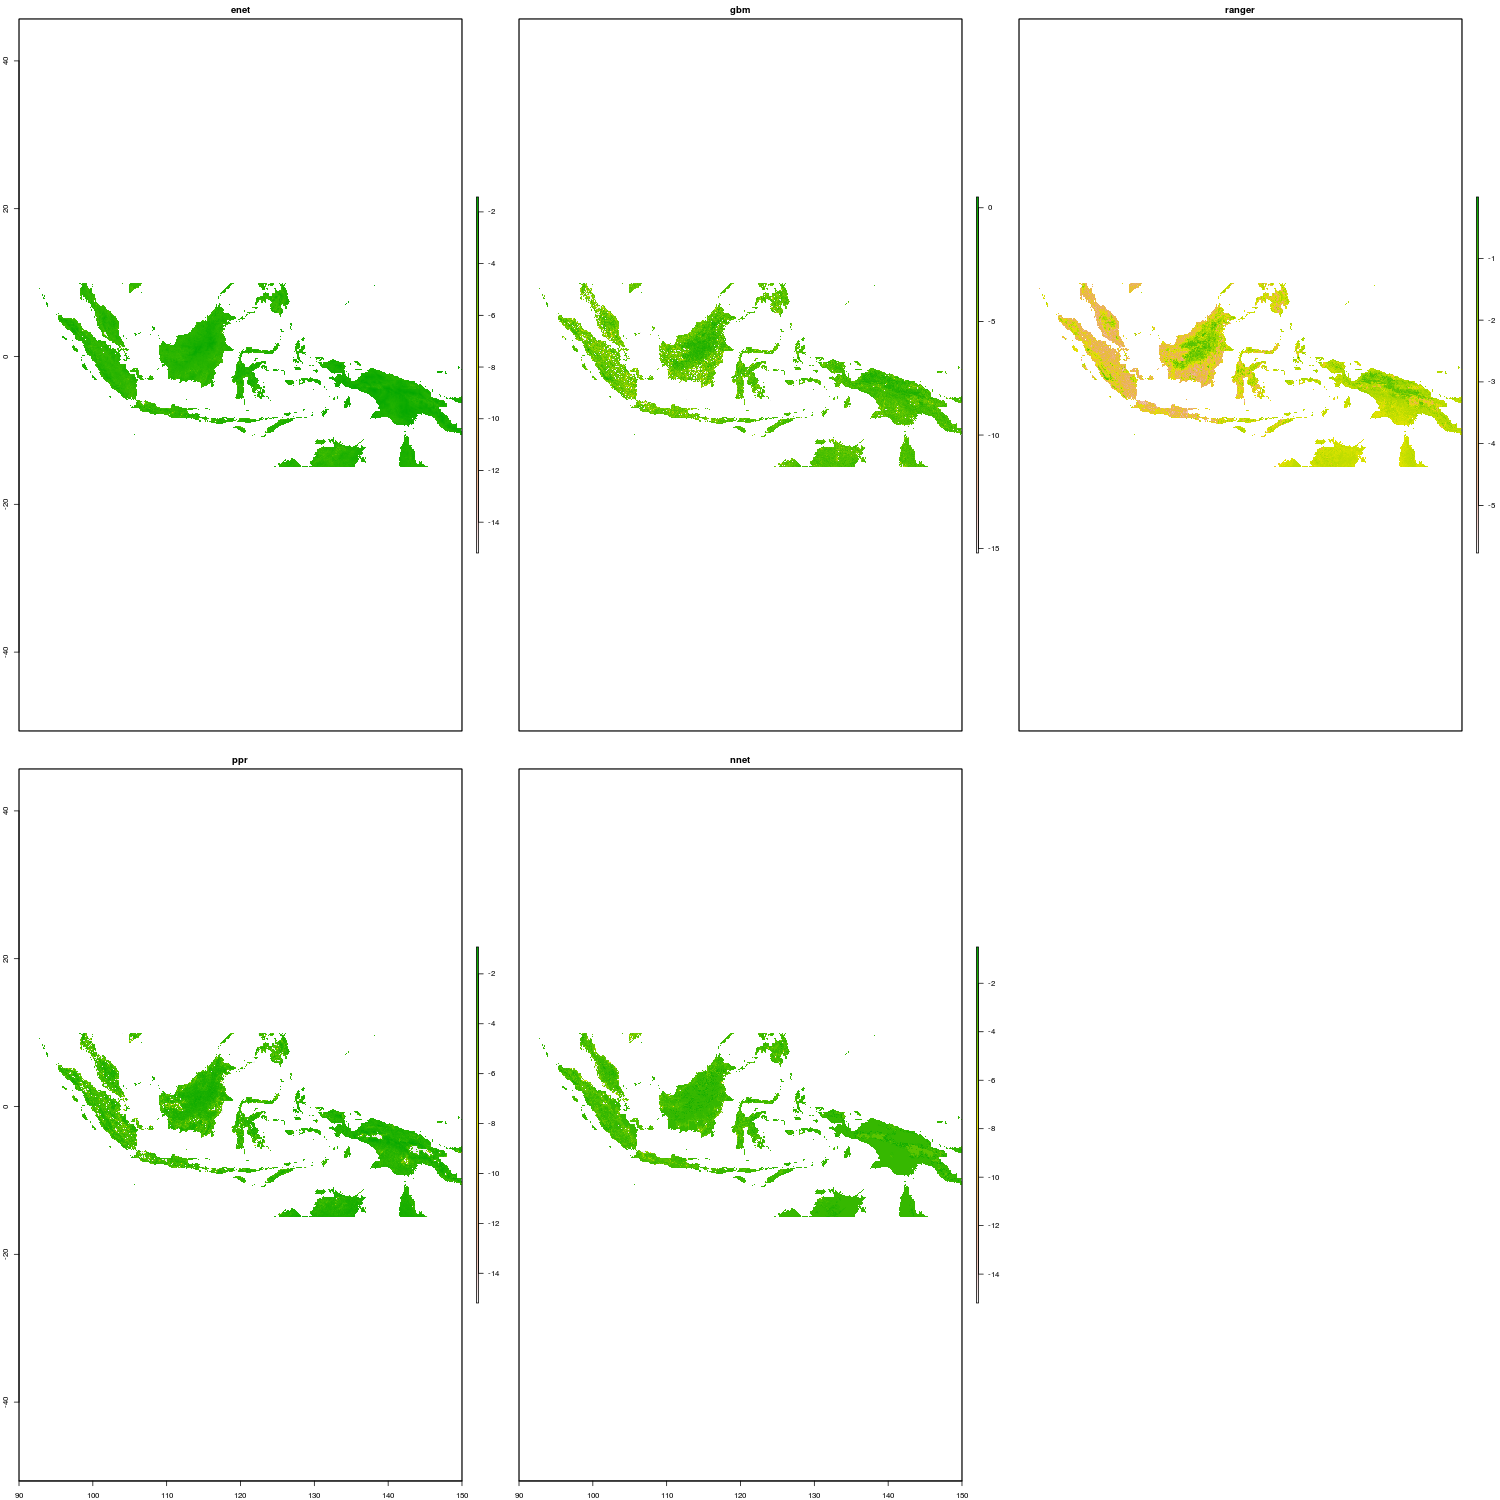
\includegraphics[width=1\textwidth]{figs/SI/idn_all_ml.png}
\caption{
  Predictions from machine learning models trained on Indonesian prevalence data.
}

\end{figure}


\begin{figure}[h!]
  \centering
  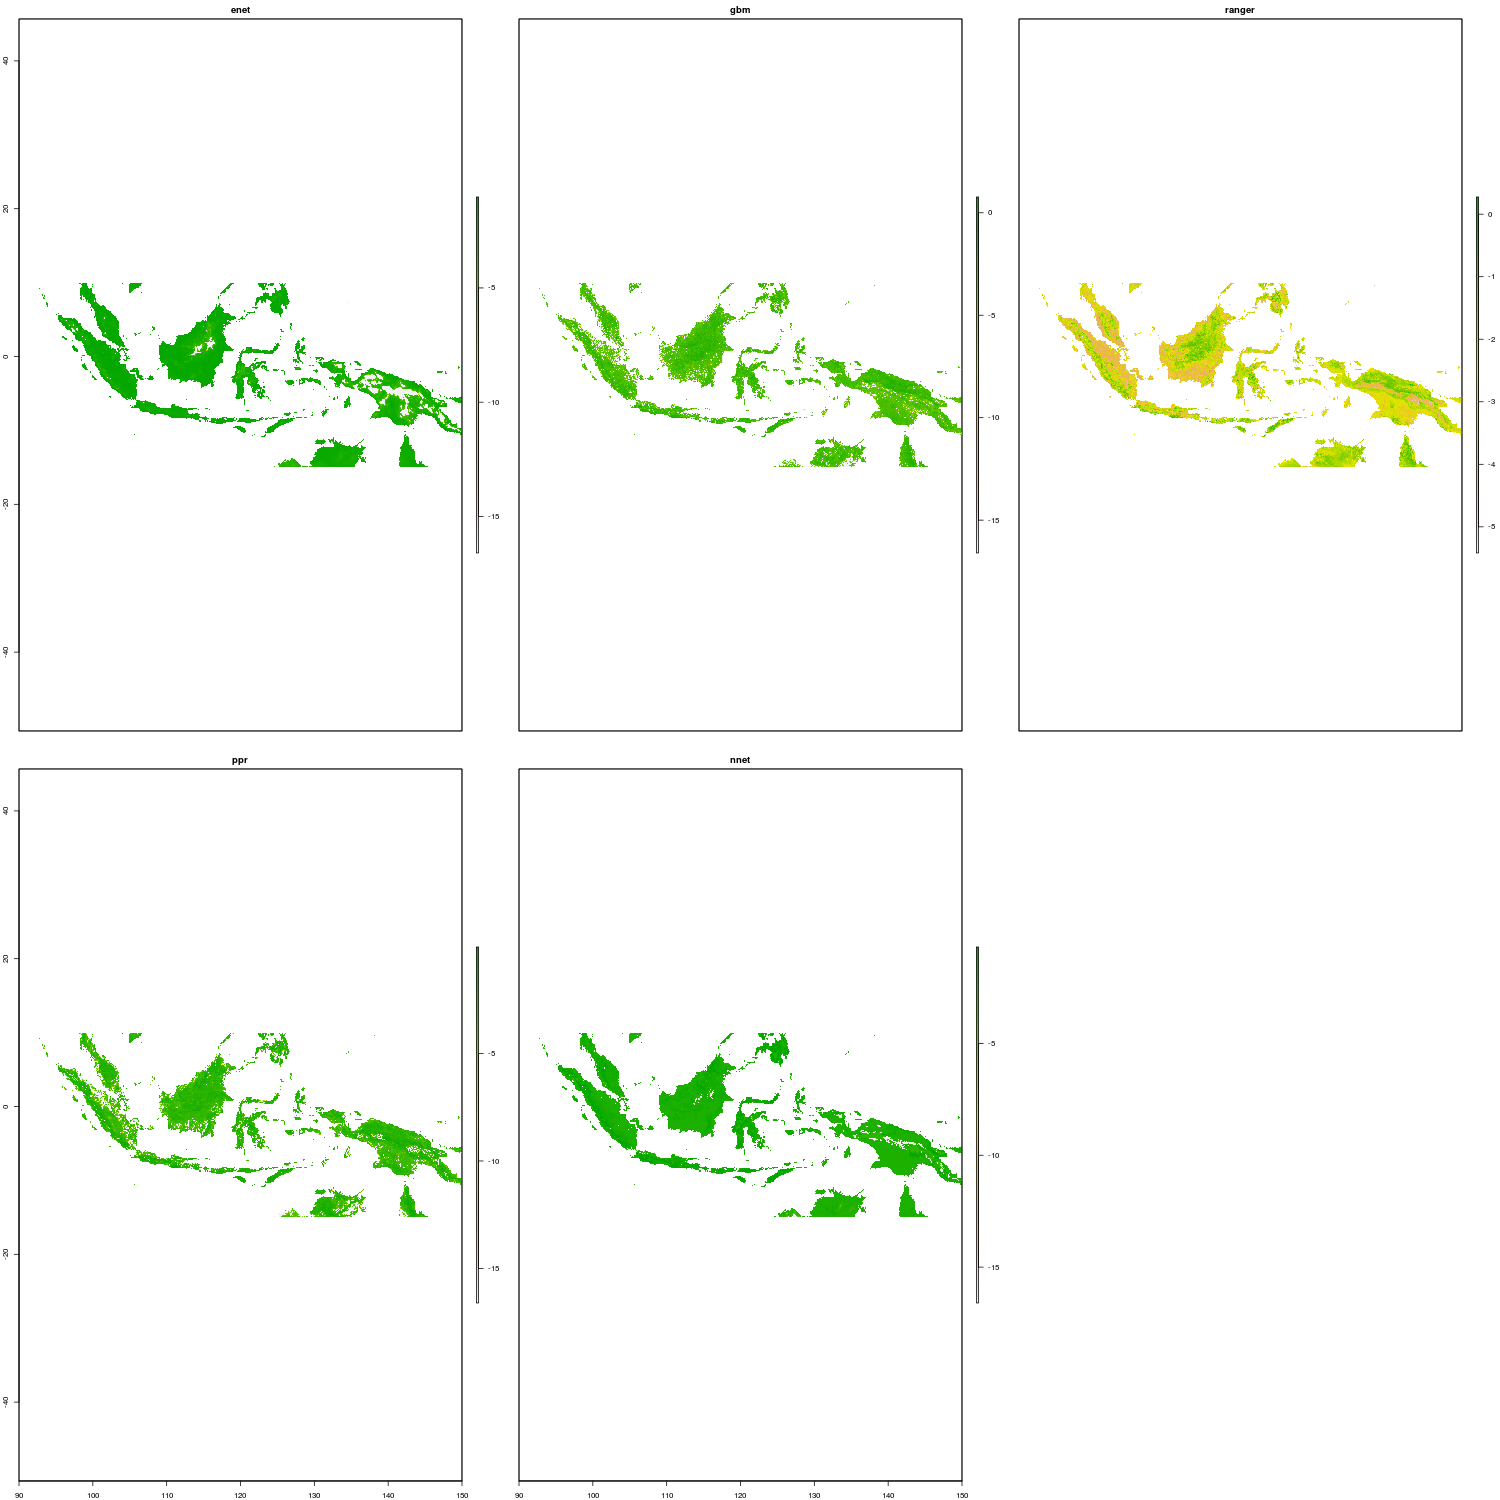
\includegraphics[width=1\textwidth]{figs/SI/idn_all_globalml.png}
\caption{
  Predictions over Indonesia from machine learning models trained on global prevalence data.
}

\end{figure}




\clearpage
\subsection{Out-of-sample scatter plots}


\begin{figure}[h!]
  \centering
  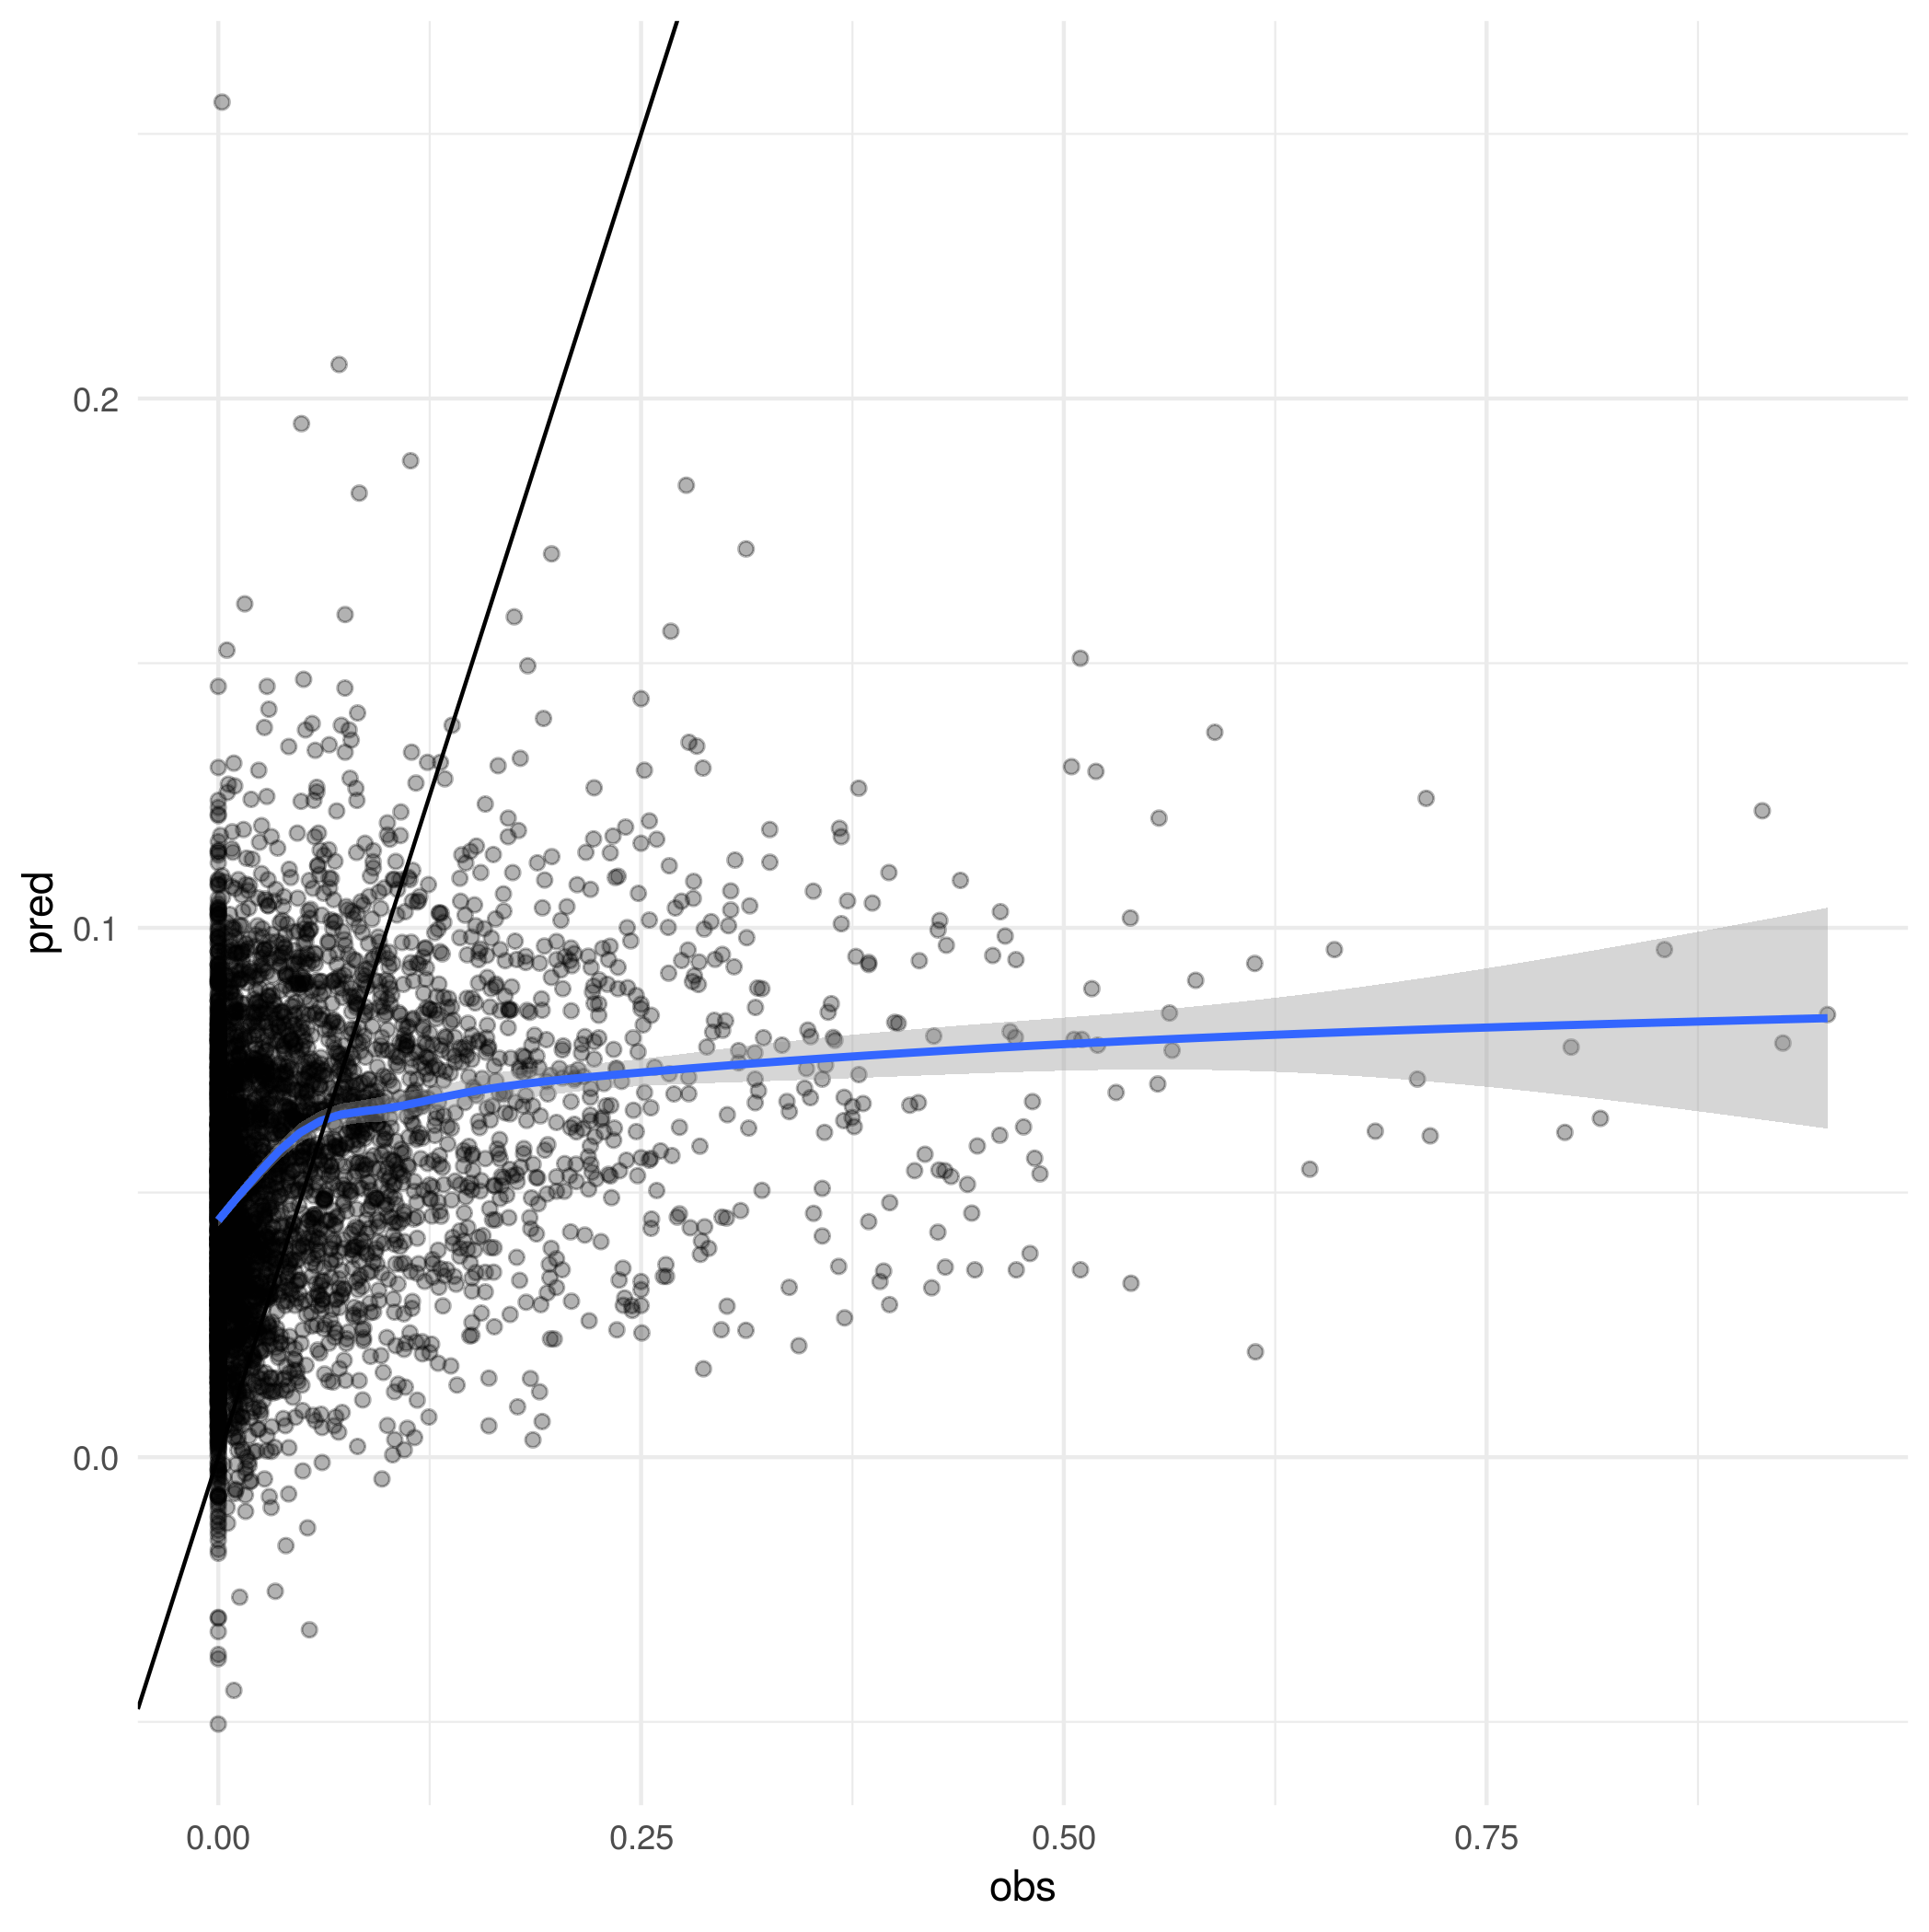
\includegraphics[width=0.6\textwidth]{figs/SI/nnet_obspred_idn.png}
\caption{
  Scatter plot of predictions and held out observed data for the neural network trained on the Indonesia dataset.
}

\end{figure}



\begin{figure}[h!]
  \centering
  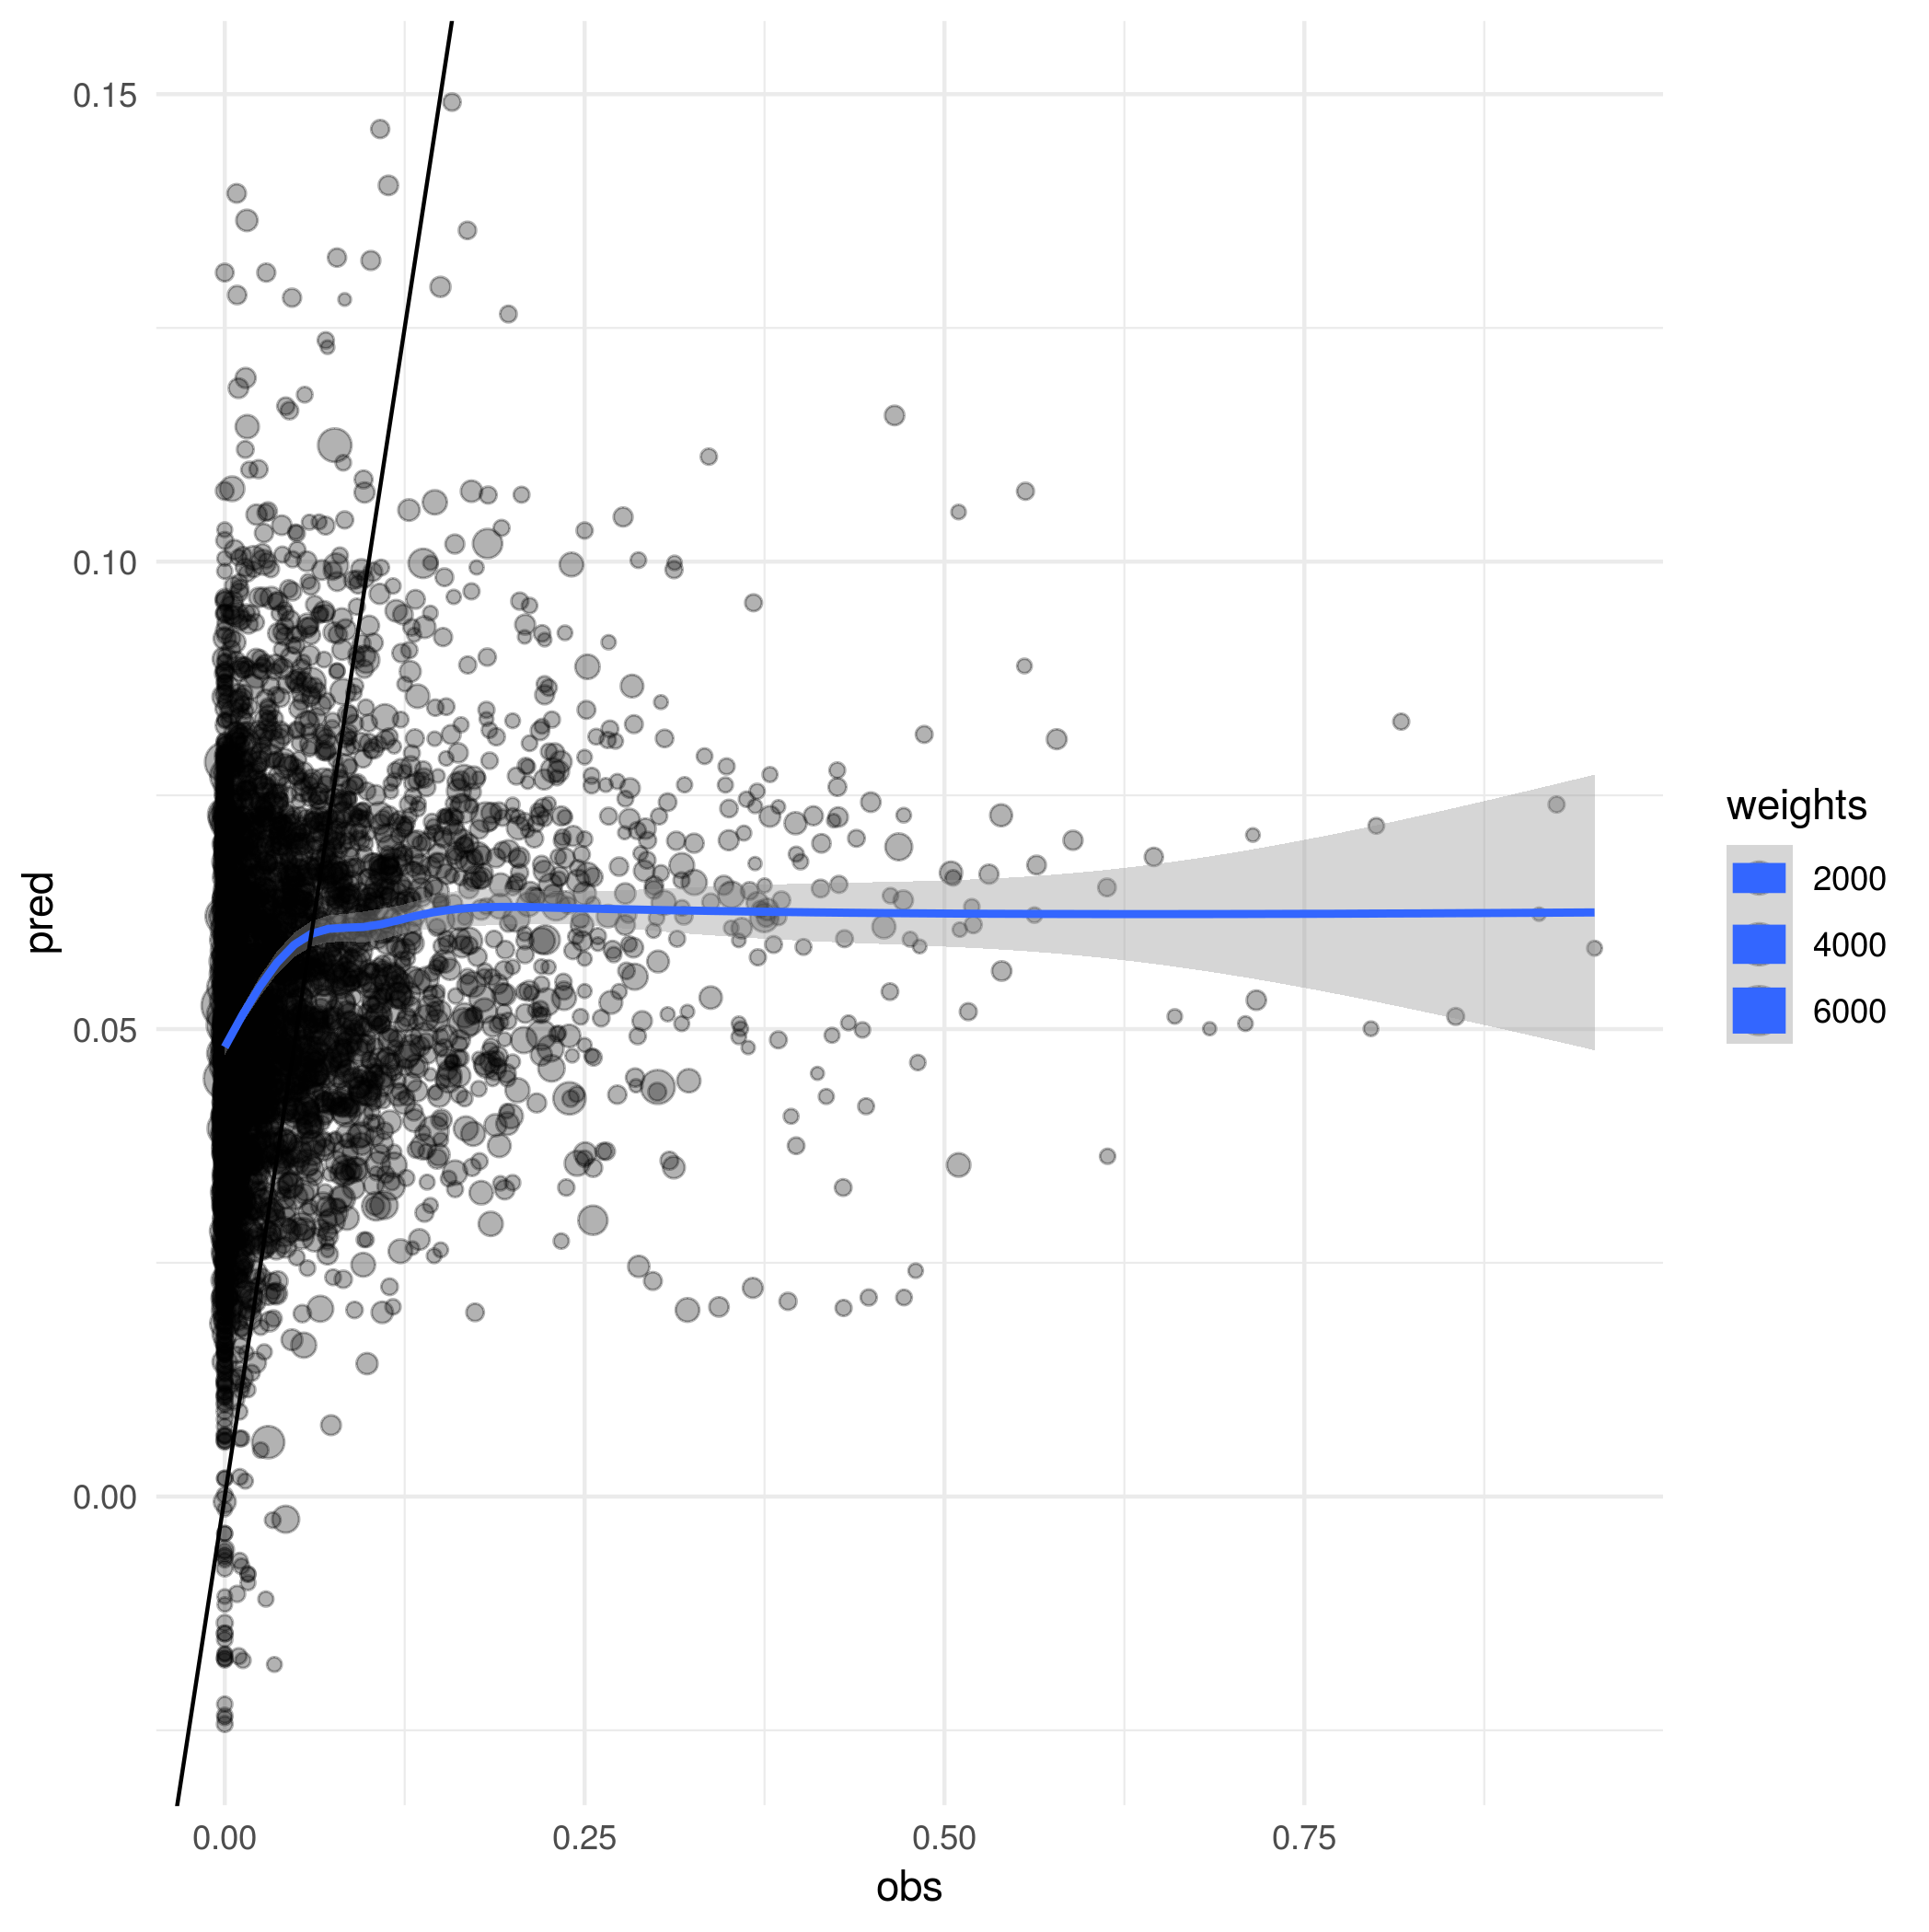
\includegraphics[width=0.6\textwidth]{figs/SI/enet_obspred_idn.png}
\caption{
  Scatter plot of predictions and held out observed data for the elastic net trained on the Indonesia dataset.
}

\end{figure}


\begin{figure}[h!]
  \centering
  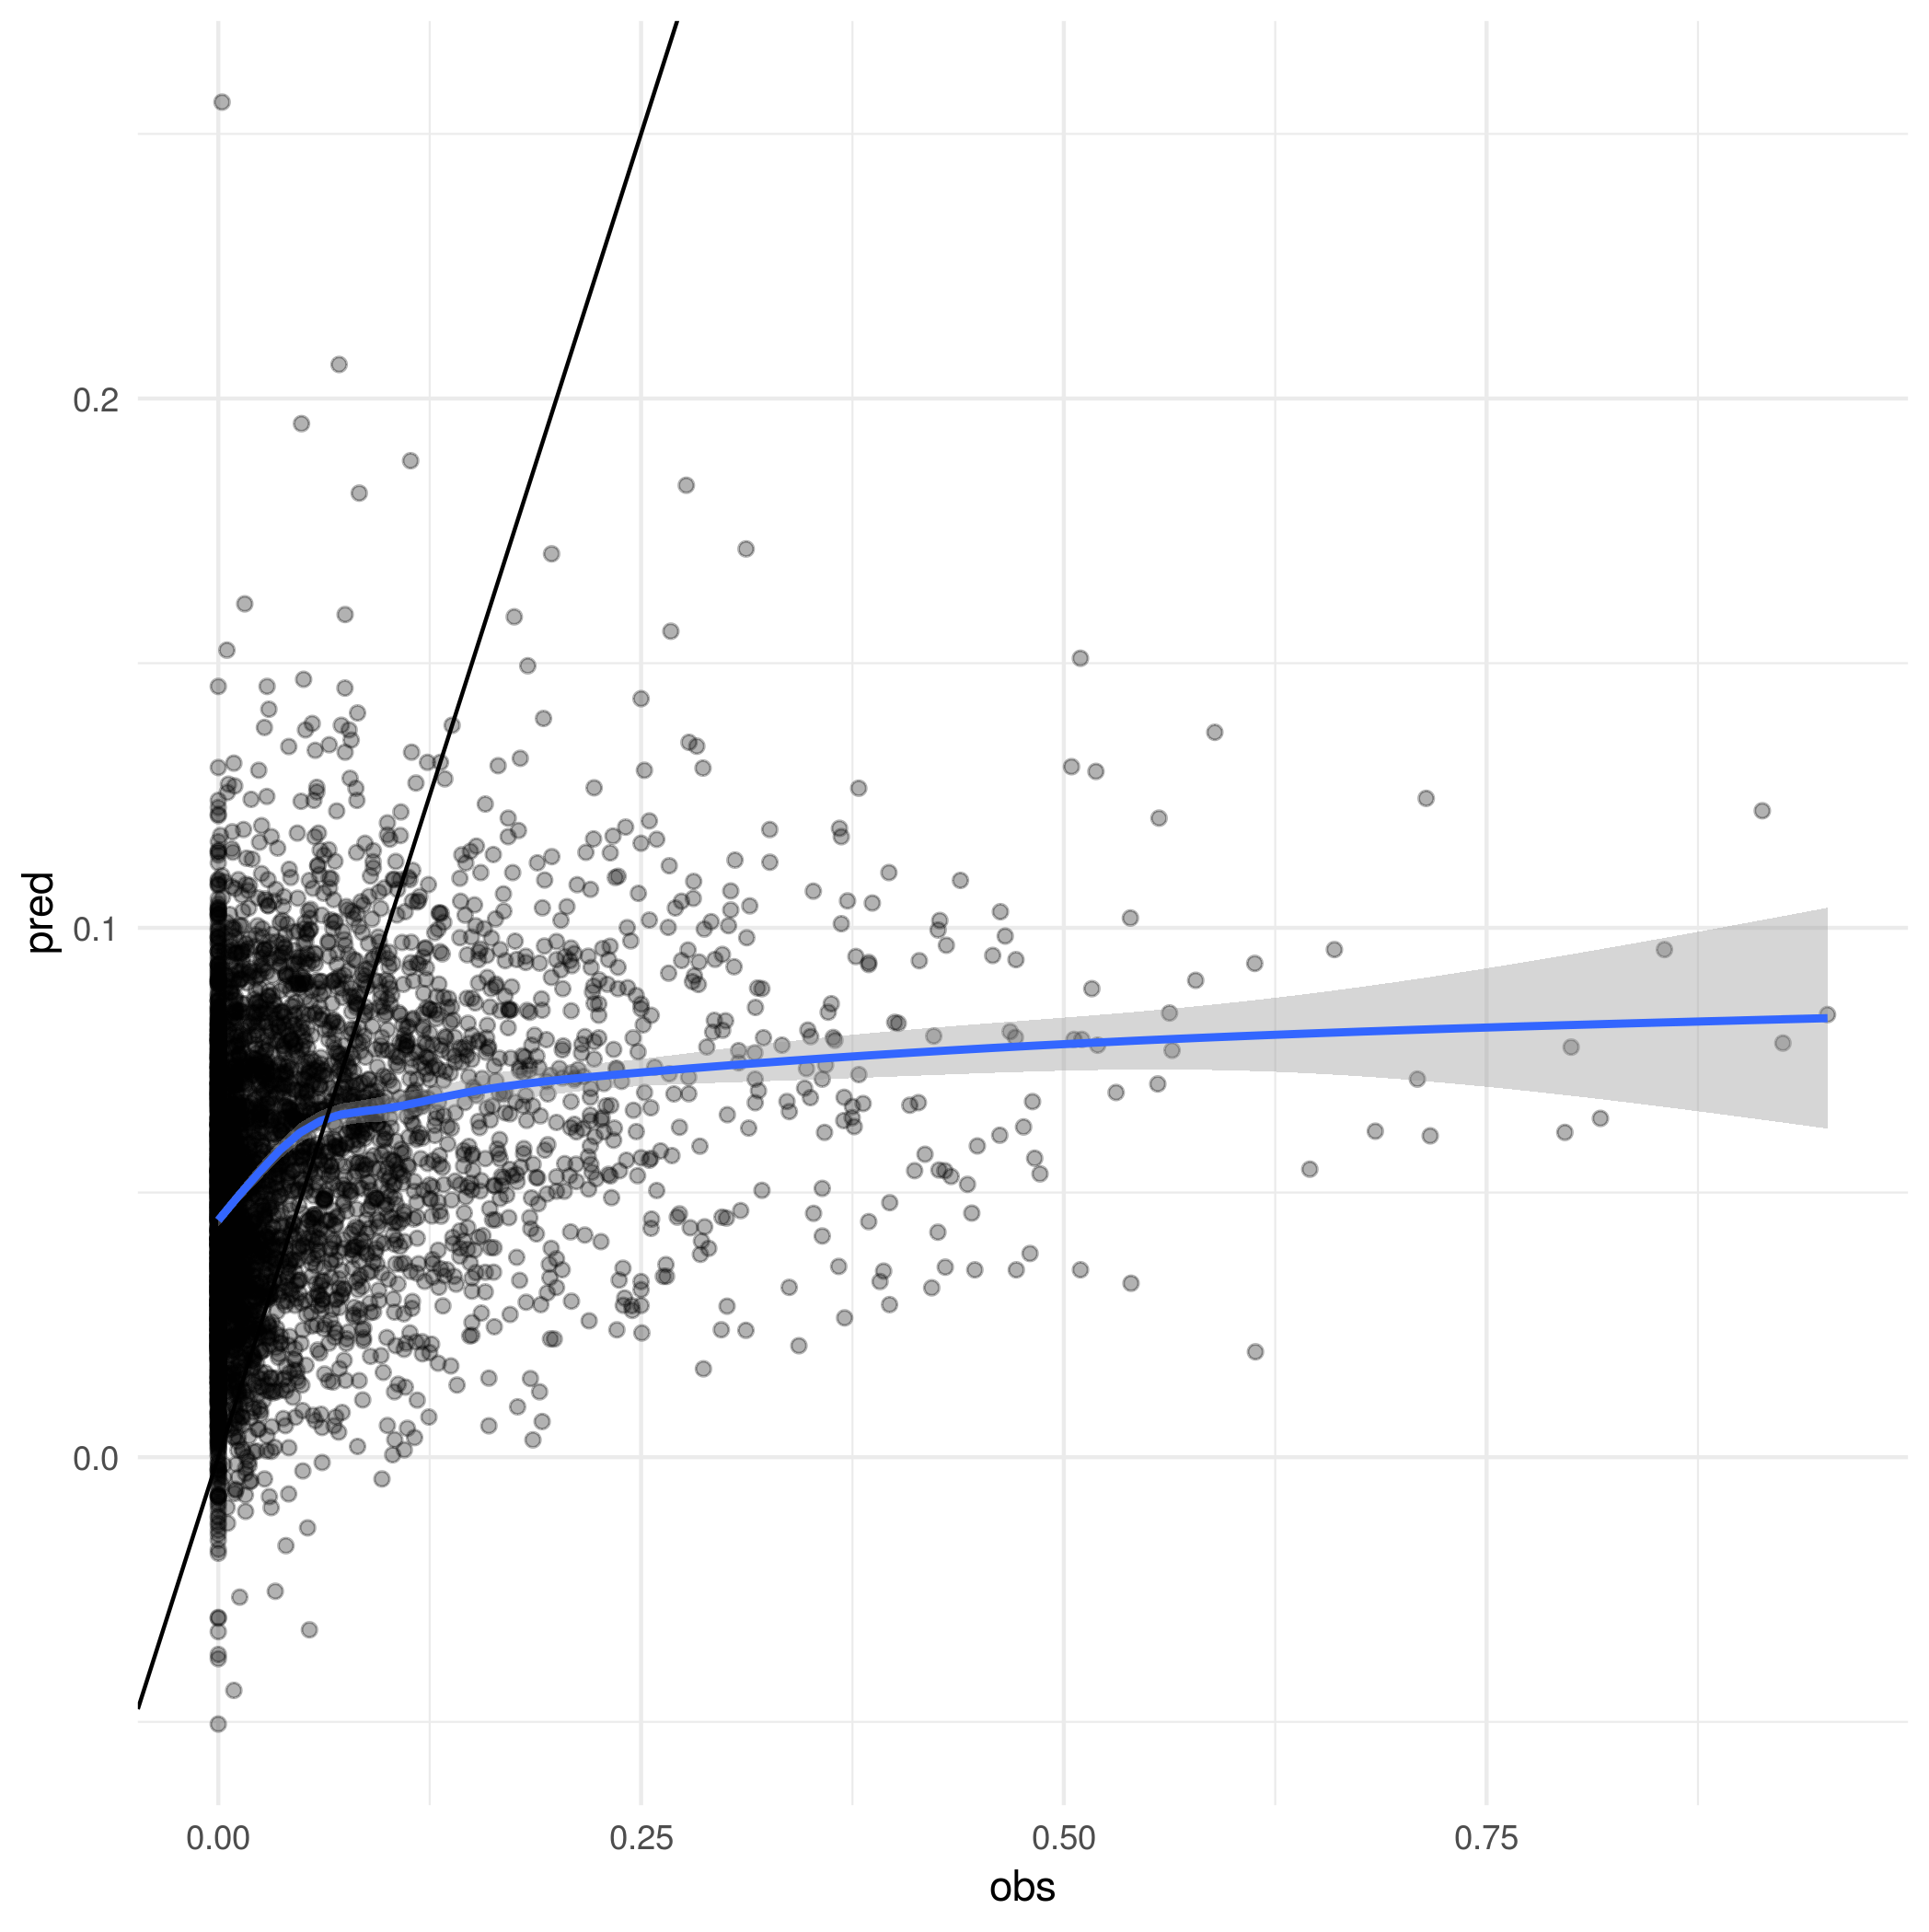
\includegraphics[width=0.6\textwidth]{figs/SI/ppr_obspred_idn.png}
\caption{
  Scatter plot of predictions and held out observed data for the PPR trained on the Indonesia dataset.
}

\end{figure}


\begin{figure}[h!]
  \centering
  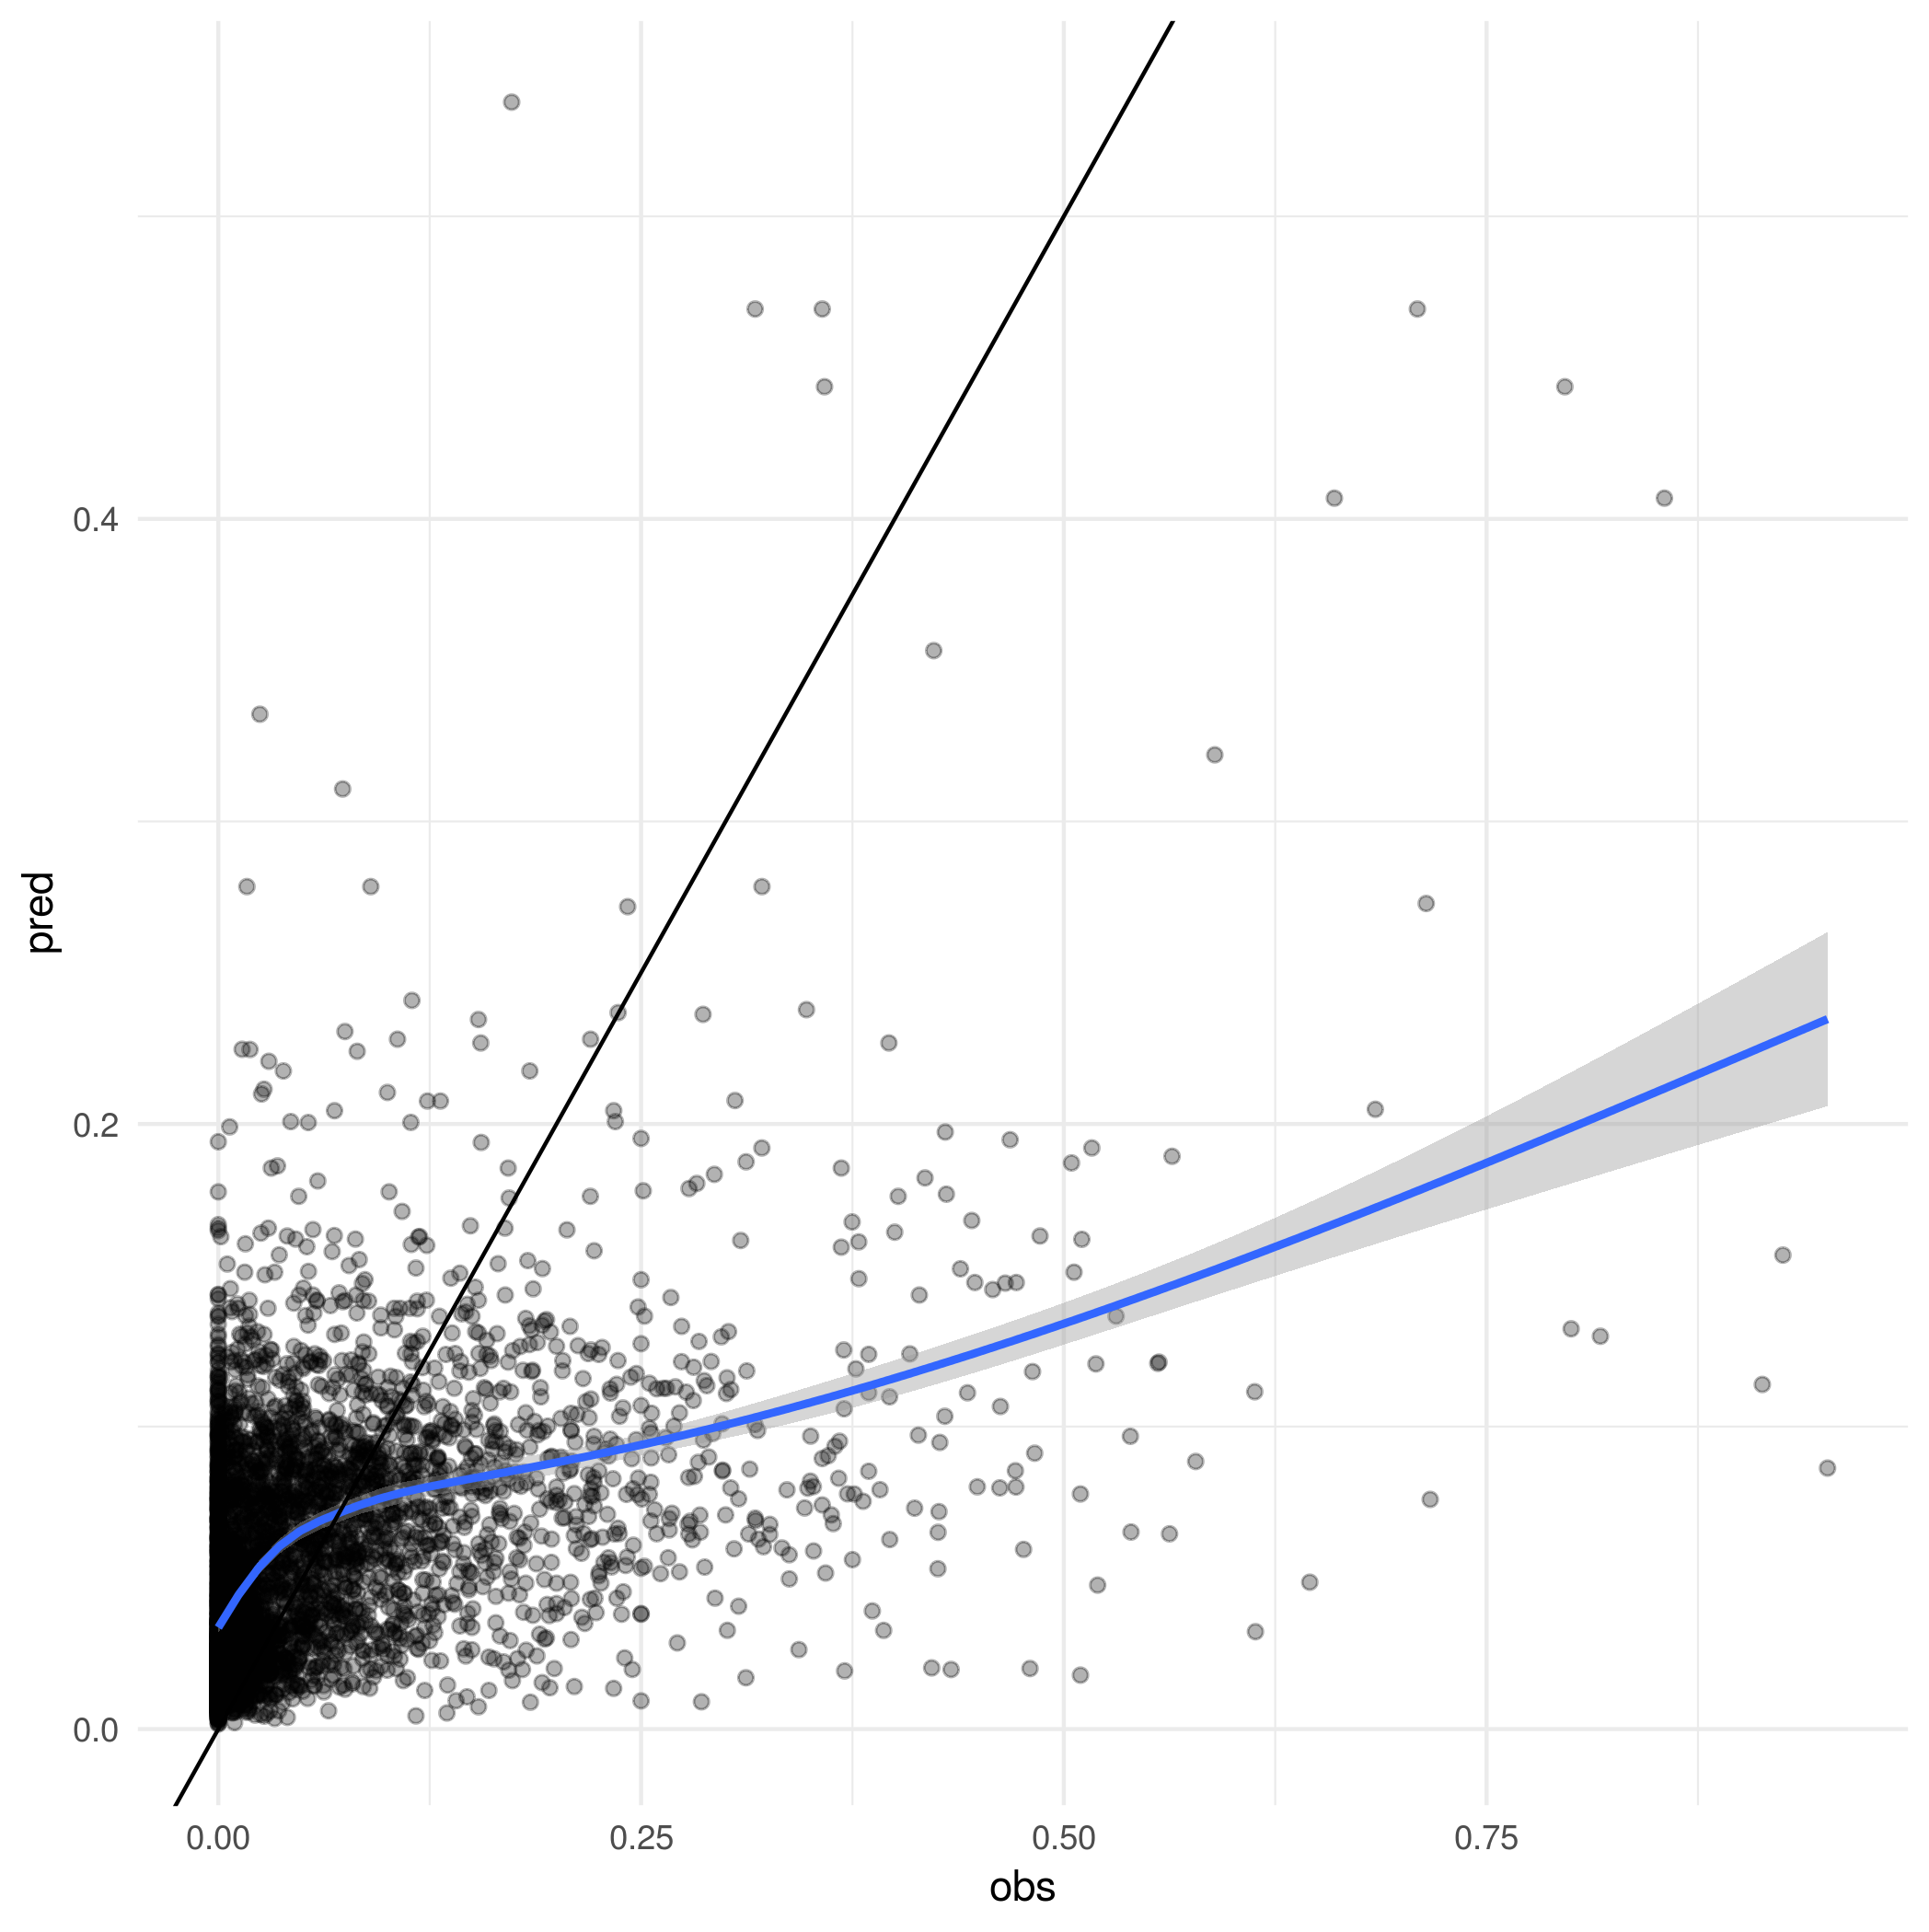
\includegraphics[width=0.6\textwidth]{figs/SI/ranger_obspred_idn.png}
\caption{
  Scatter plot of predictions and held out observed data for the Random Forest trained on the Indonesia dataset.
}

\end{figure}


\begin{figure}[h!]
  \centering
  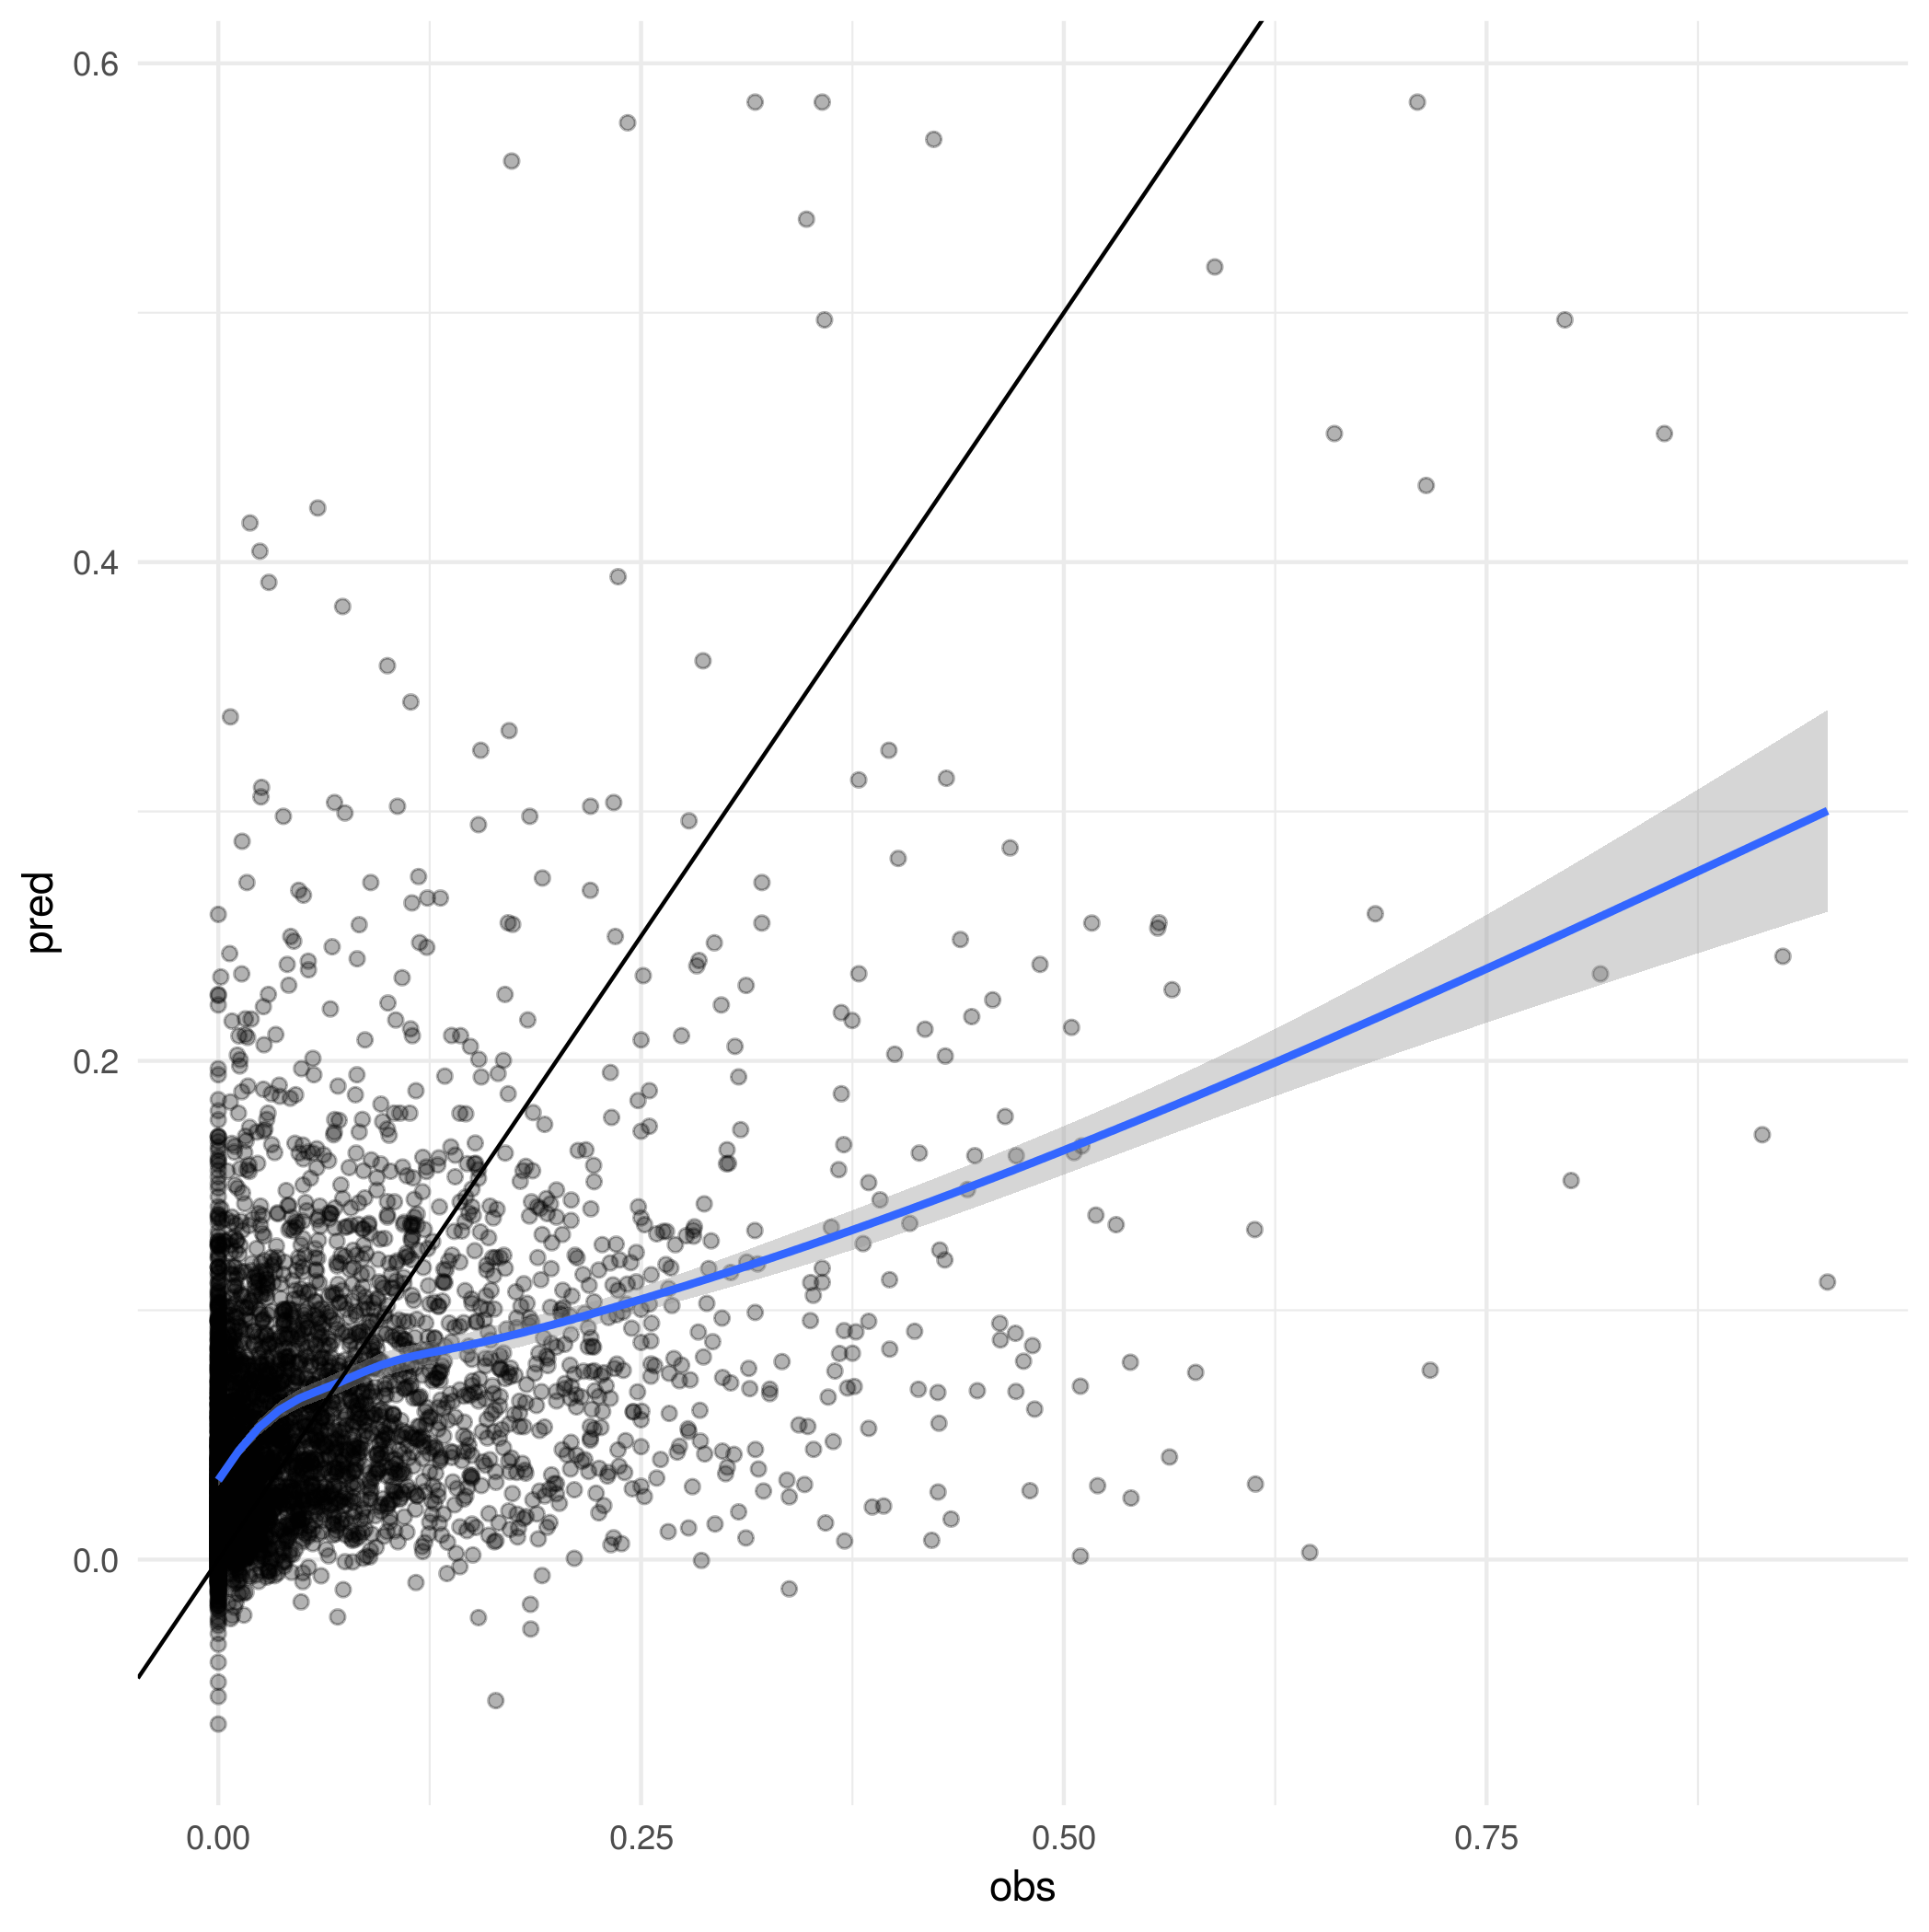
\includegraphics[width=0.6\textwidth]{figs/SI/xgboost_obspred_idn.png}
\caption{
  Scatter plot of predictions and held out observed data for the GBM trained on the Indonesia dataset.
}

\end{figure}


\clearpage
\subsection{Hyperparameter optimisation}

As ranger and GBM were tuned with random hyperparameter search, the plots become difficult and are not included.


\begin{figure}[h!]
  \centering
  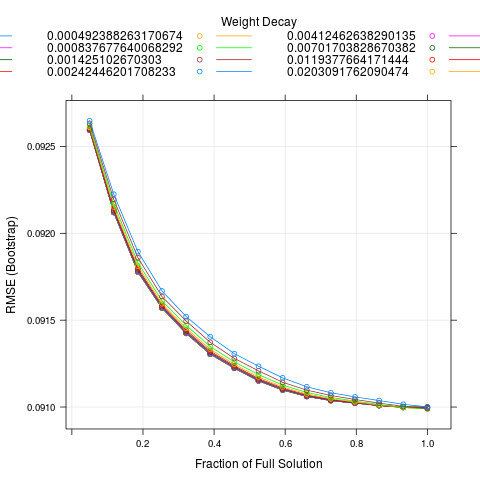
\includegraphics[width=0.6\textwidth]{figs/SI/enetopt_idn.png}
\caption{
  Optimisation for elastic net hyperparameters trained on the Indonesia dataset.
}
\end{figure}



\begin{figure}[h!]
  \centering
  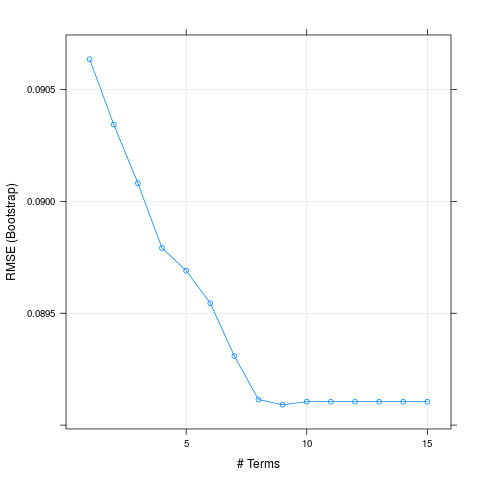
\includegraphics[width=0.6\textwidth]{figs/SI/ppropt_idn.png}
\caption{
  Optimisation for PPR hyperparameters trained on the Indonesia dataset.
}

\end{figure}






\clearpage
%%%%%%%%%%%%%%%%%%%%%%%%%%%%%%%%%%%%%%%%%%%%%%%%%%%%%%%%%%%%%%%%%%%%%%%
\section{Madagascar dataset Machine Learning}
%%%%%%%%%%%%%%%%%%%%%%%%%%%%%%%%%%%%%%%%%%%%%%%%%%%%%%%%%%%%%%%%%%%%%%%





\subsection{Predictions}

\begin{figure}[h!]
  \centering
  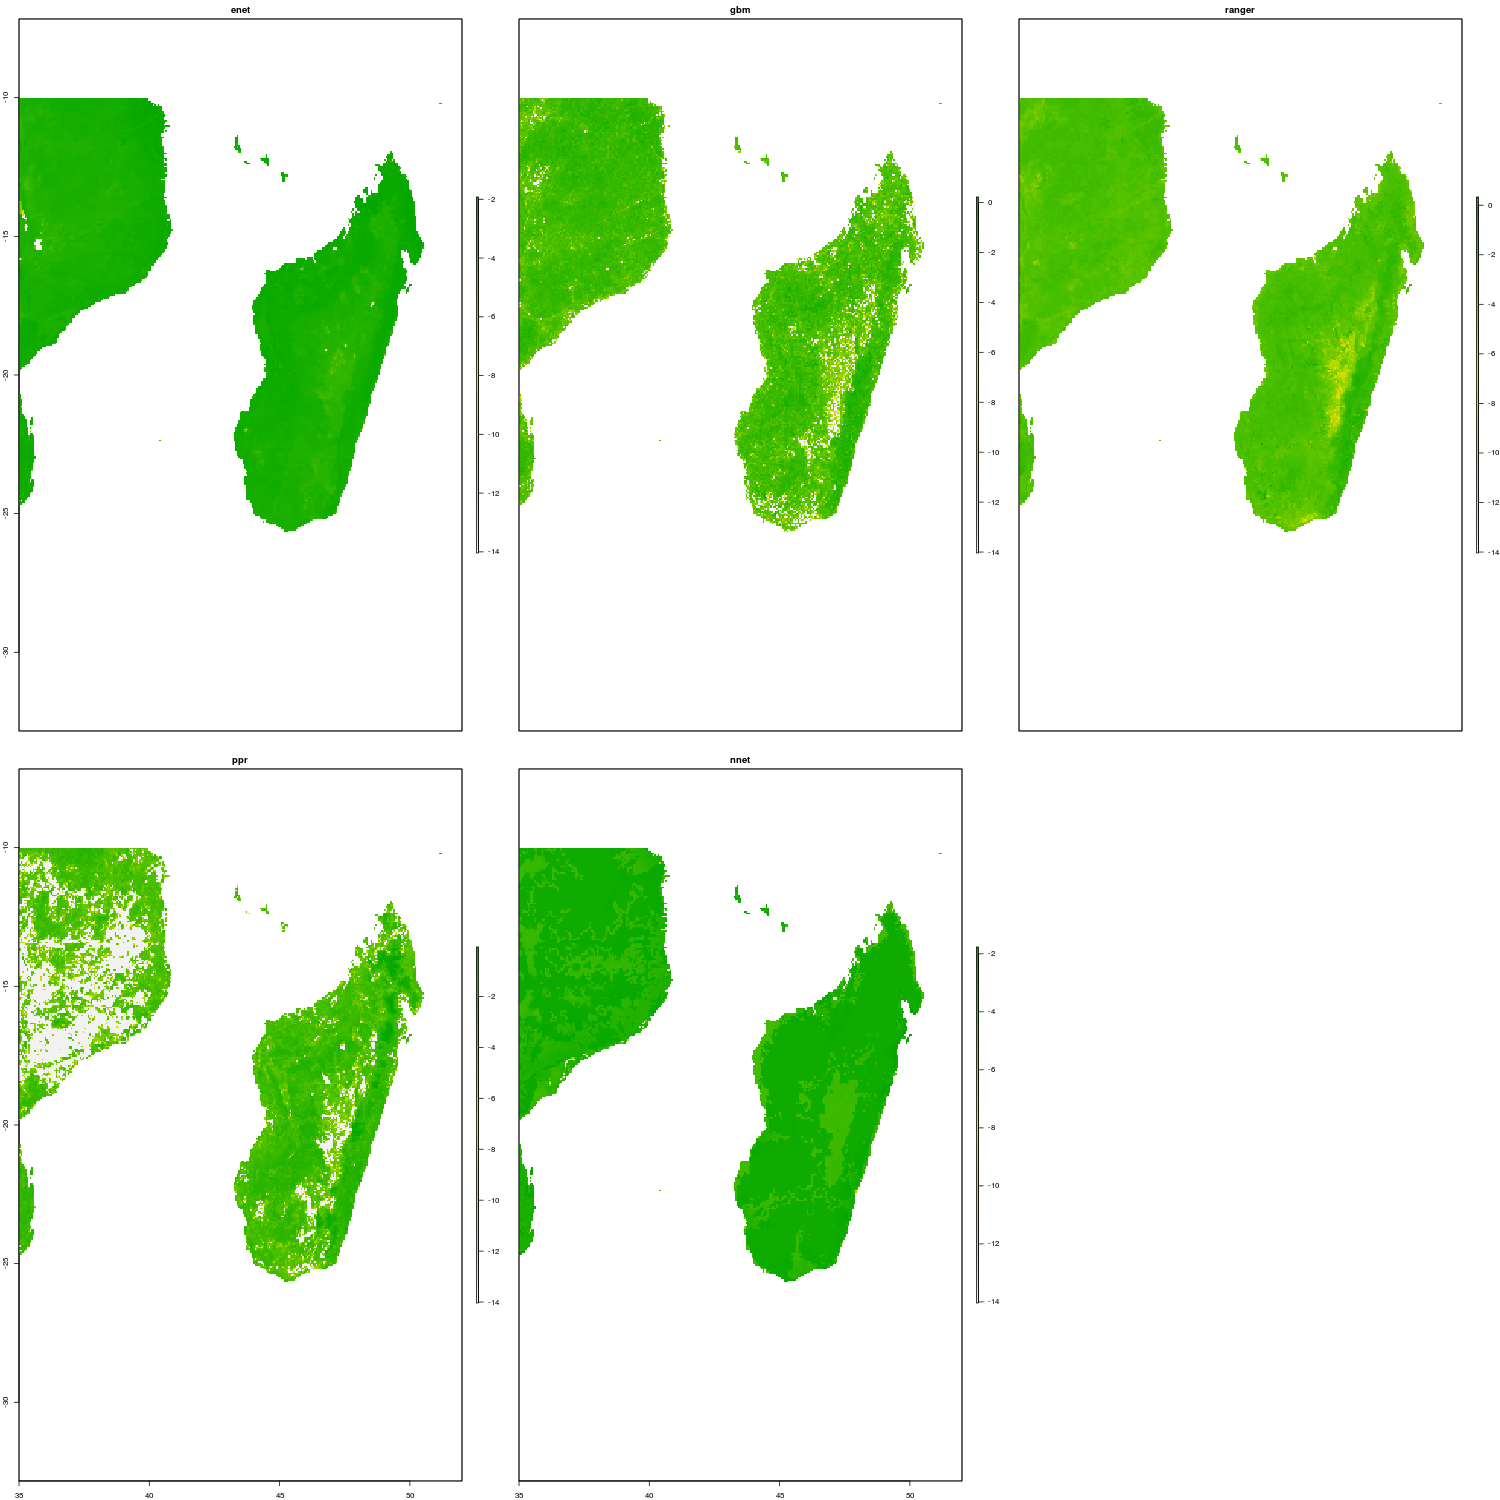
\includegraphics[width=1\textwidth]{figs/SI/MDG_all_ml.png}
\caption{
  Predictions from machine learning models trained on Malagasy prevalence data.
}

\end{figure}


\begin{figure}[h!]
  \centering
  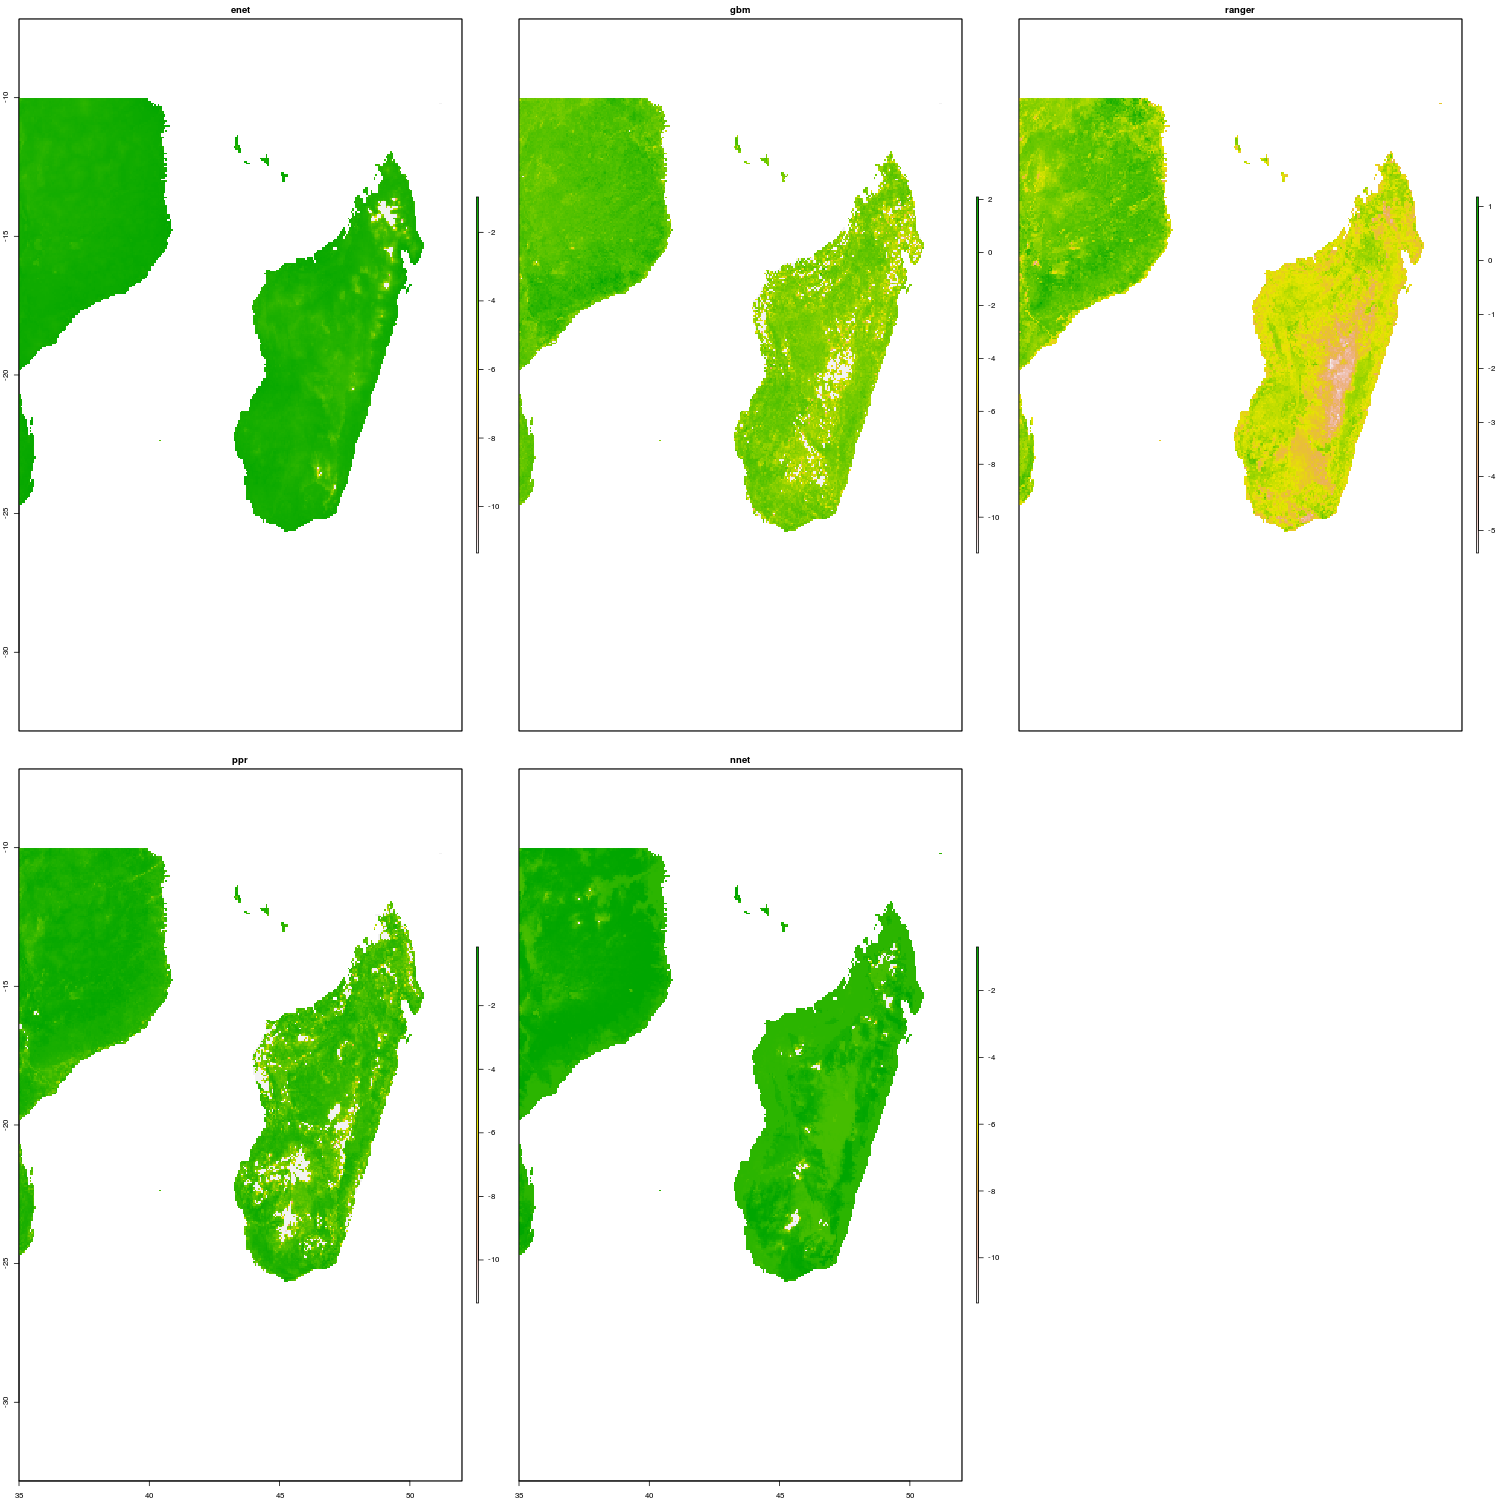
\includegraphics[width=1\textwidth]{figs/SI/MDG_all_globalml.png}
\caption{
  Predictions over Madagascar from machine learning models trained on global prevalence data.
}

\end{figure}




\clearpage
\subsection{Out-of-sample scatter plots}


\begin{figure}[h!]
  \centering
  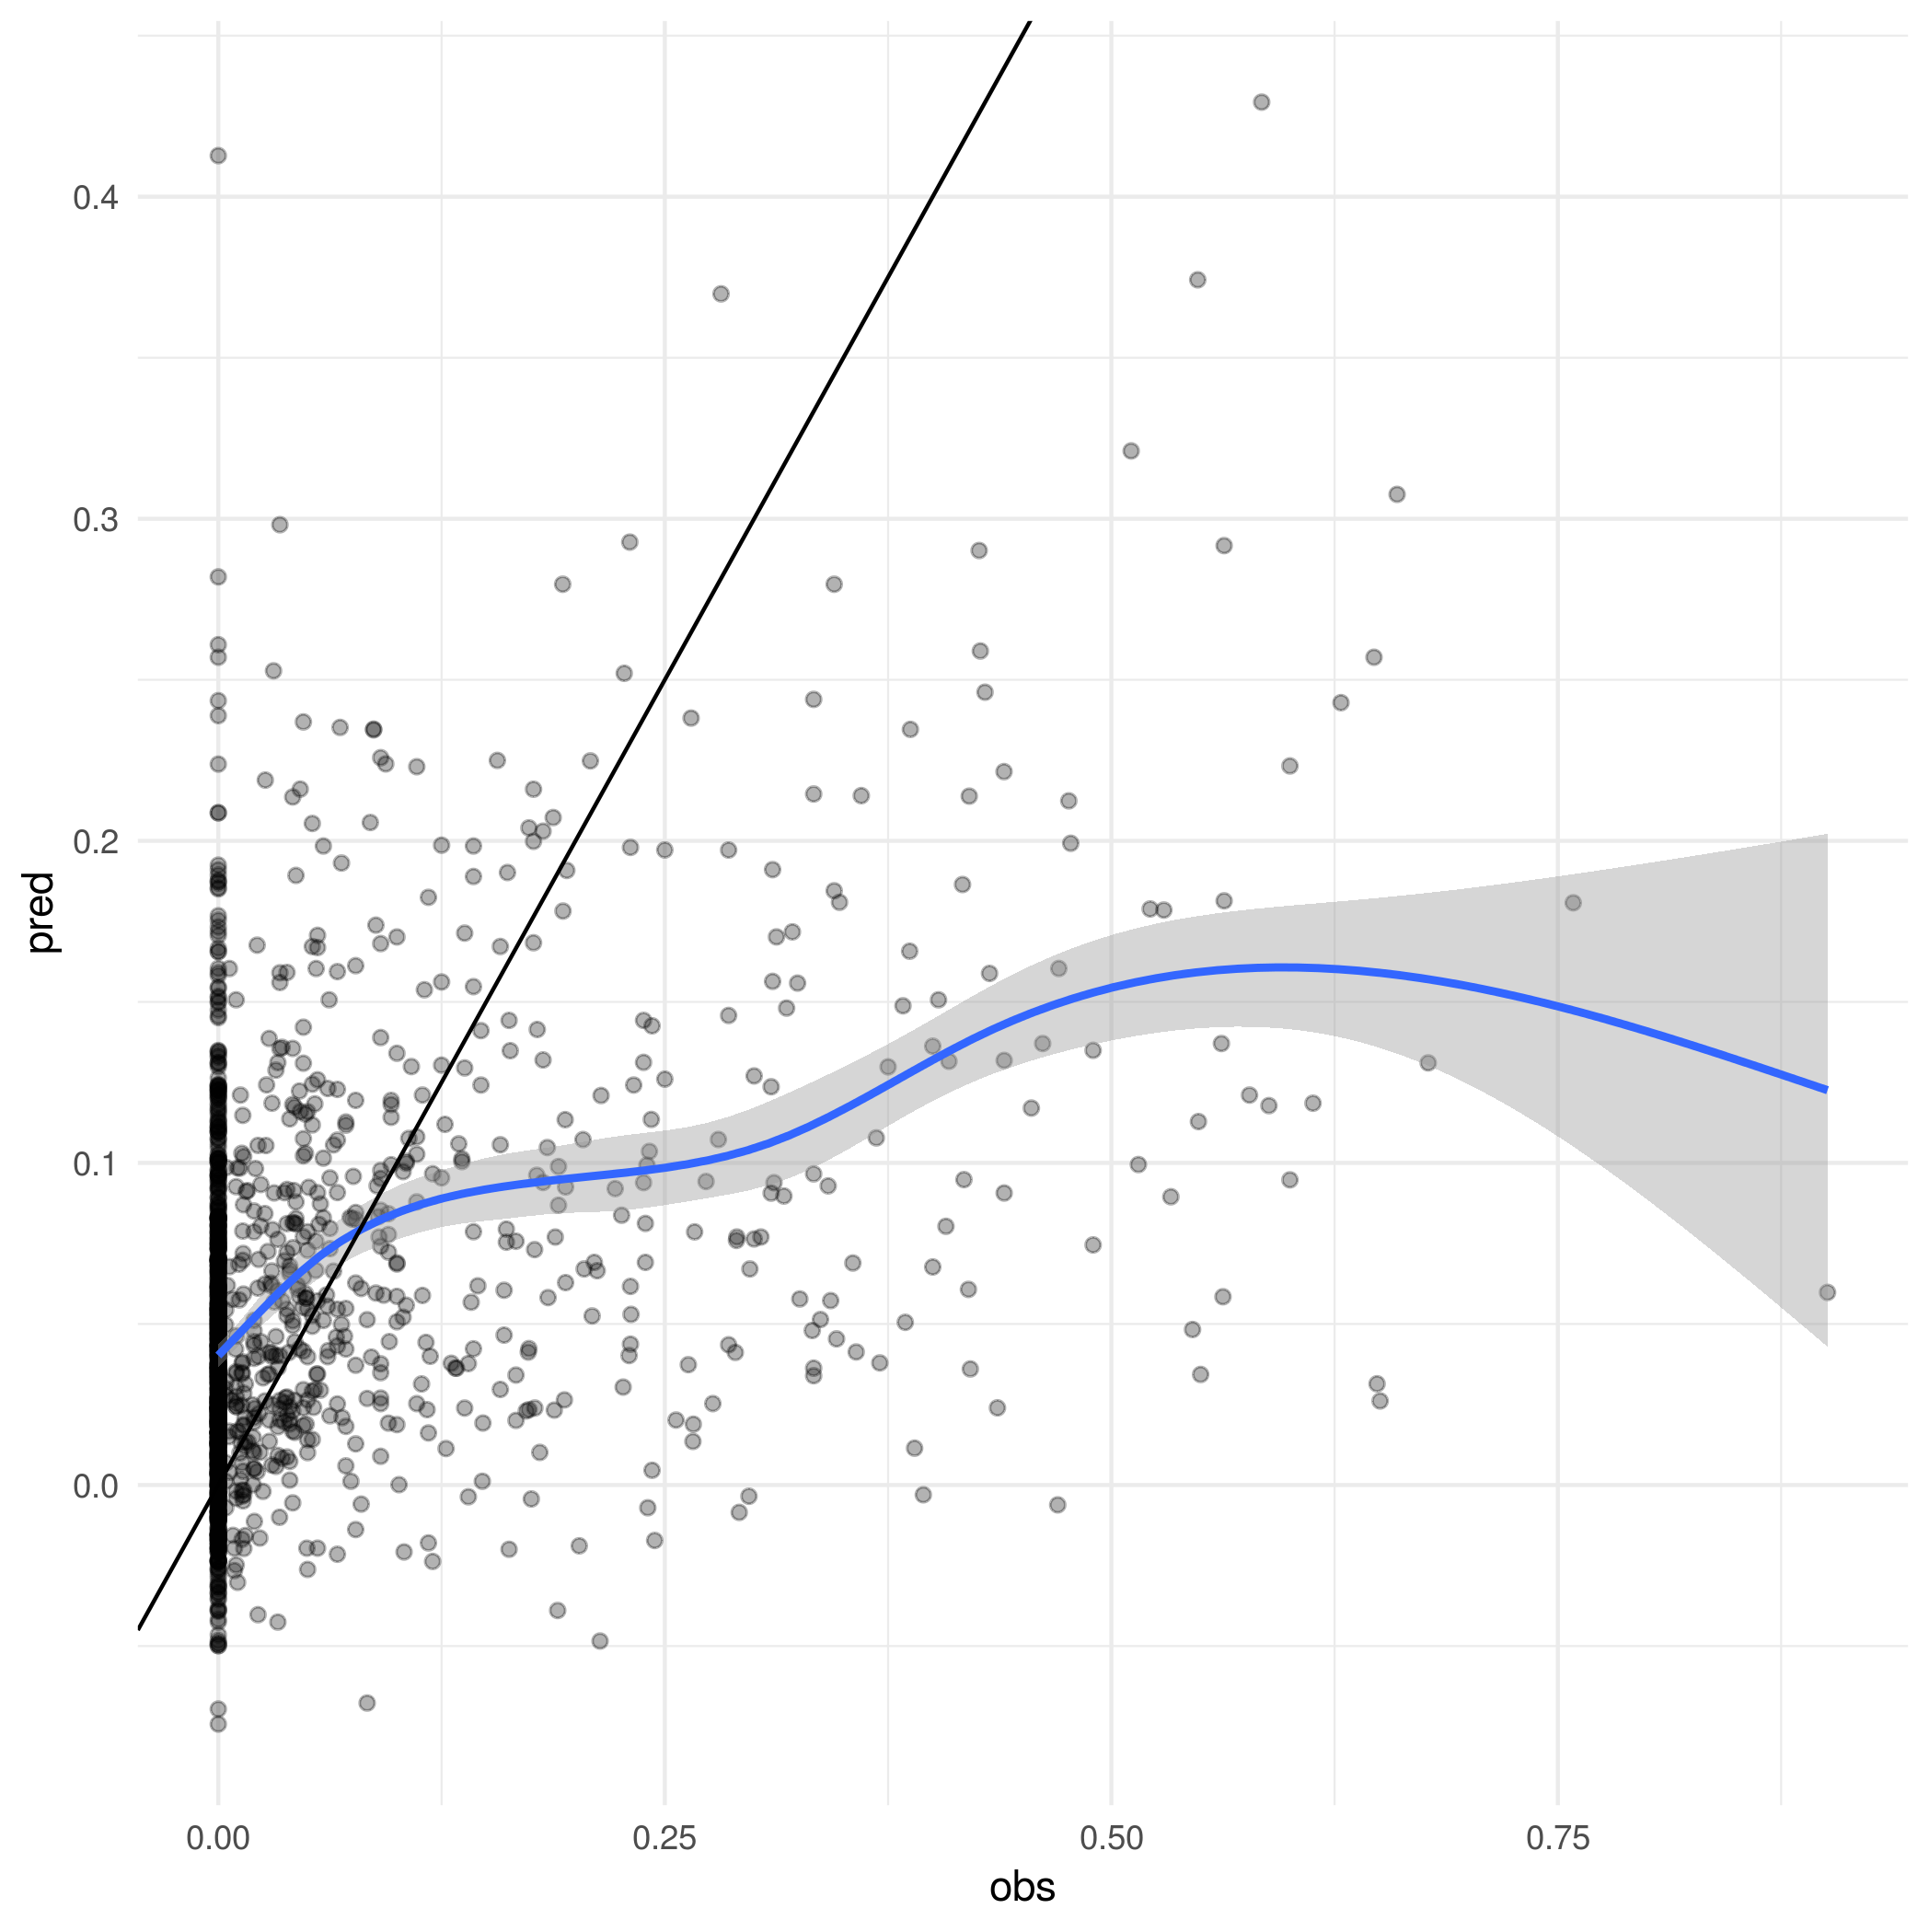
\includegraphics[width=0.6\textwidth]{figs/SI/nnet_obspred_mdg.png}
\caption{
  Scatter plot of predictions and held out observed data for the neural network trained on the Madagascar dataset.
}

\end{figure}



\begin{figure}[h!]
  \centering
  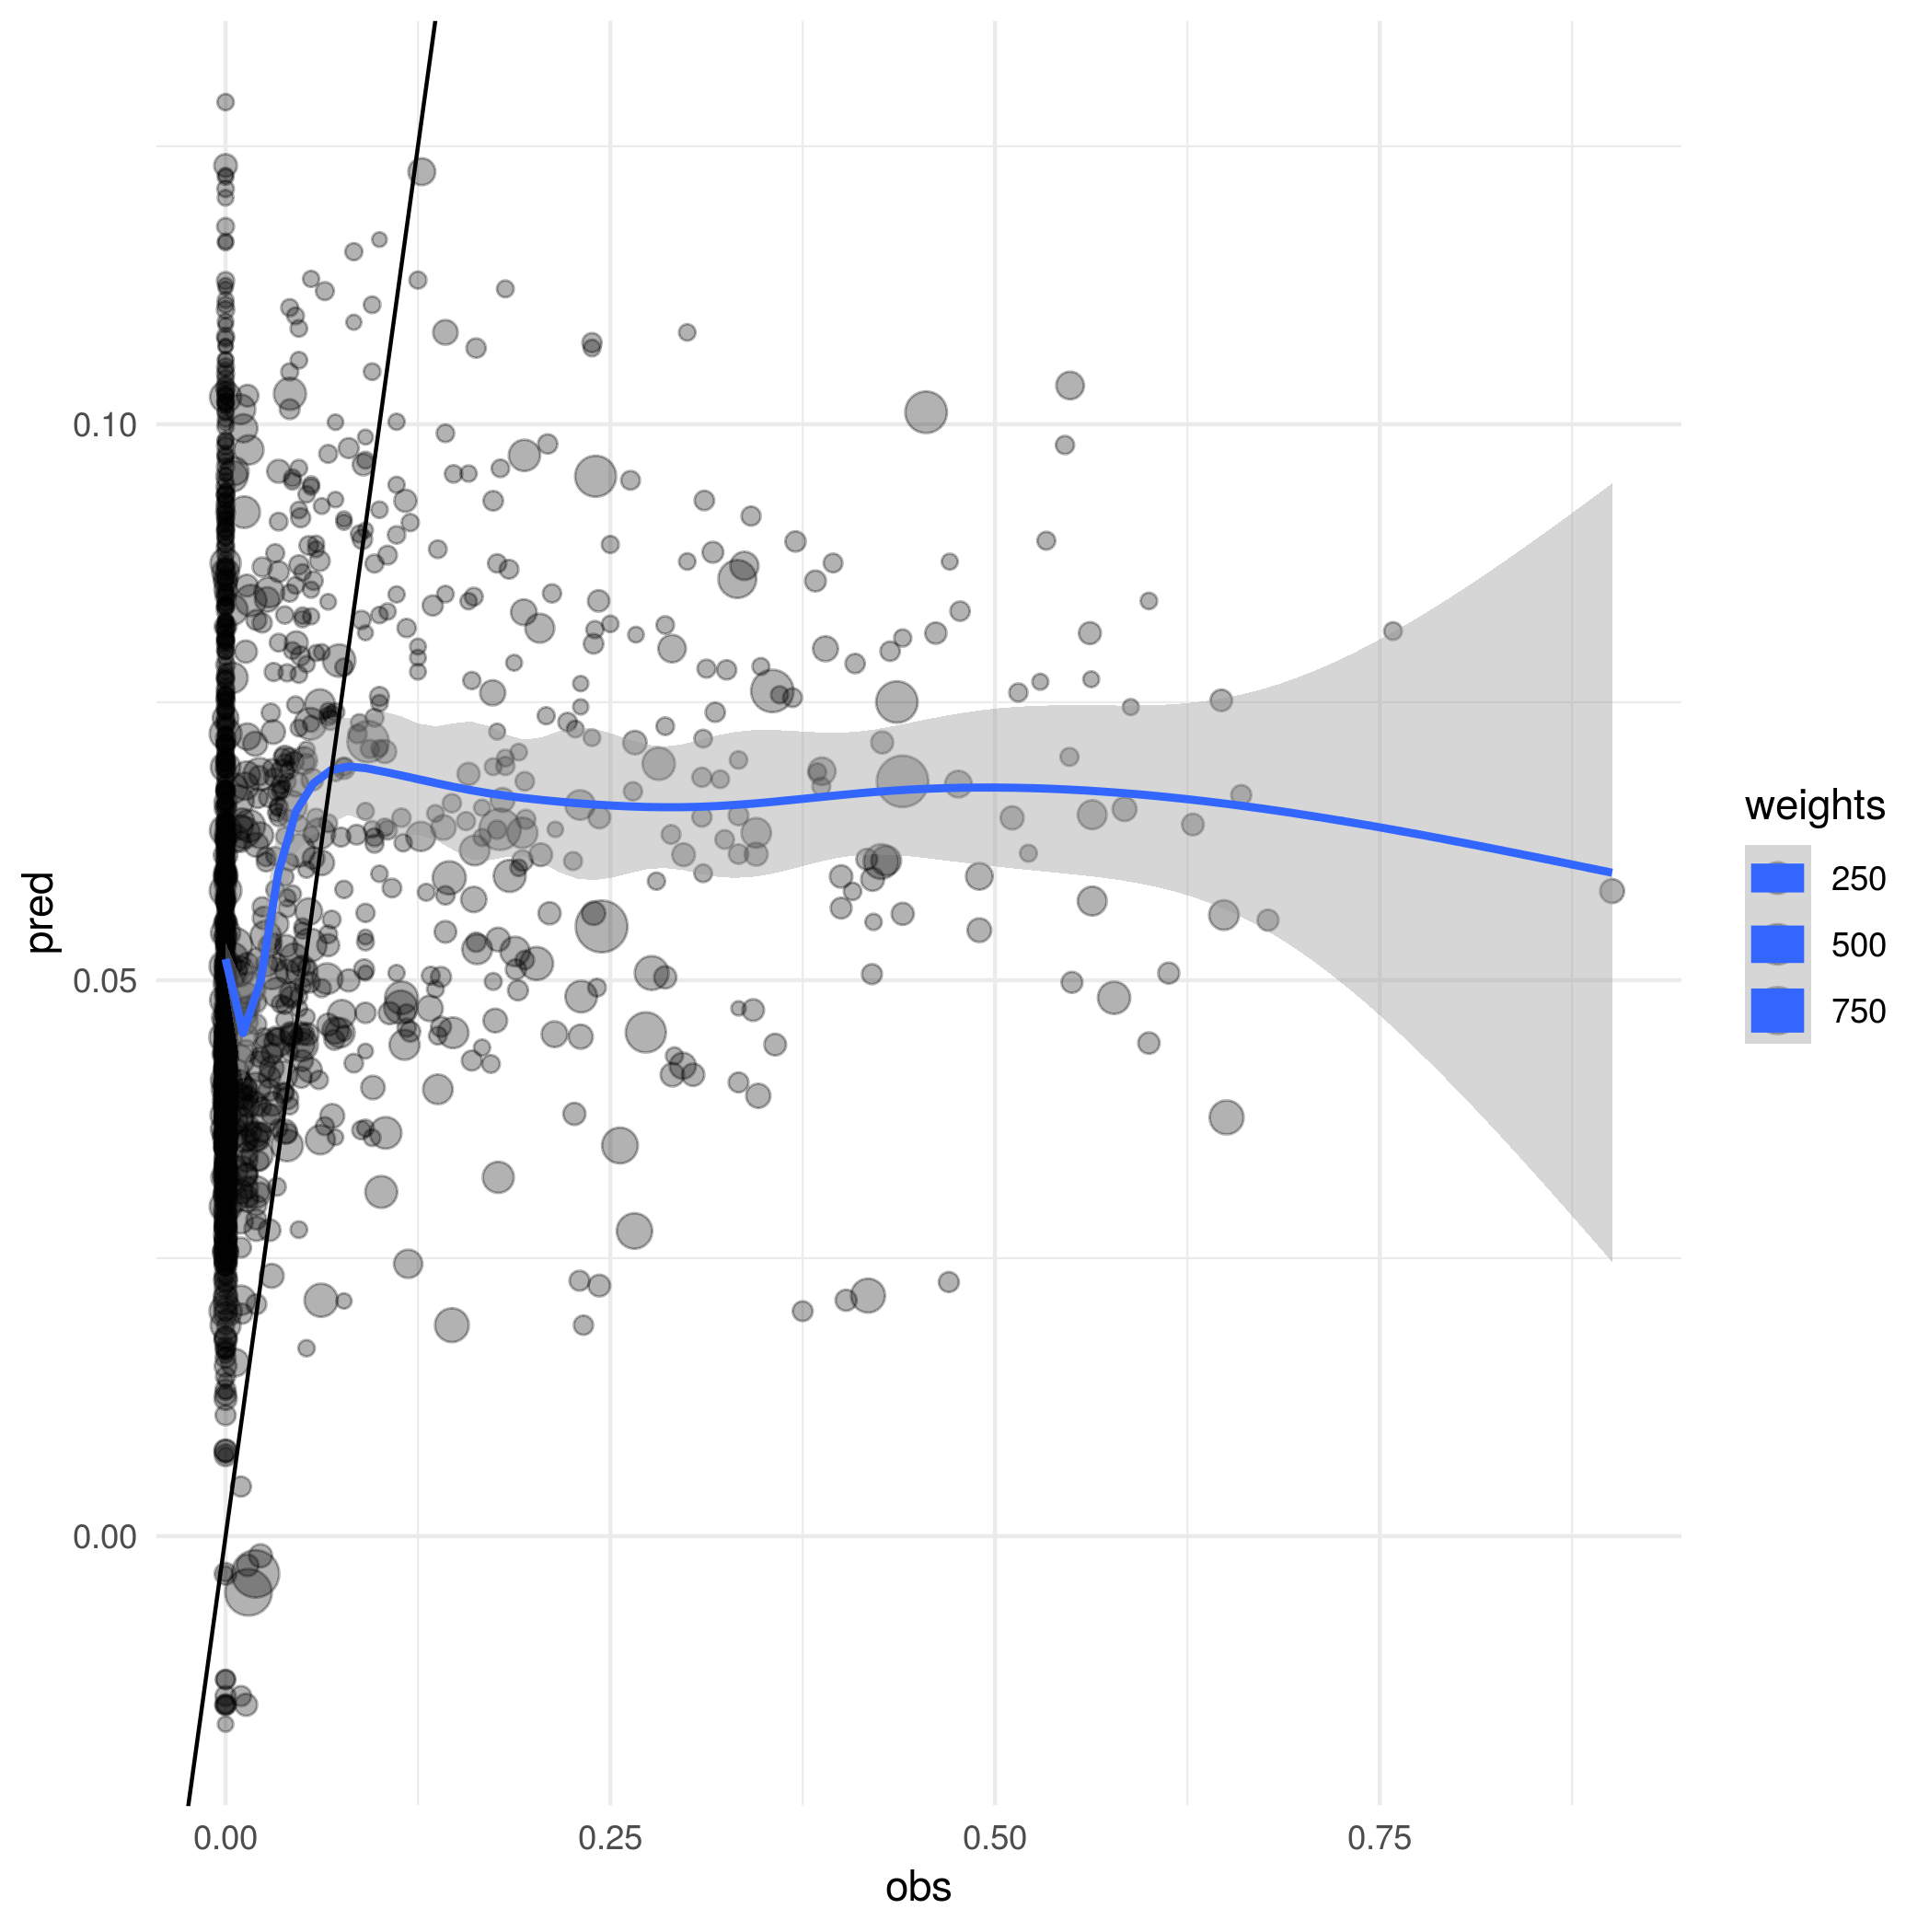
\includegraphics[width=0.6\textwidth]{figs/SI/enet_obspred_mdg.png}
\caption{
  Scatter plot of predictions and held out observed data for the elastic net trained on the Madagascar dataset.
}

\end{figure}


\begin{figure}[h!]
  \centering
  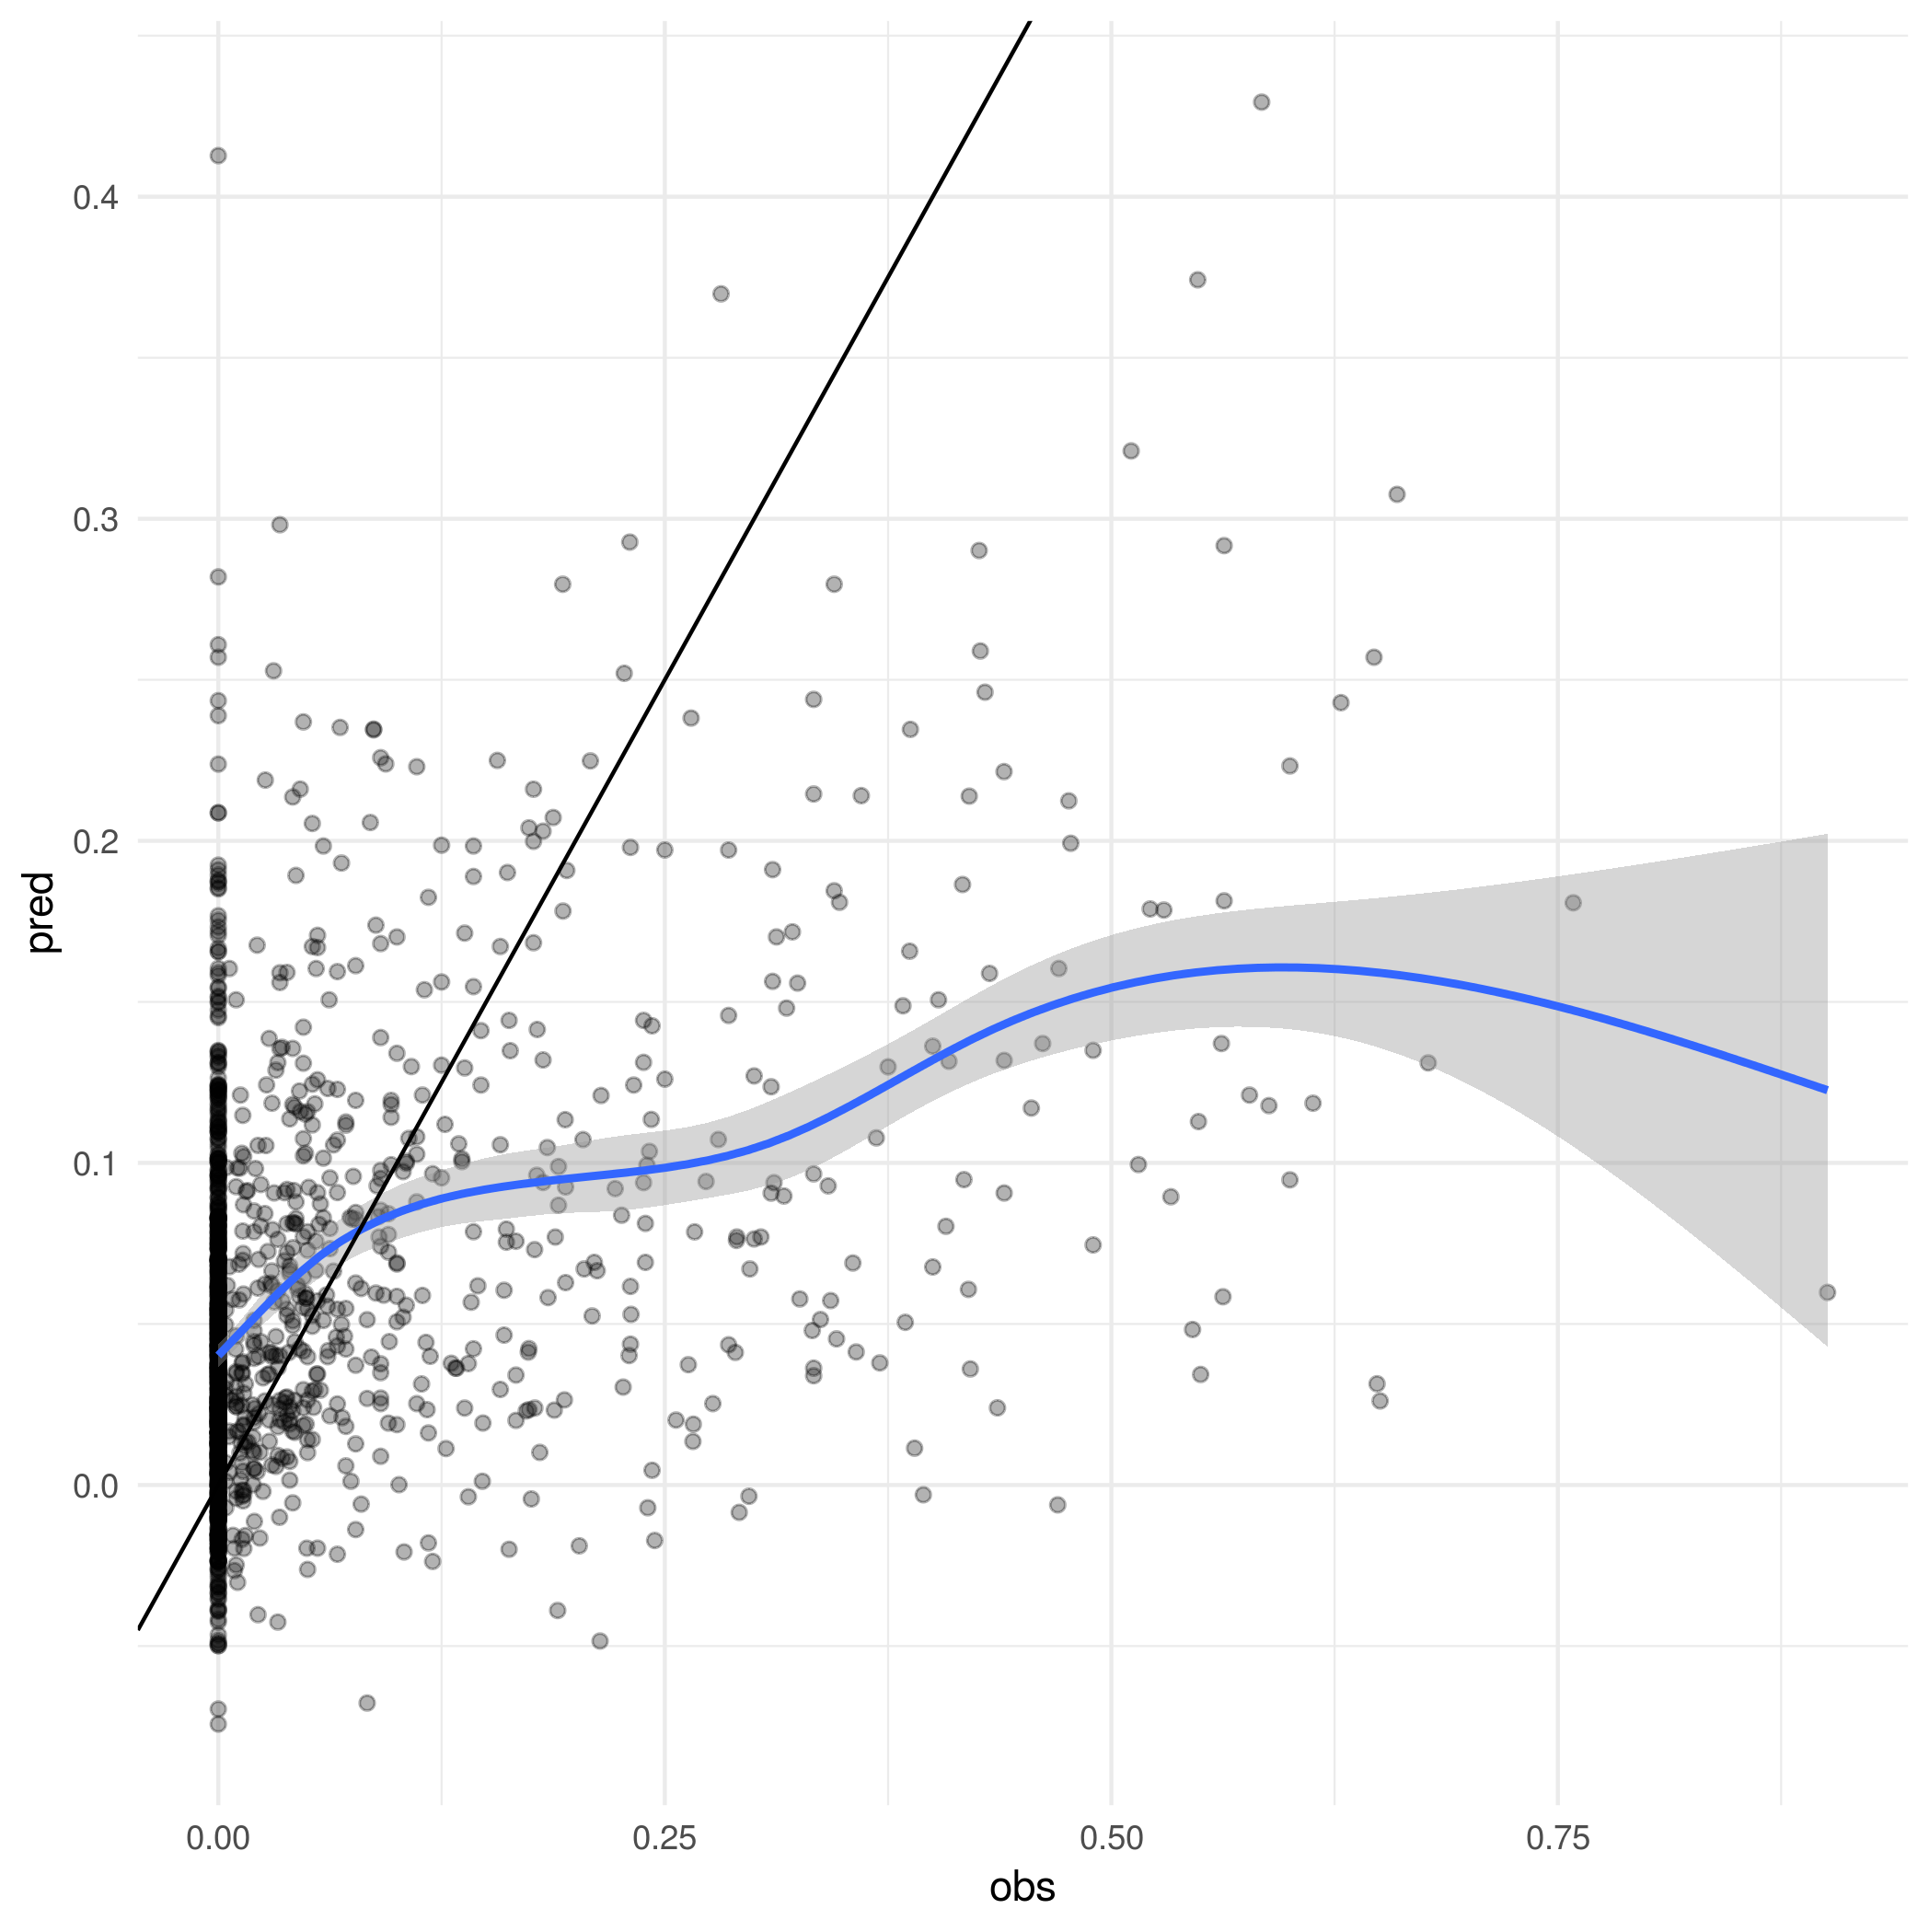
\includegraphics[width=0.6\textwidth]{figs/SI/ppr_obspred_mdg.png}
\caption{
  Scatter plot of predictions and held out observed data for the PPR trained on the Madagascar dataset.
}

\end{figure}


\begin{figure}[h!]
  \centering
  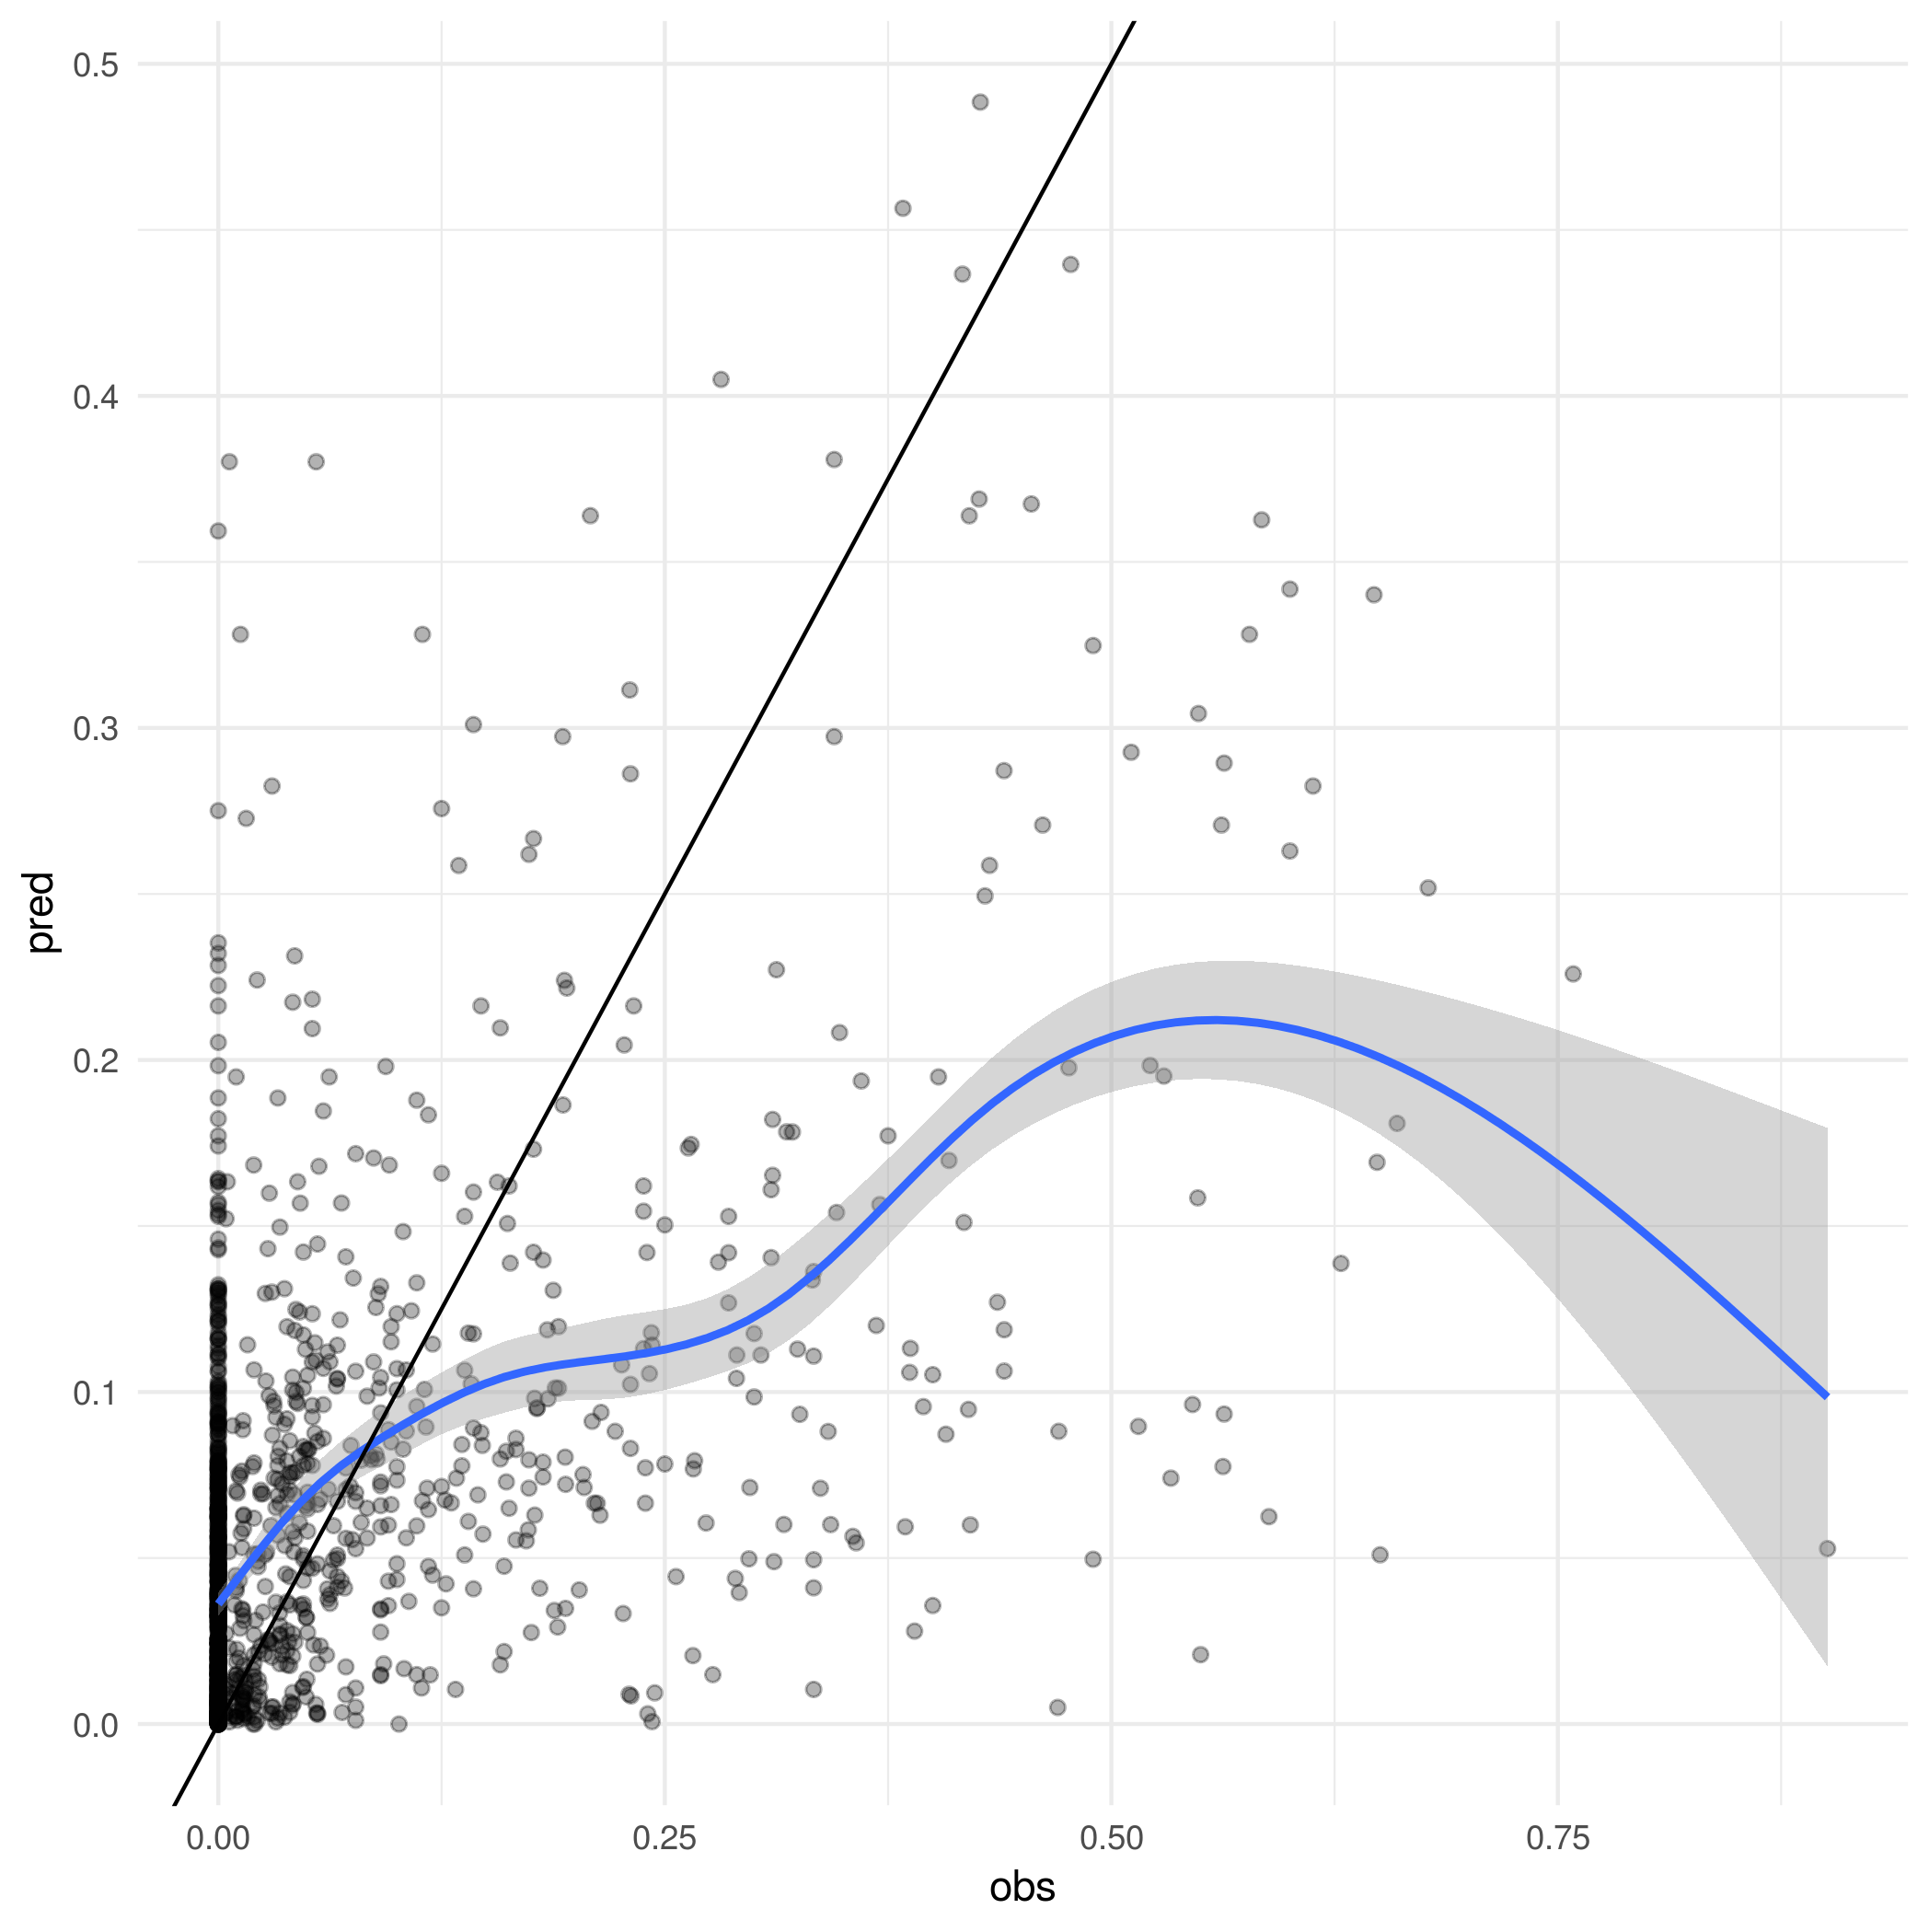
\includegraphics[width=0.6\textwidth]{figs/SI/ranger_obspred_mdg.png}
\caption{
  Scatter plot of predictions and held out observed data for the Random Forest trained on the Madagascar dataset.
}

\end{figure}


\begin{figure}[h!]
  \centering
  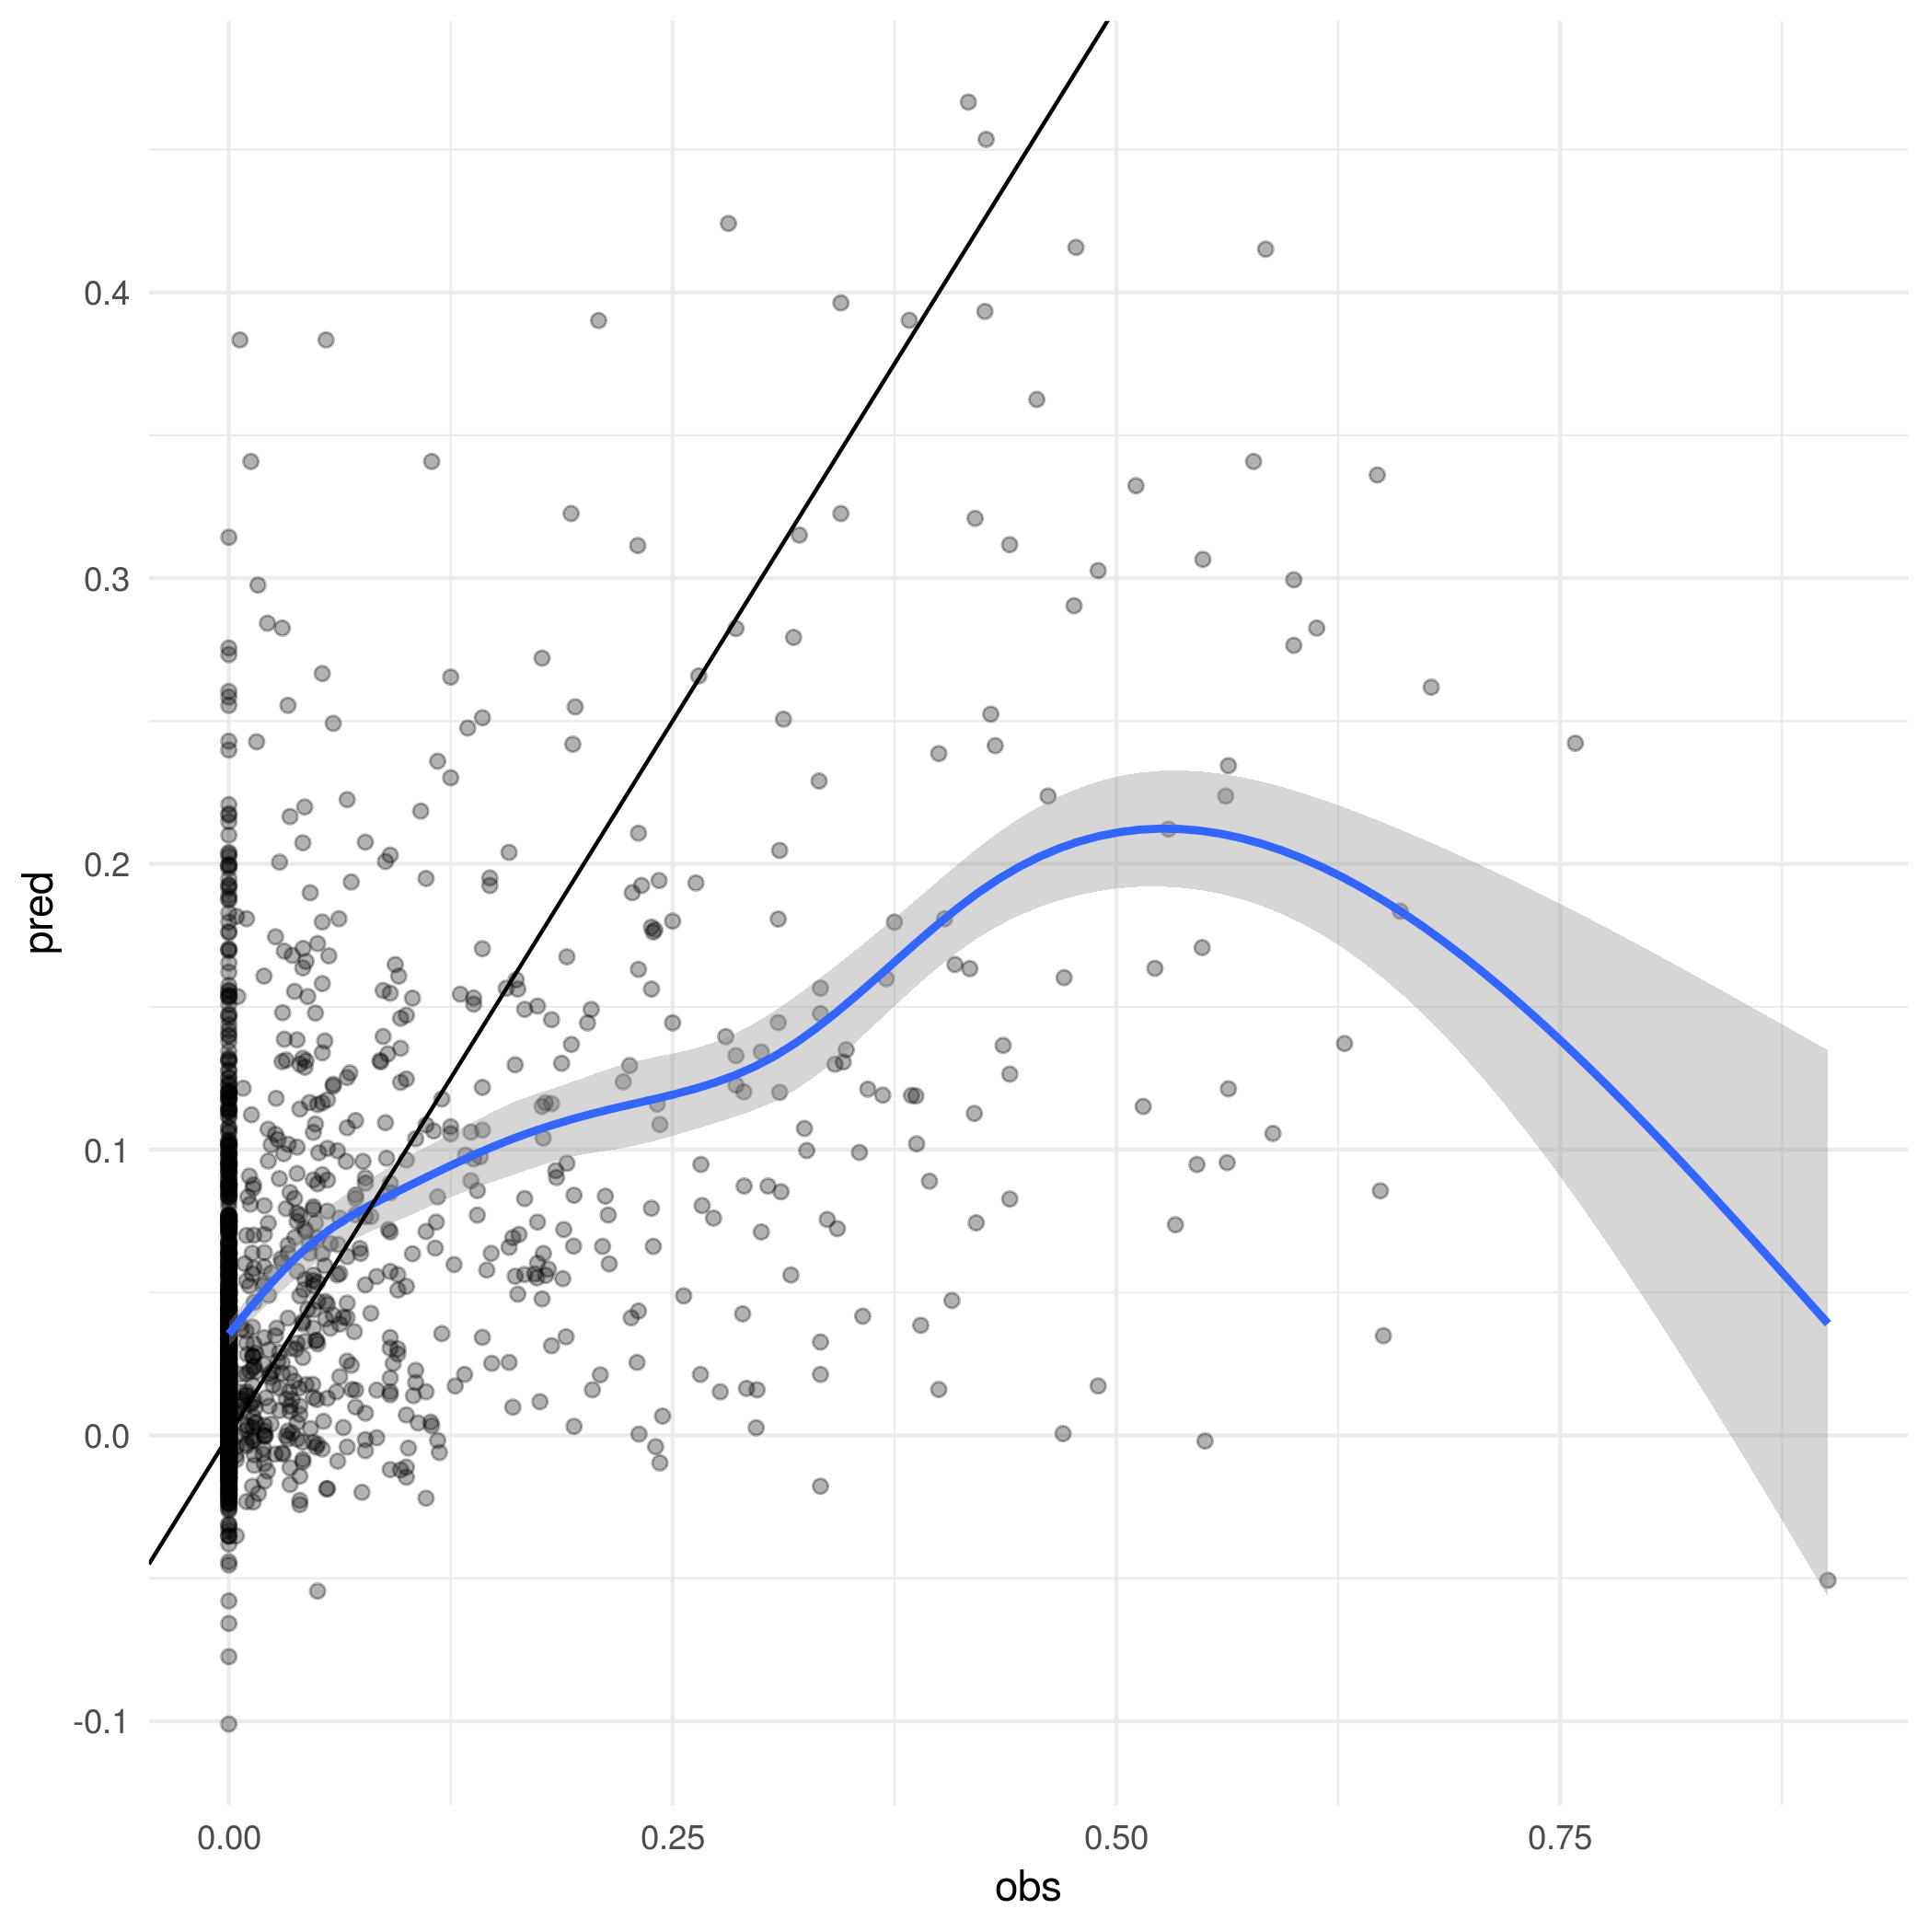
\includegraphics[width=0.6\textwidth]{figs/SI/xgboost_obspred_mdg.png}
\caption{
  Scatter plot of predictions and held out observed data for the GBM trained on the Madagascar dataset.
}

\end{figure}


\clearpage
\subsection{Hyperparameter optimisation}

As ranger and GBM were tuned with random hyperparameter search, the plots become difficult and are not included.


\begin{figure}[h!]
  \centering
  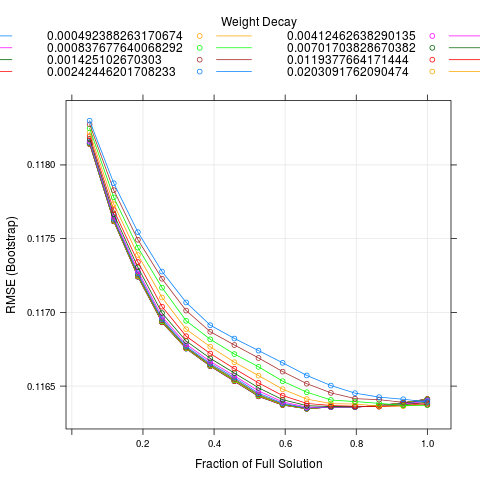
\includegraphics[width=0.6\textwidth]{figs/SI/enetopt_mdg.png}
\caption{
  Optimisation for elastic net hyperparameters trained on the Madagascar dataset.
}
\end{figure}



\begin{figure}[h!]
  \centering
  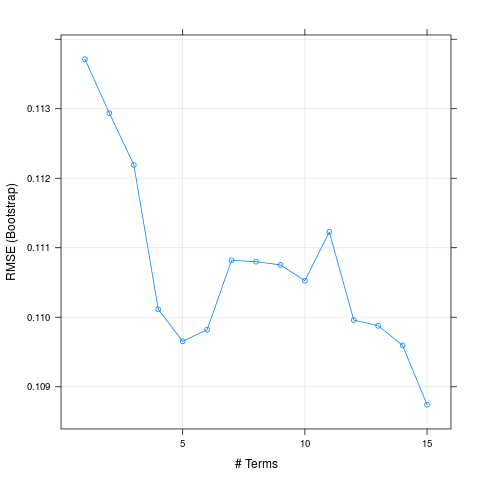
\includegraphics[width=0.6\textwidth]{figs/SI/ppropt_mdg.png}
\caption{
  Optimisation for PPR hyperparameters trained on the Madagascar dataset.
}

\end{figure}








\clearpage
%%%%%%%%%%%%%%%%%%%%%%%%%%%%%%%%%%%%%%%%%%%%%%%%%%%%%%%%%%%%%%%%%%%%%%%
\section{Senegal dataset Machine Learning}
%%%%%%%%%%%%%%%%%%%%%%%%%%%%%%%%%%%%%%%%%%%%%%%%%%%%%%%%%%%%%%%%%%%%%%%






\subsection{Predictions}

\begin{figure}[h!]
  \centering
  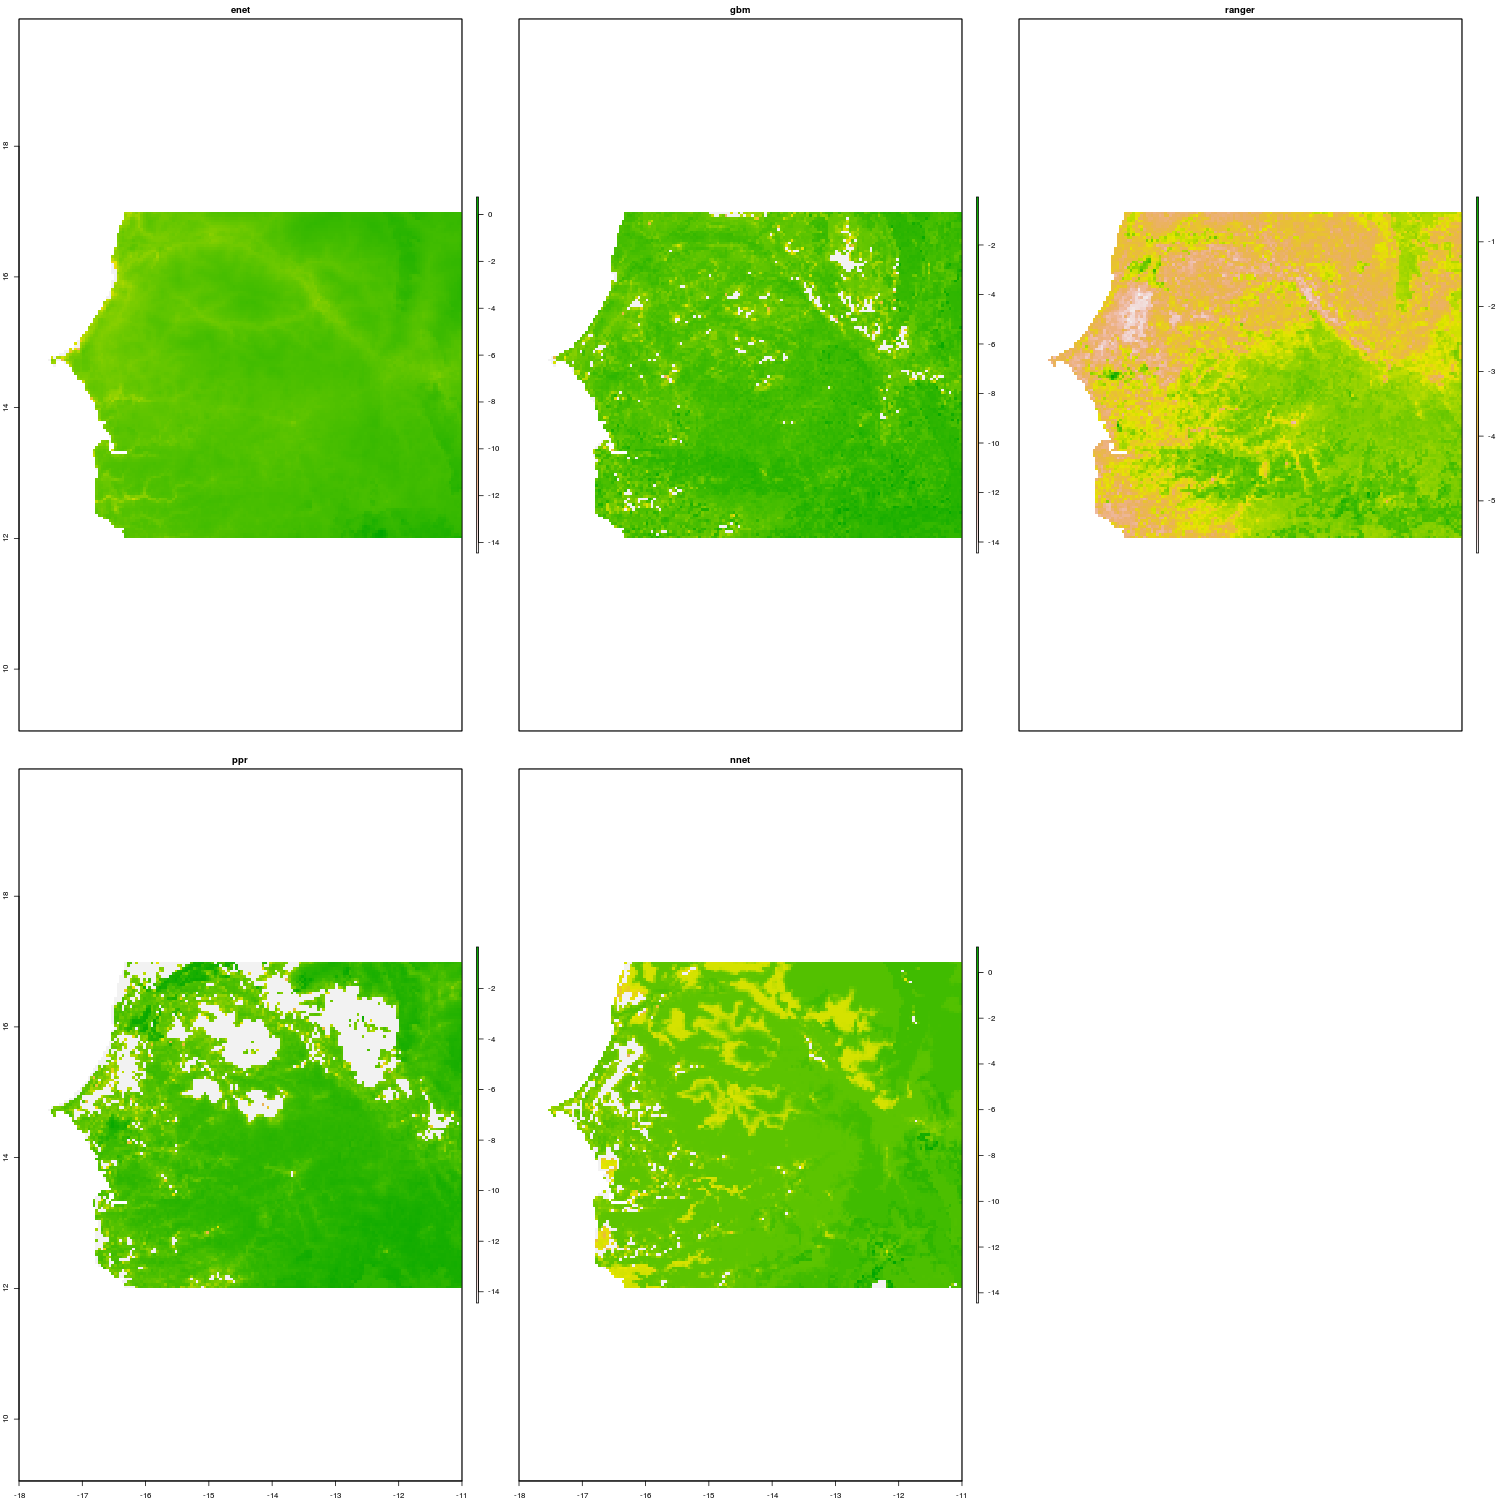
\includegraphics[width=1\textwidth]{figs/SI/sen_all_ml.png}
\caption{
  Predictions from machine learning models trained on Senegal prevalence data.
}

\end{figure}


\begin{figure}[h!]
  \centering
  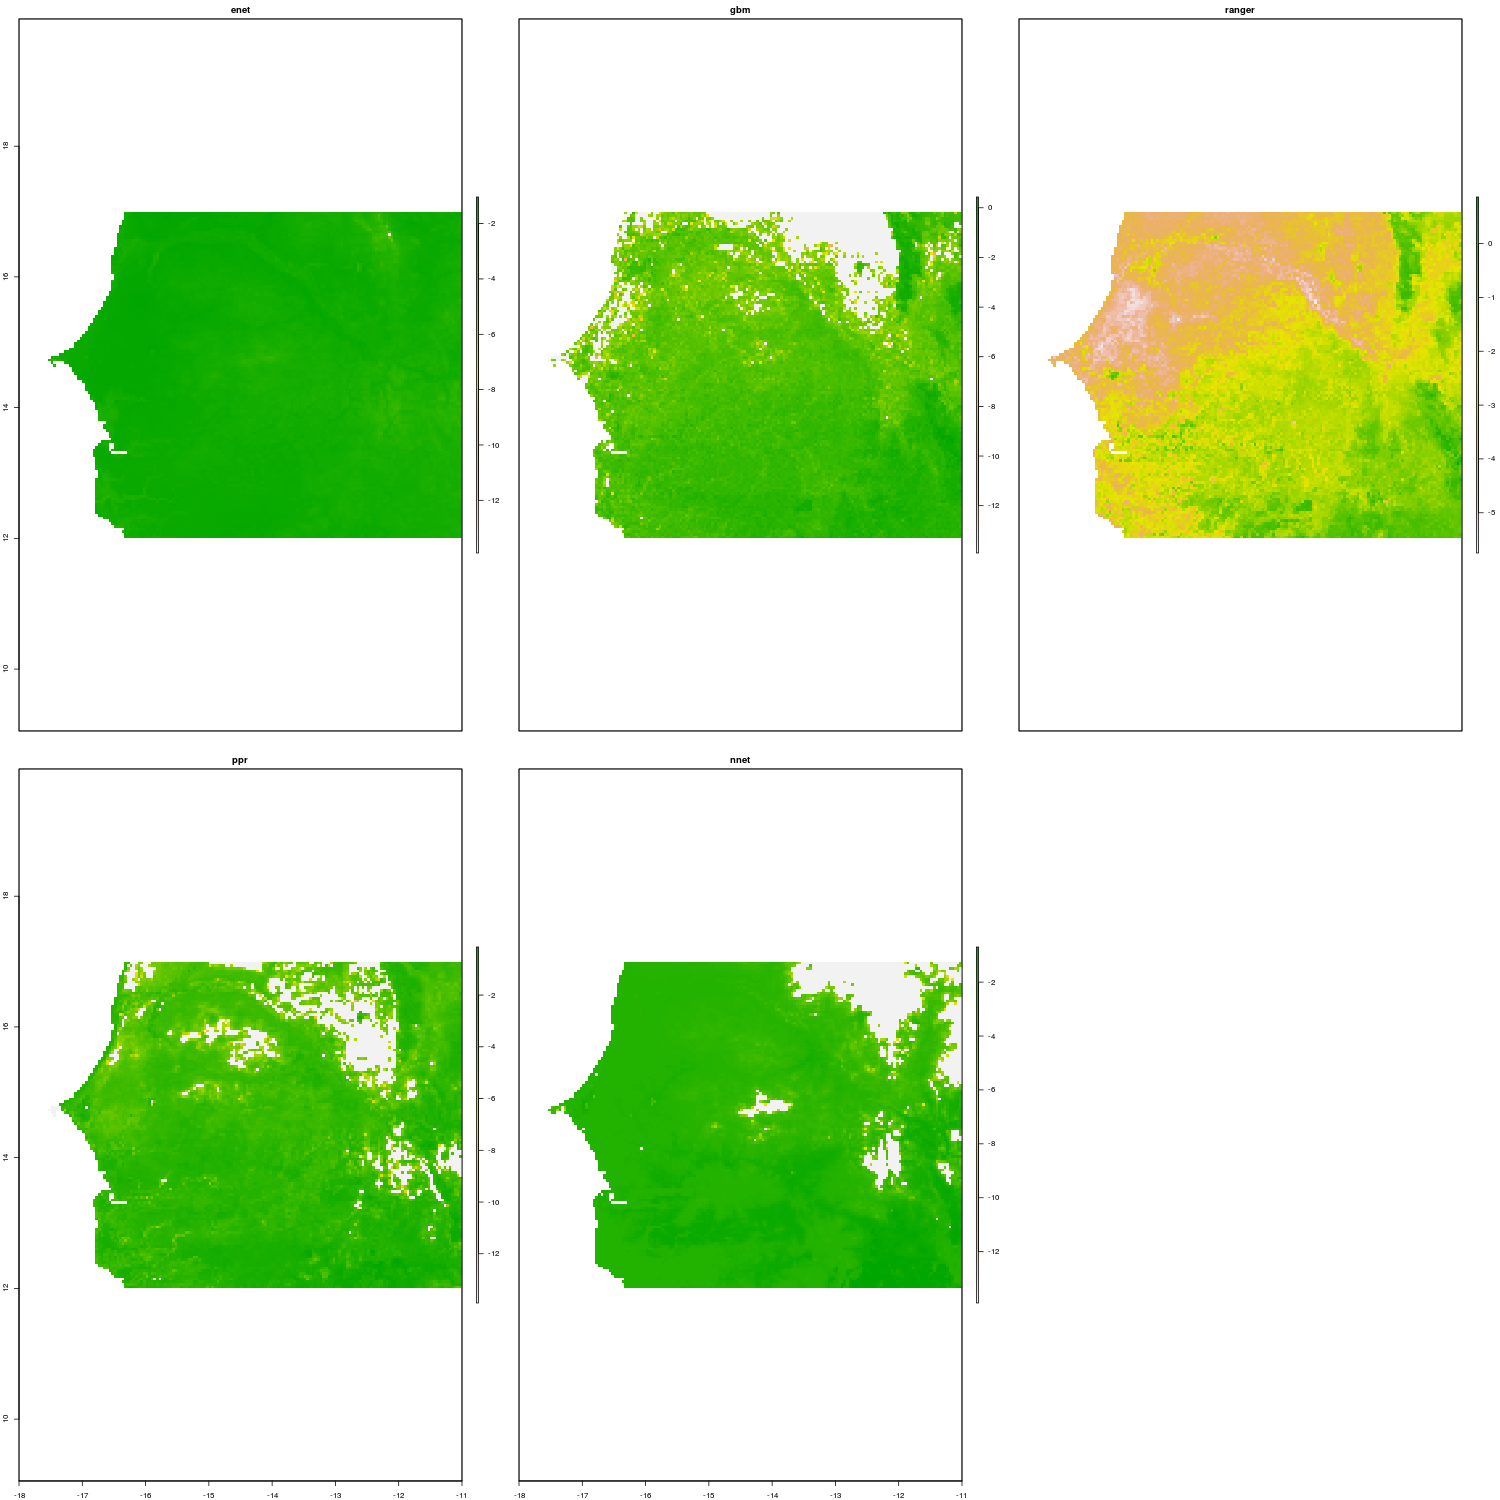
\includegraphics[width=1\textwidth]{figs/SI/sen_all_globalml.png}
\caption{
  Predictions from machine learning models trained on Senegal prevalence data.
}

\end{figure}



\clearpage
\subsection{Out-of-sample scatter plots}


\begin{figure}[h!]
  \centering
  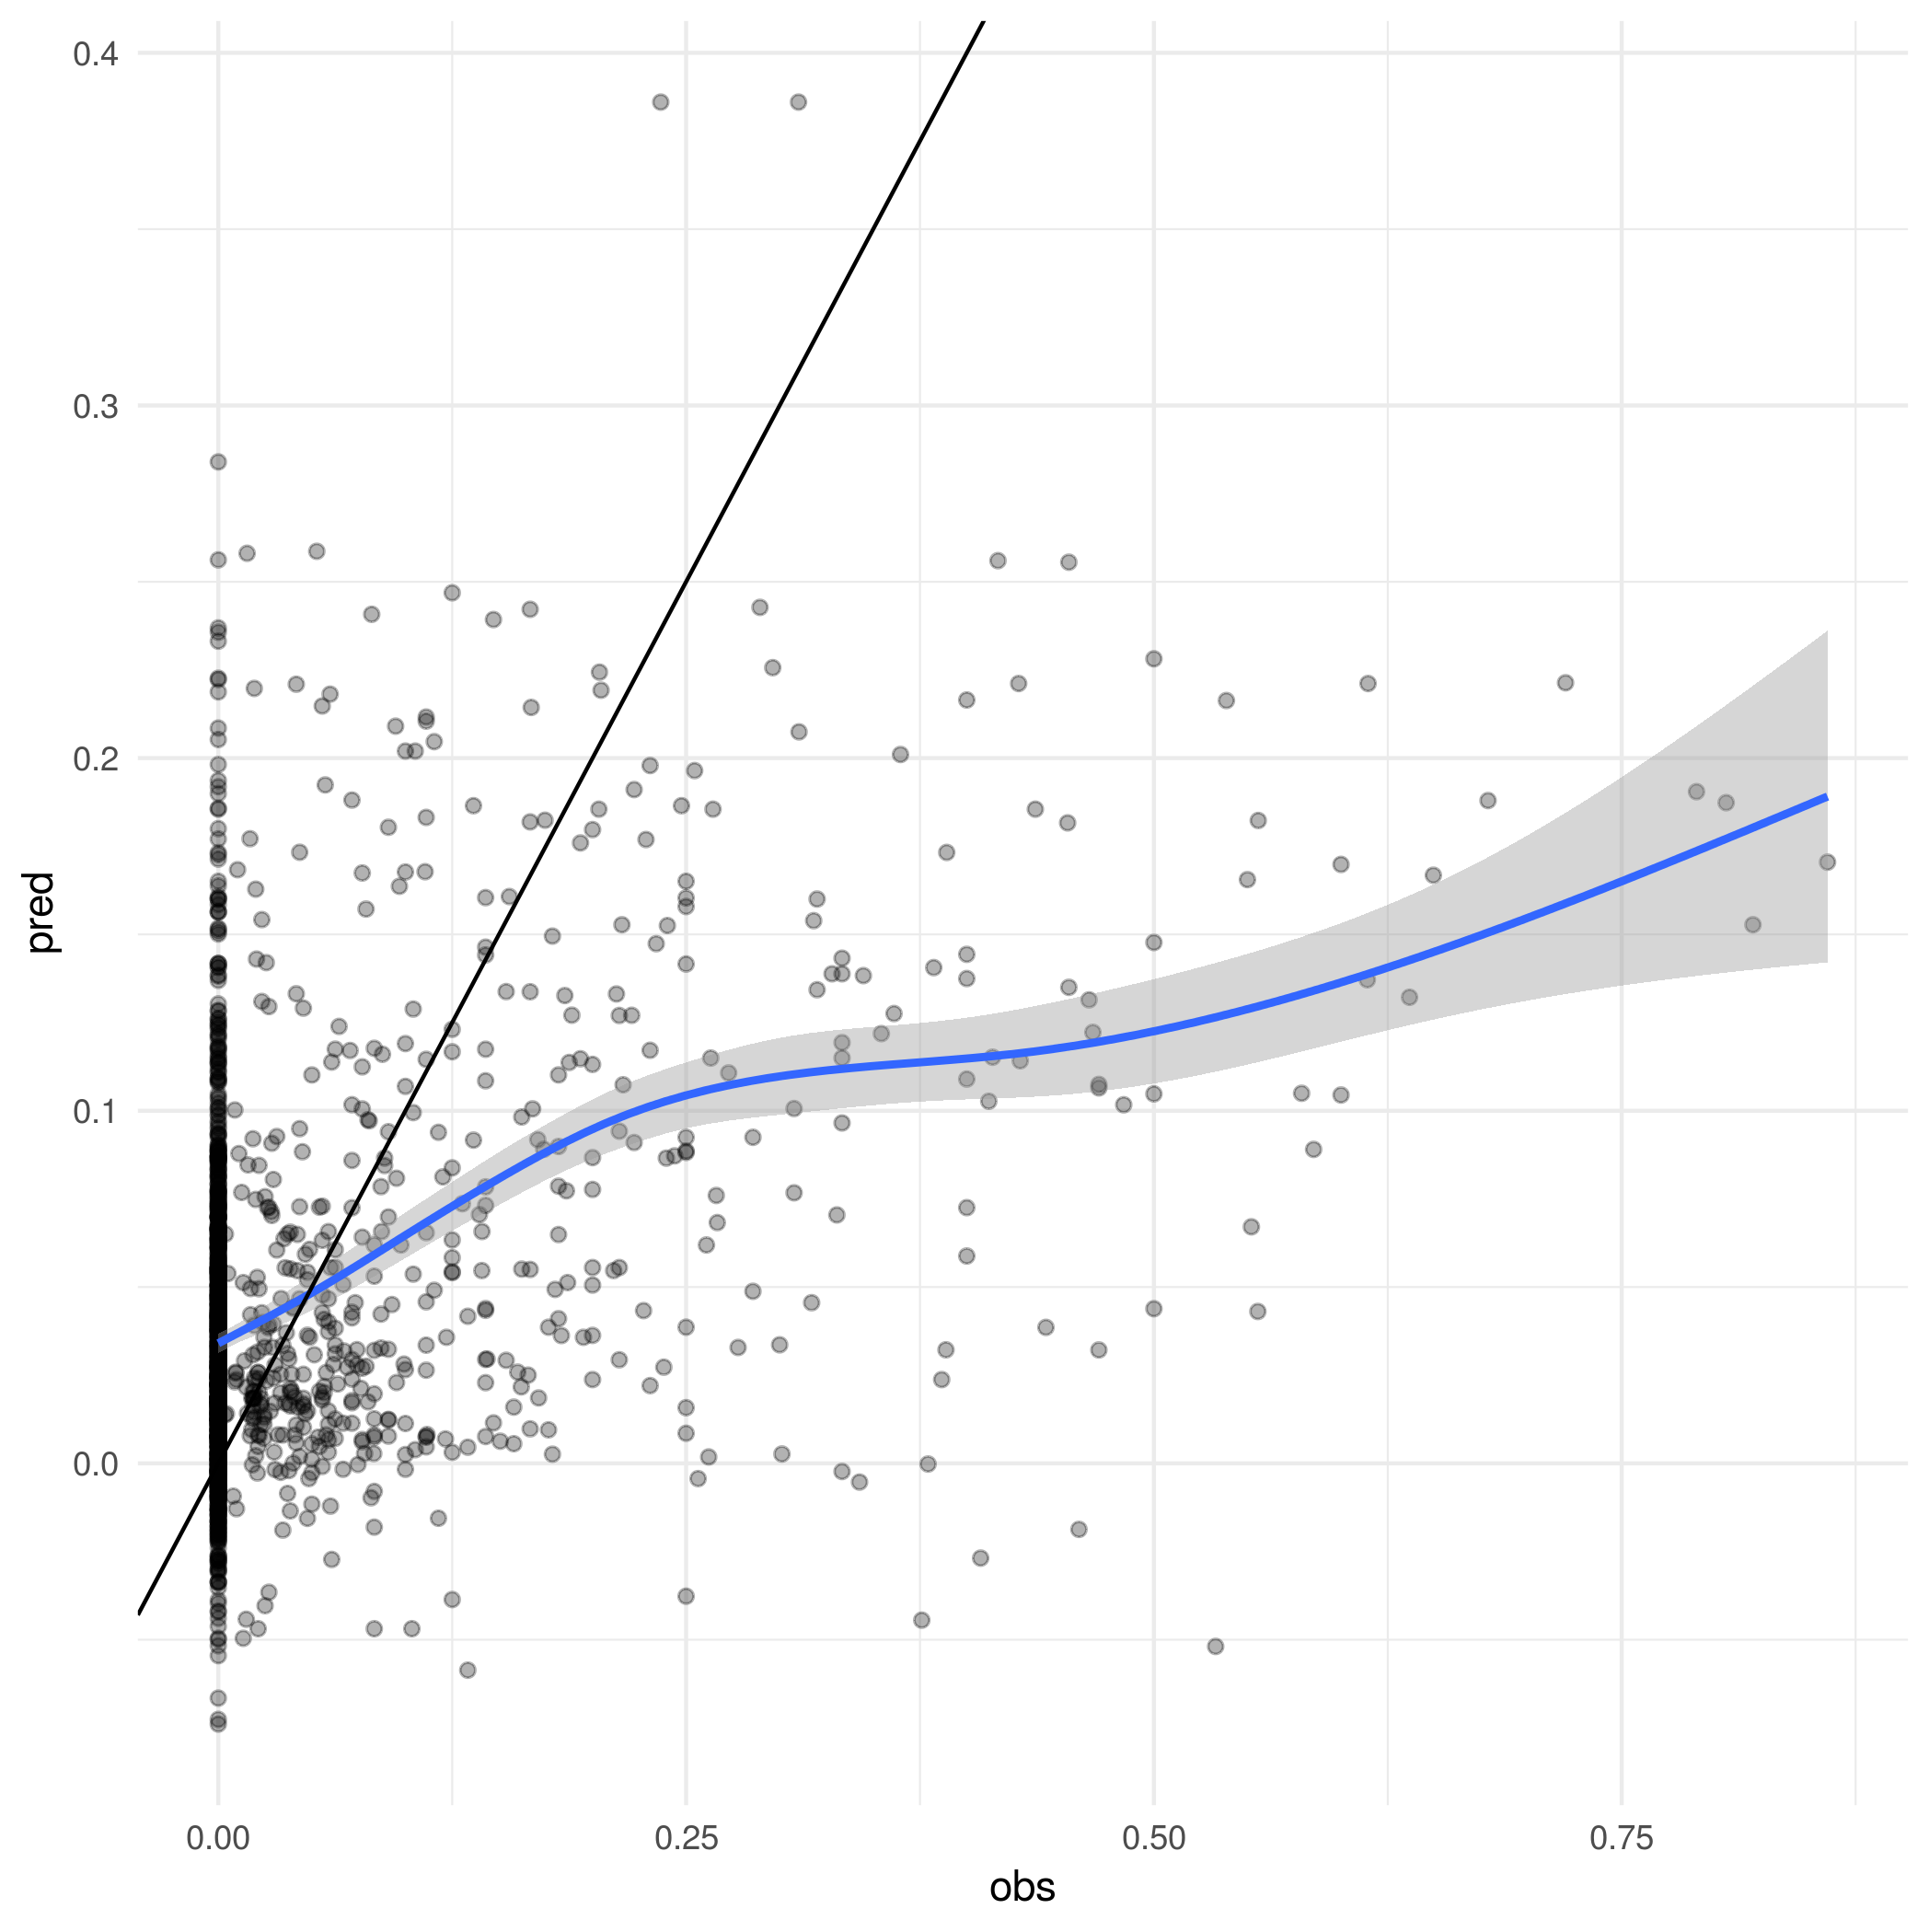
\includegraphics[width=0.6\textwidth]{figs/SI/nnet_obspred_sen.png}
\caption{
  Scatter plot of predictions and held out observed data for the neural network trained on the Senegal dataset.
}

\end{figure}



\begin{figure}[h!]
  \centering
  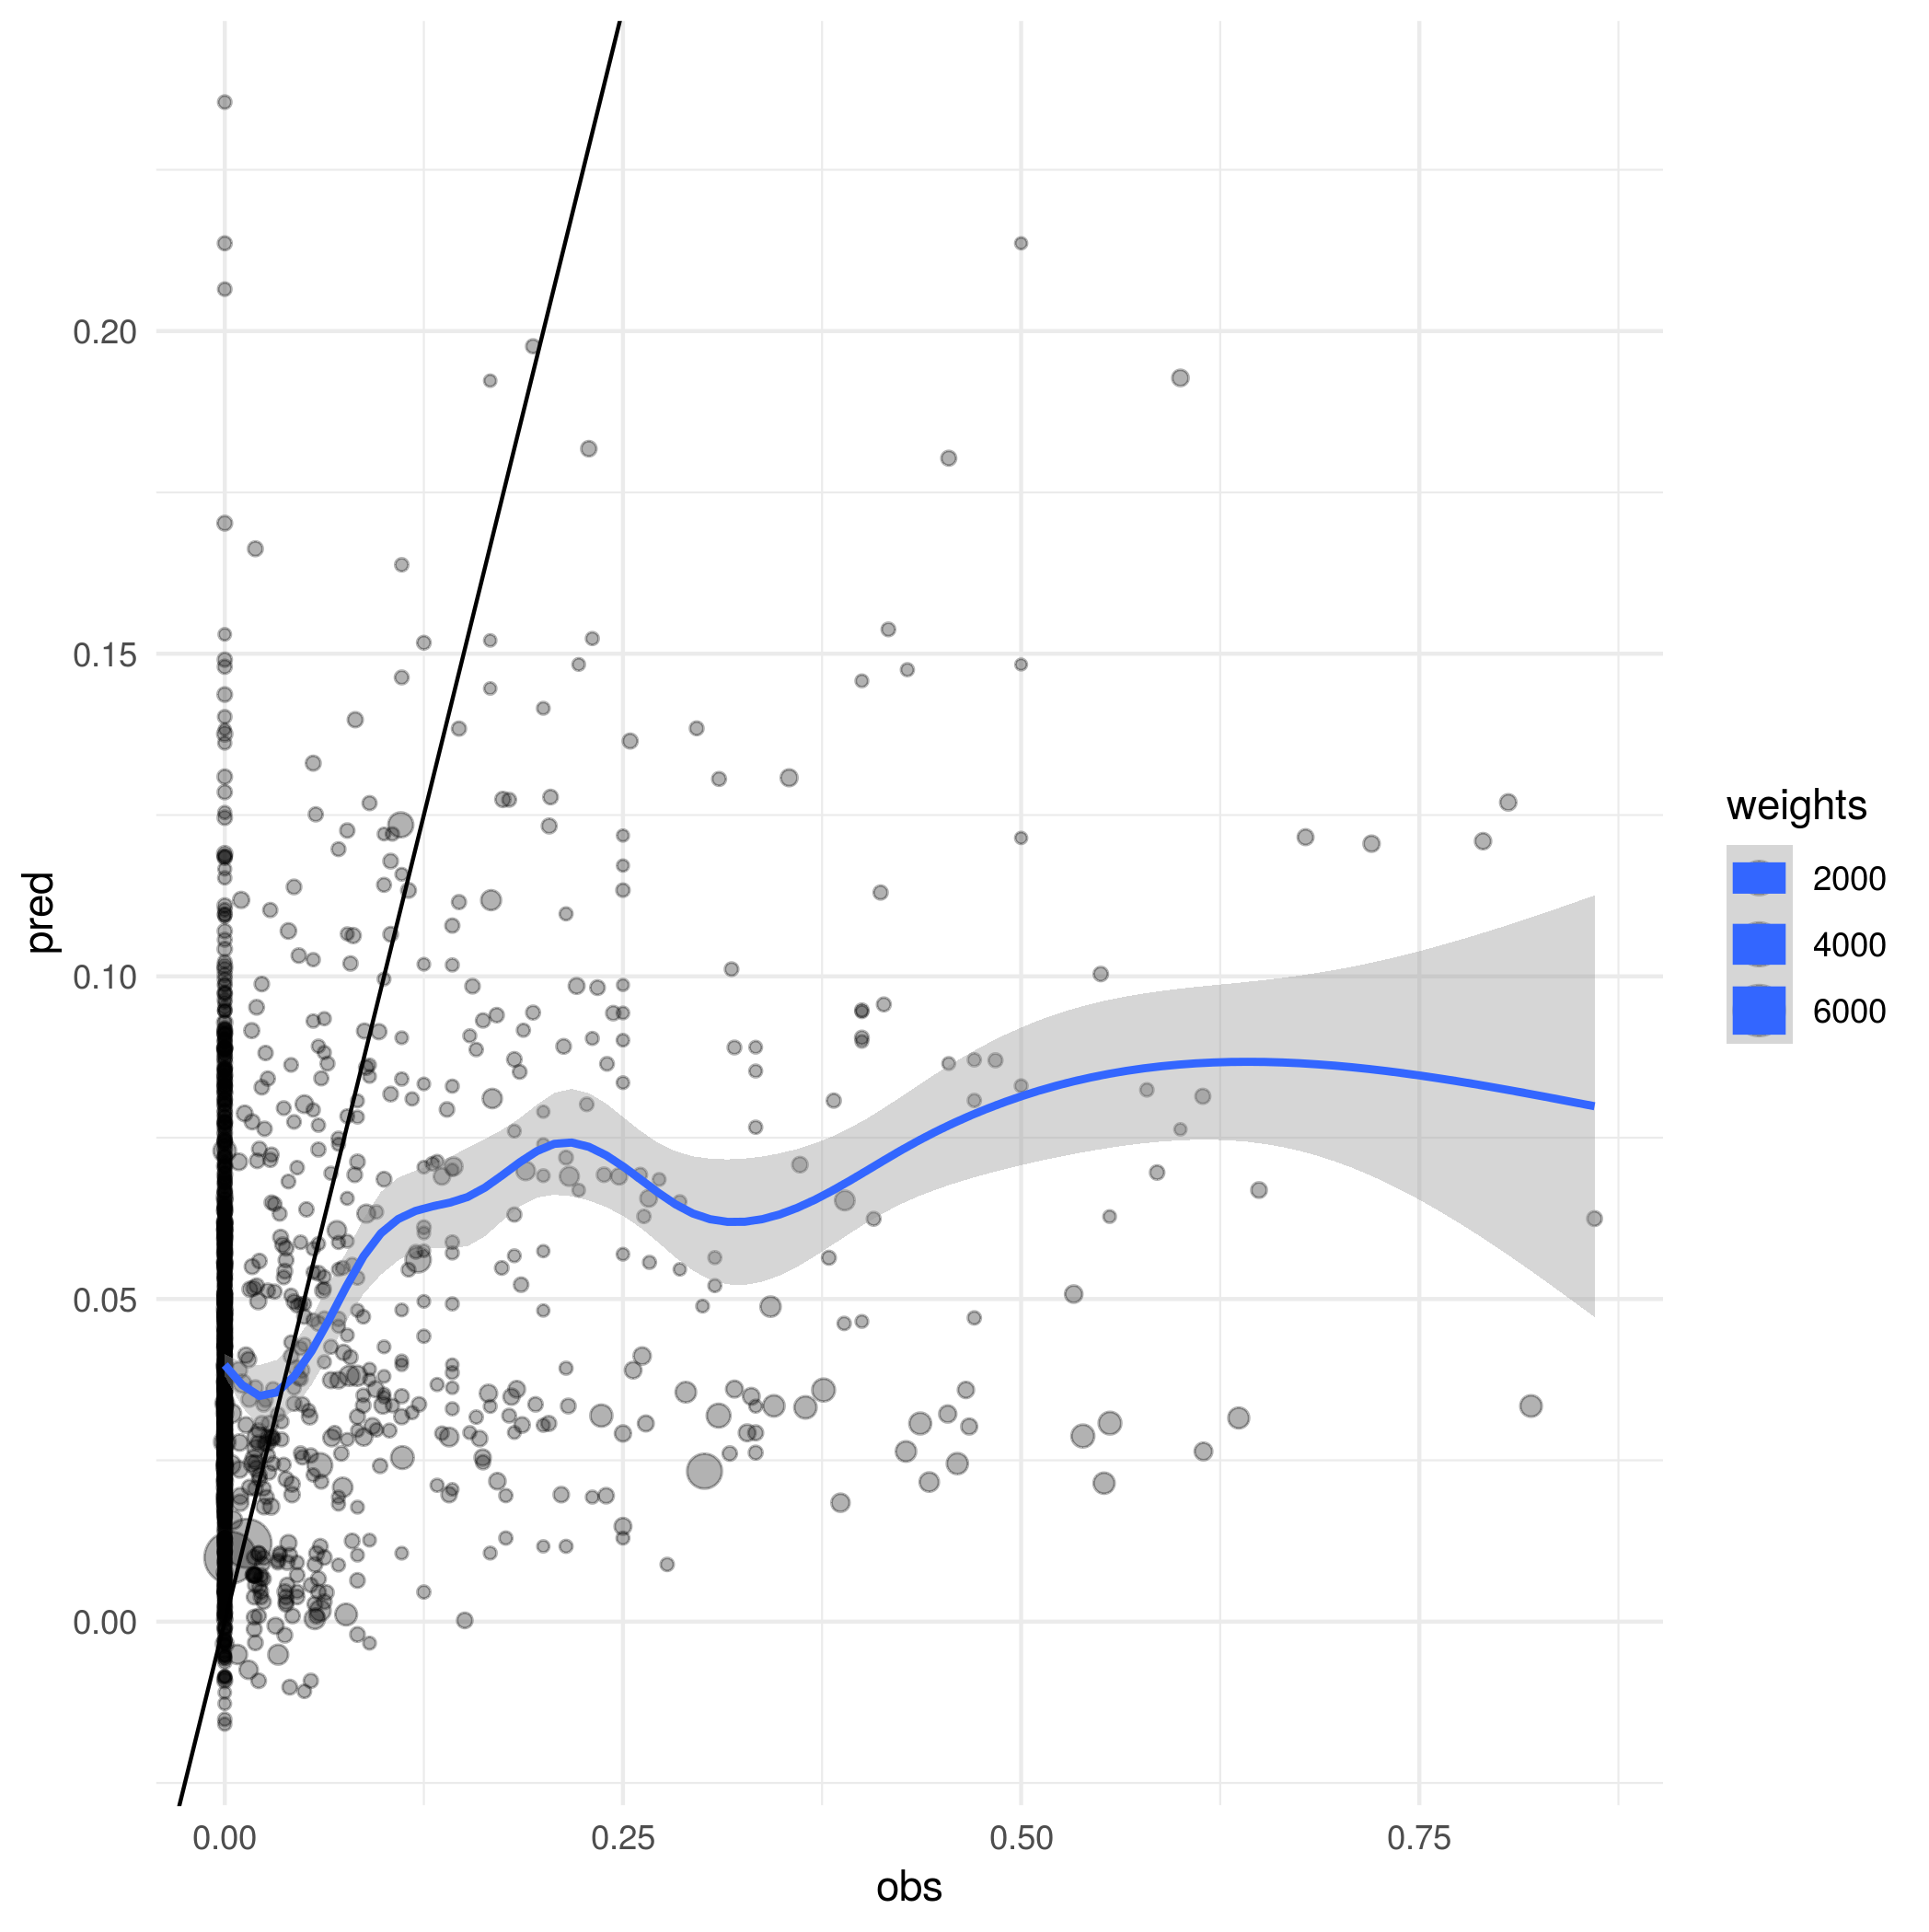
\includegraphics[width=0.6\textwidth]{figs/SI/enet_obspred_sen.png}
\caption{
  Scatter plot of predictions and held out observed data for the elastic net trained on the Senegal dataset.
}

\end{figure}


\begin{figure}[h!]
  \centering
  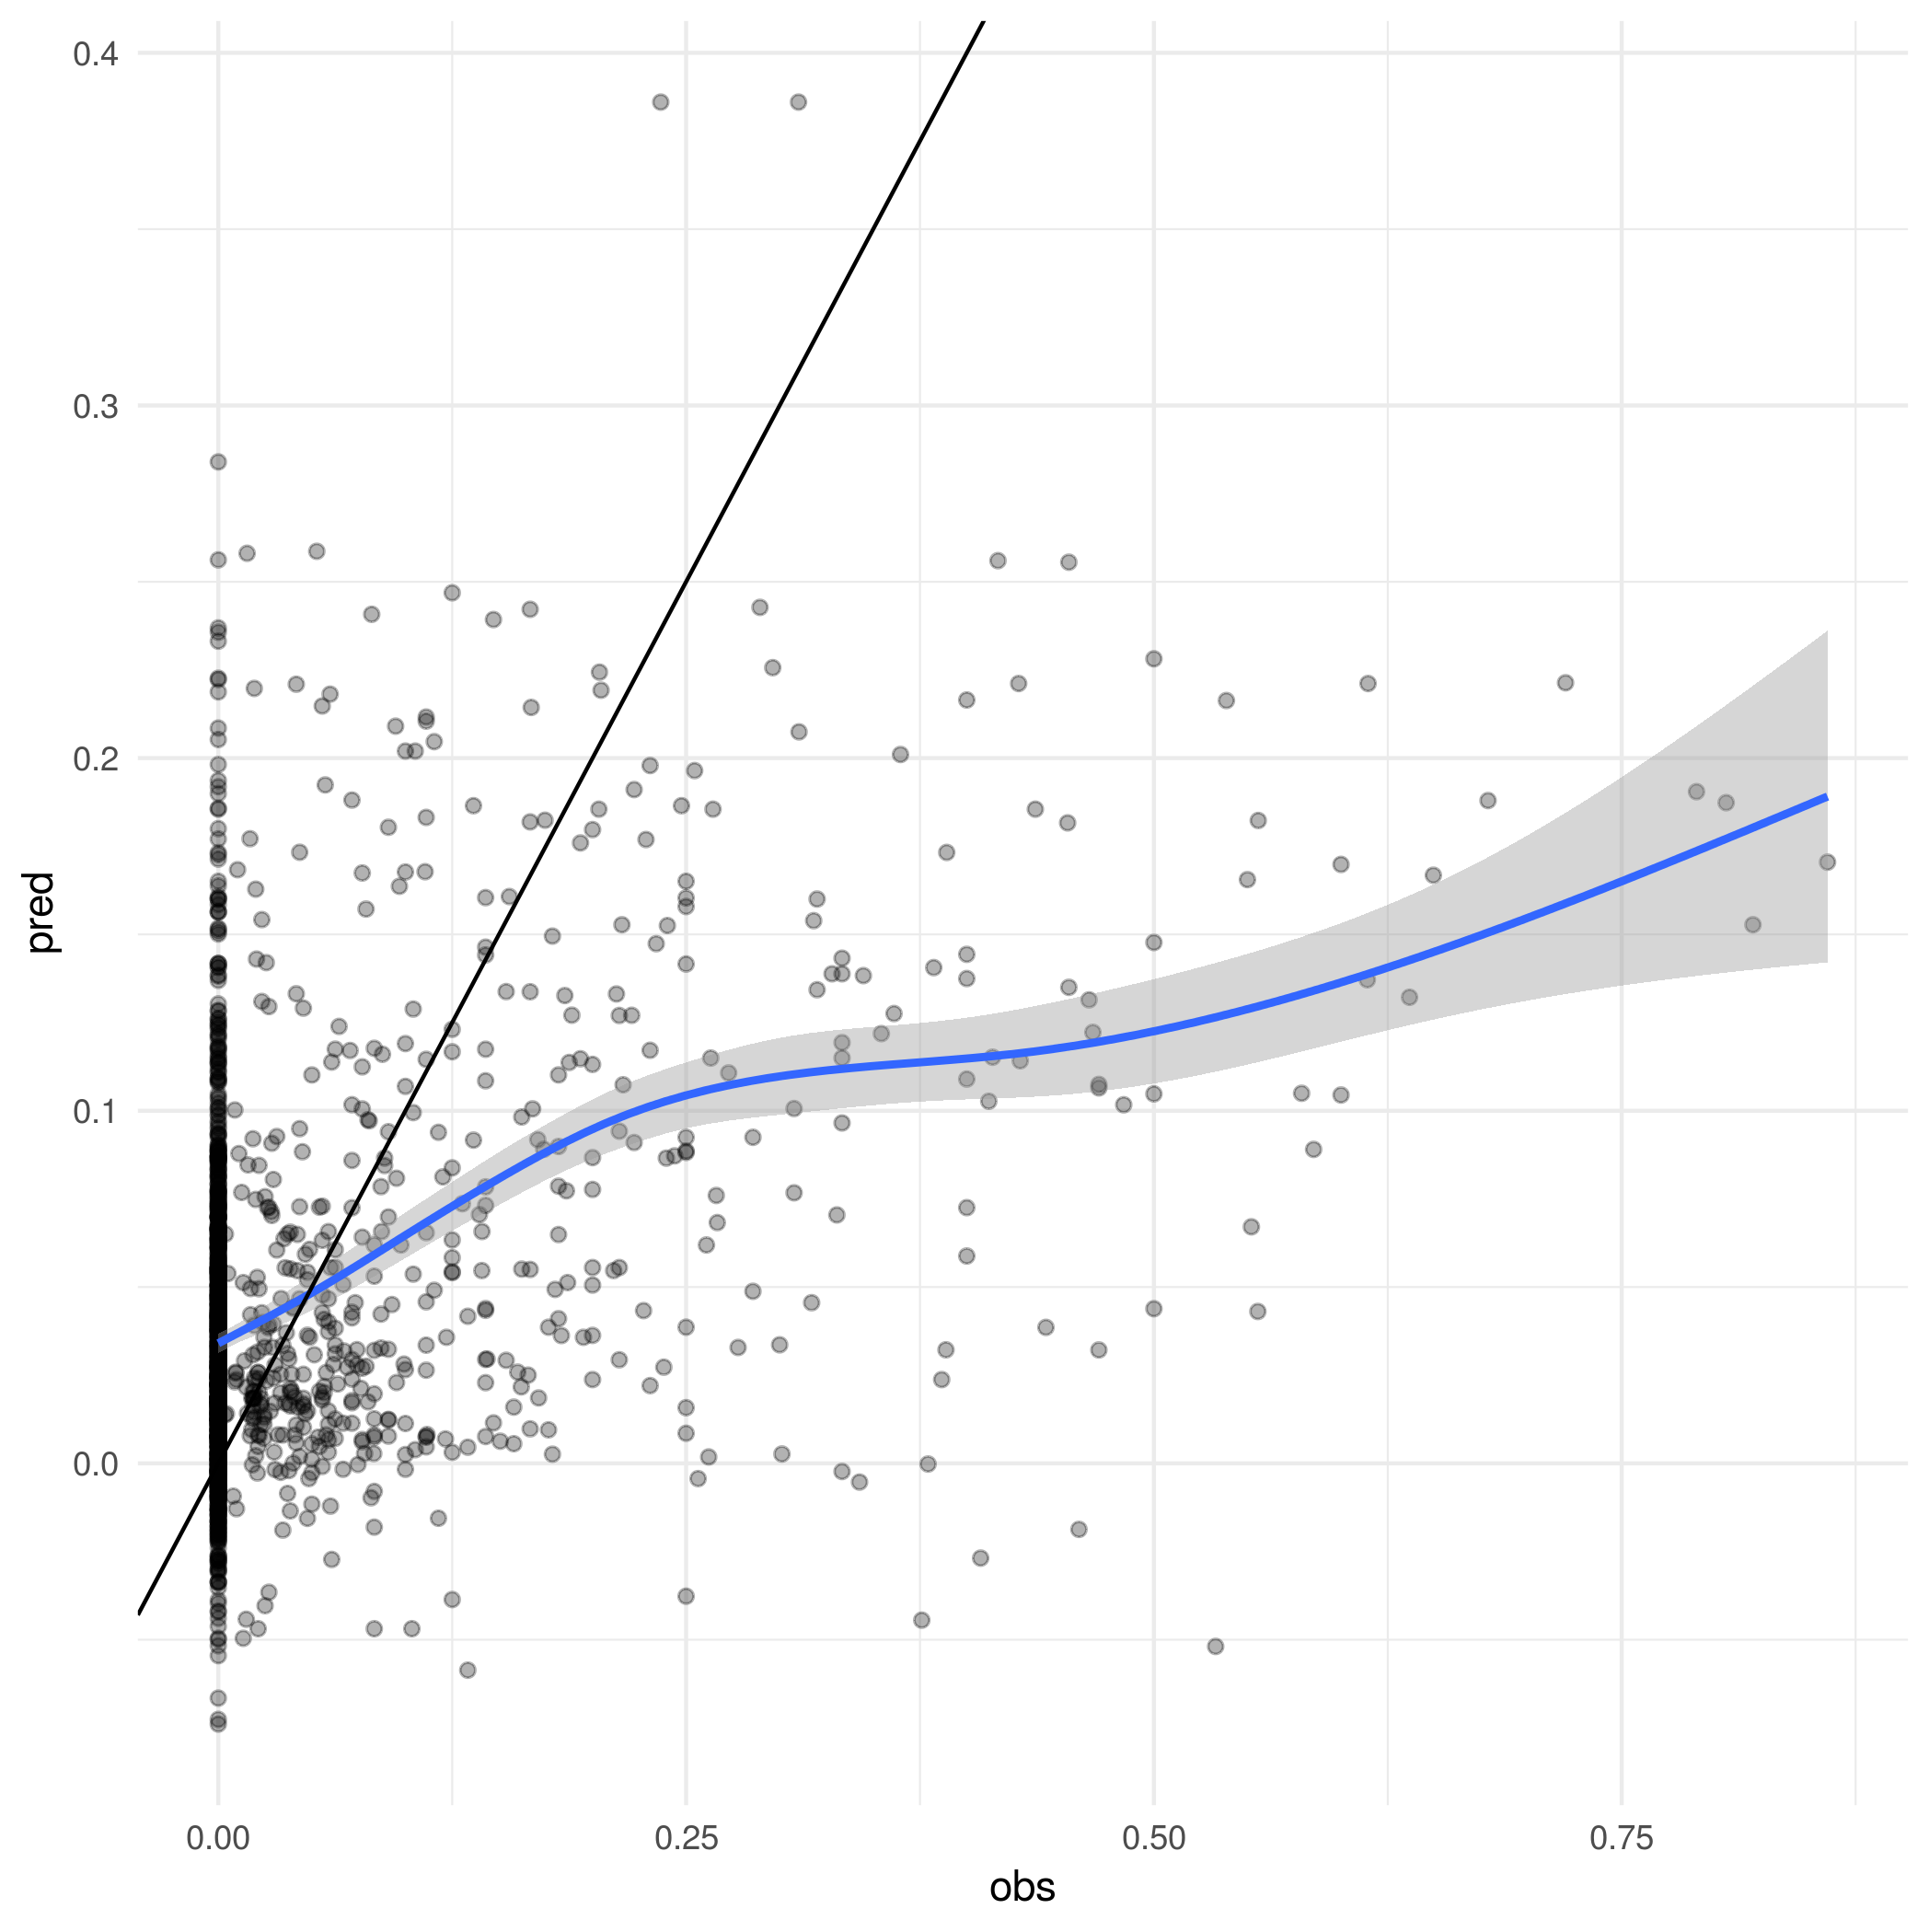
\includegraphics[width=0.6\textwidth]{figs/SI/ppr_obspred_sen.png}
\caption{
  Scatter plot of predictions and held out observed data for the PPR trained on the Senegal dataset.
}

\end{figure}


\begin{figure}[h!]
  \centering
  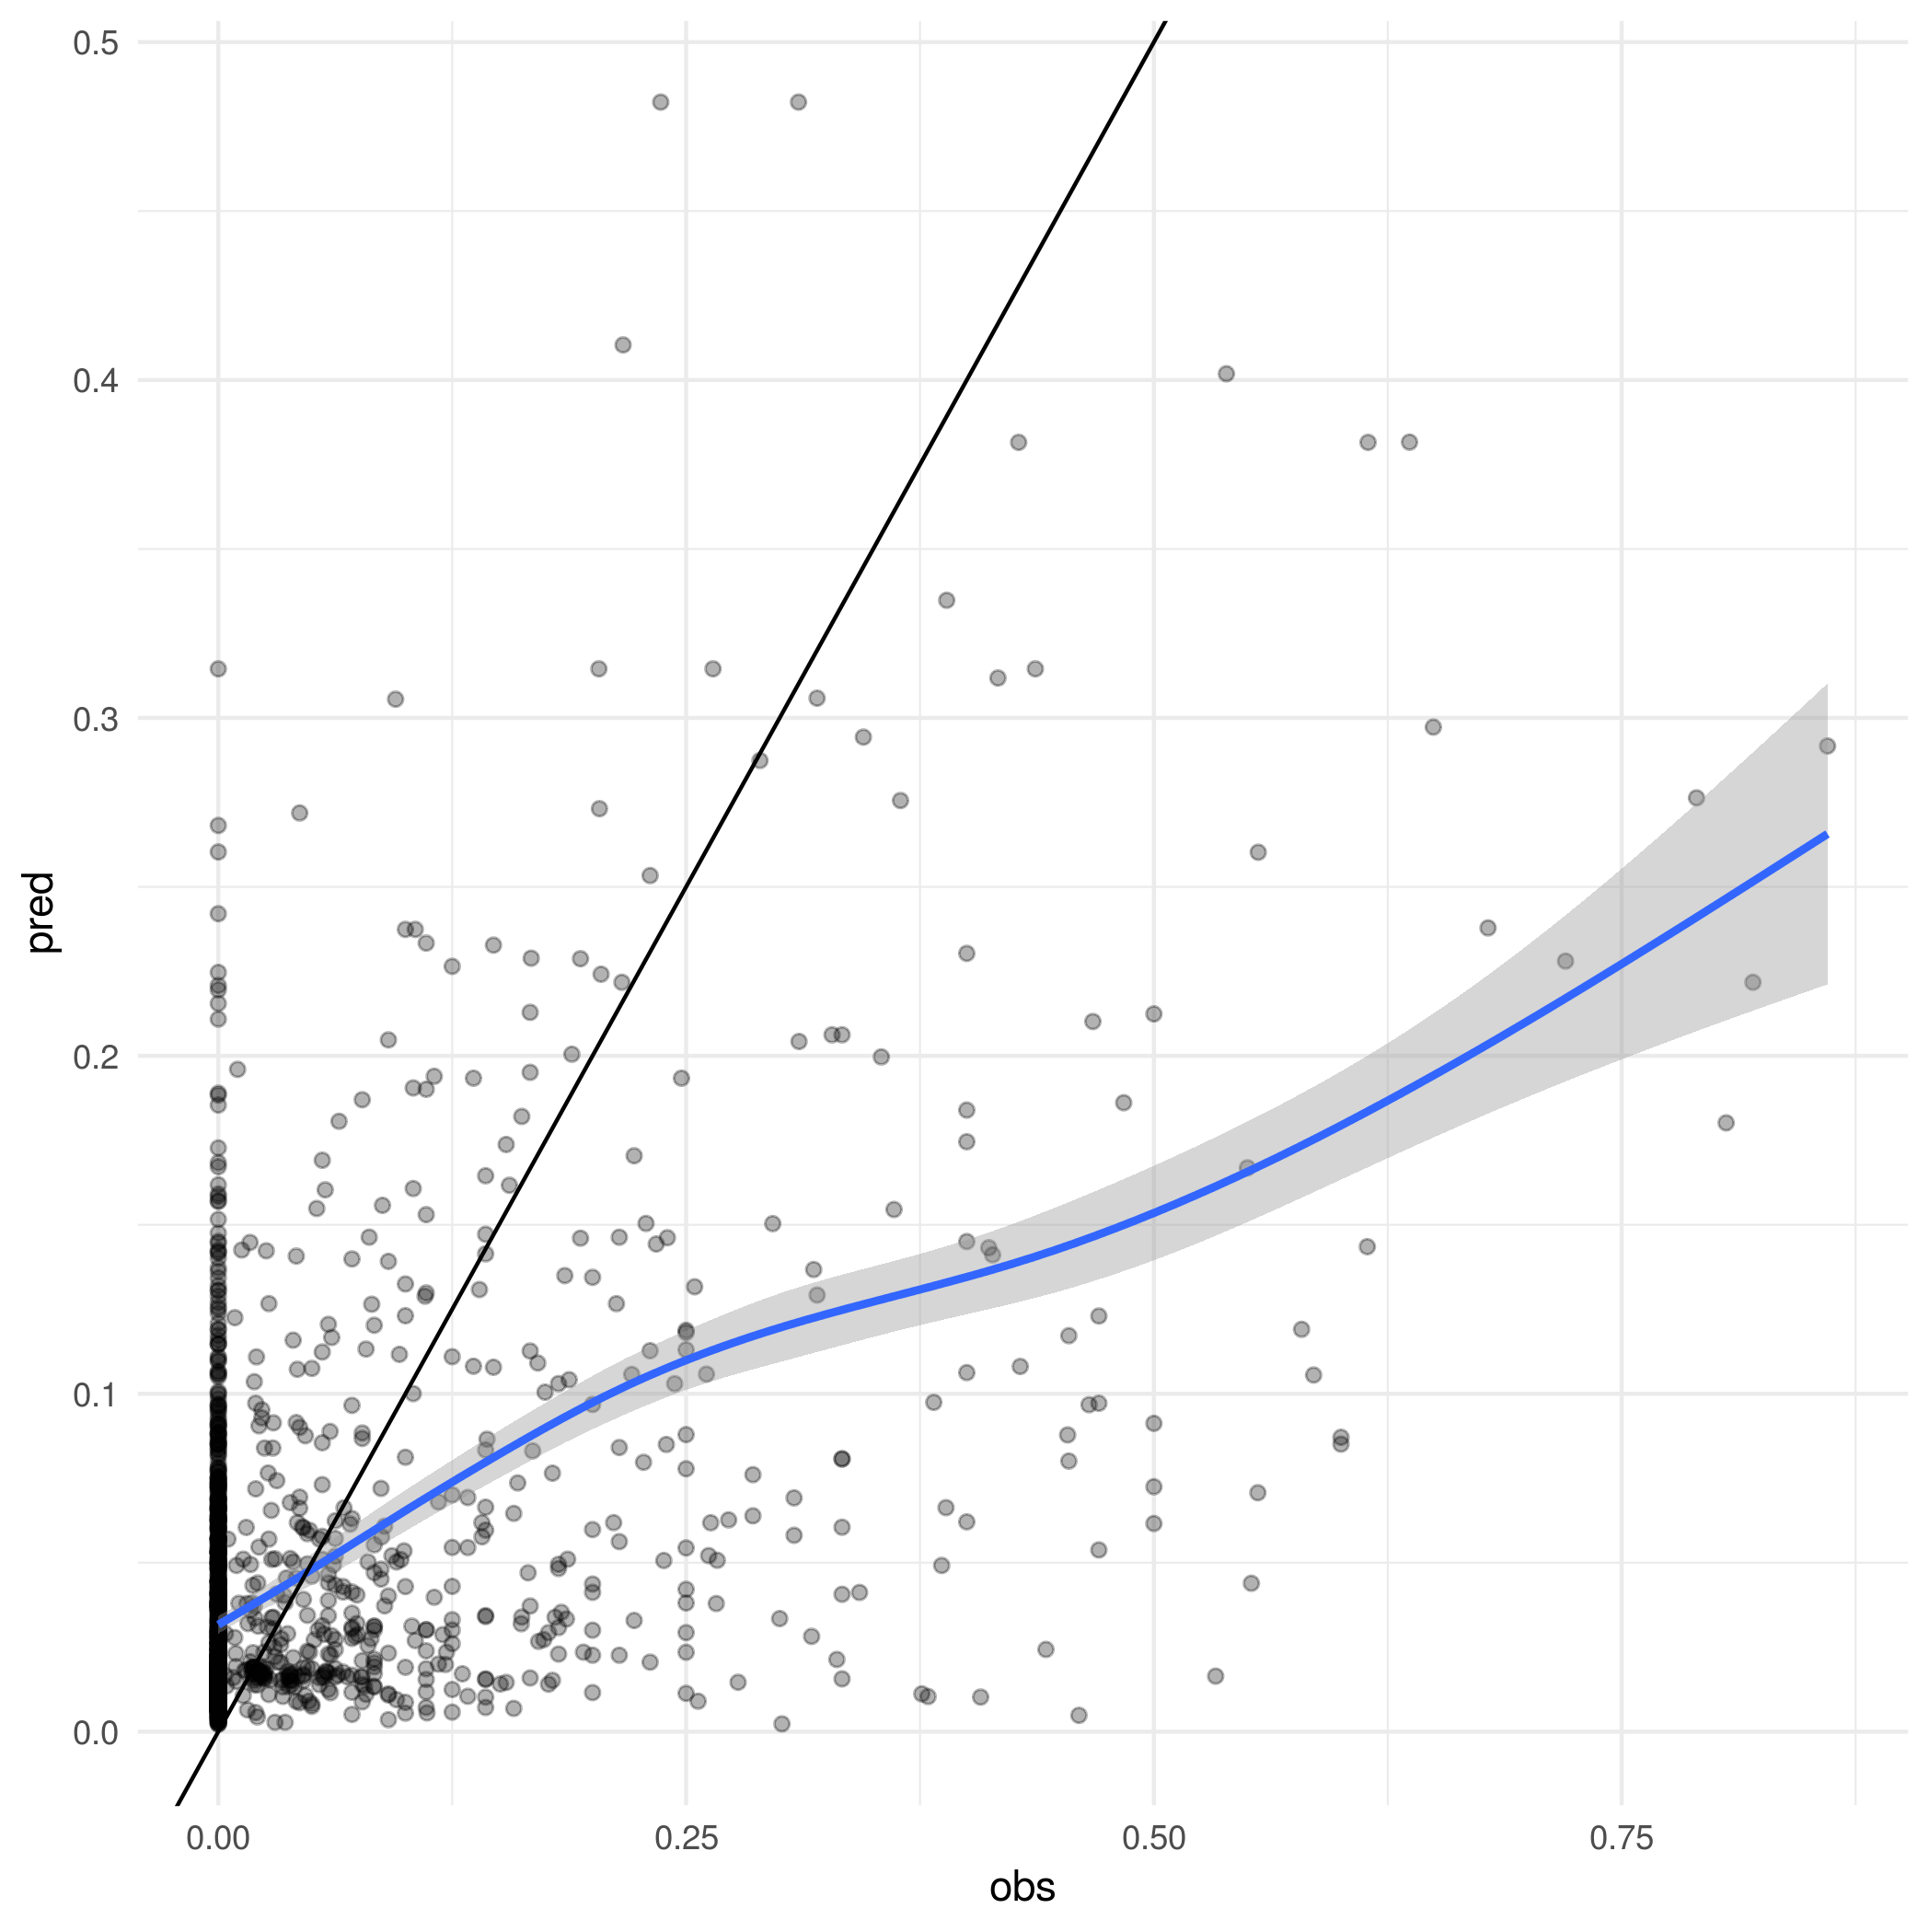
\includegraphics[width=0.6\textwidth]{figs/SI/ranger_obspred_sen.png}
\caption{
  Scatter plot of predictions and held out observed data for the Random Forest trained on the Senegal dataset.
}

\end{figure}


\begin{figure}[h!]
  \centering
  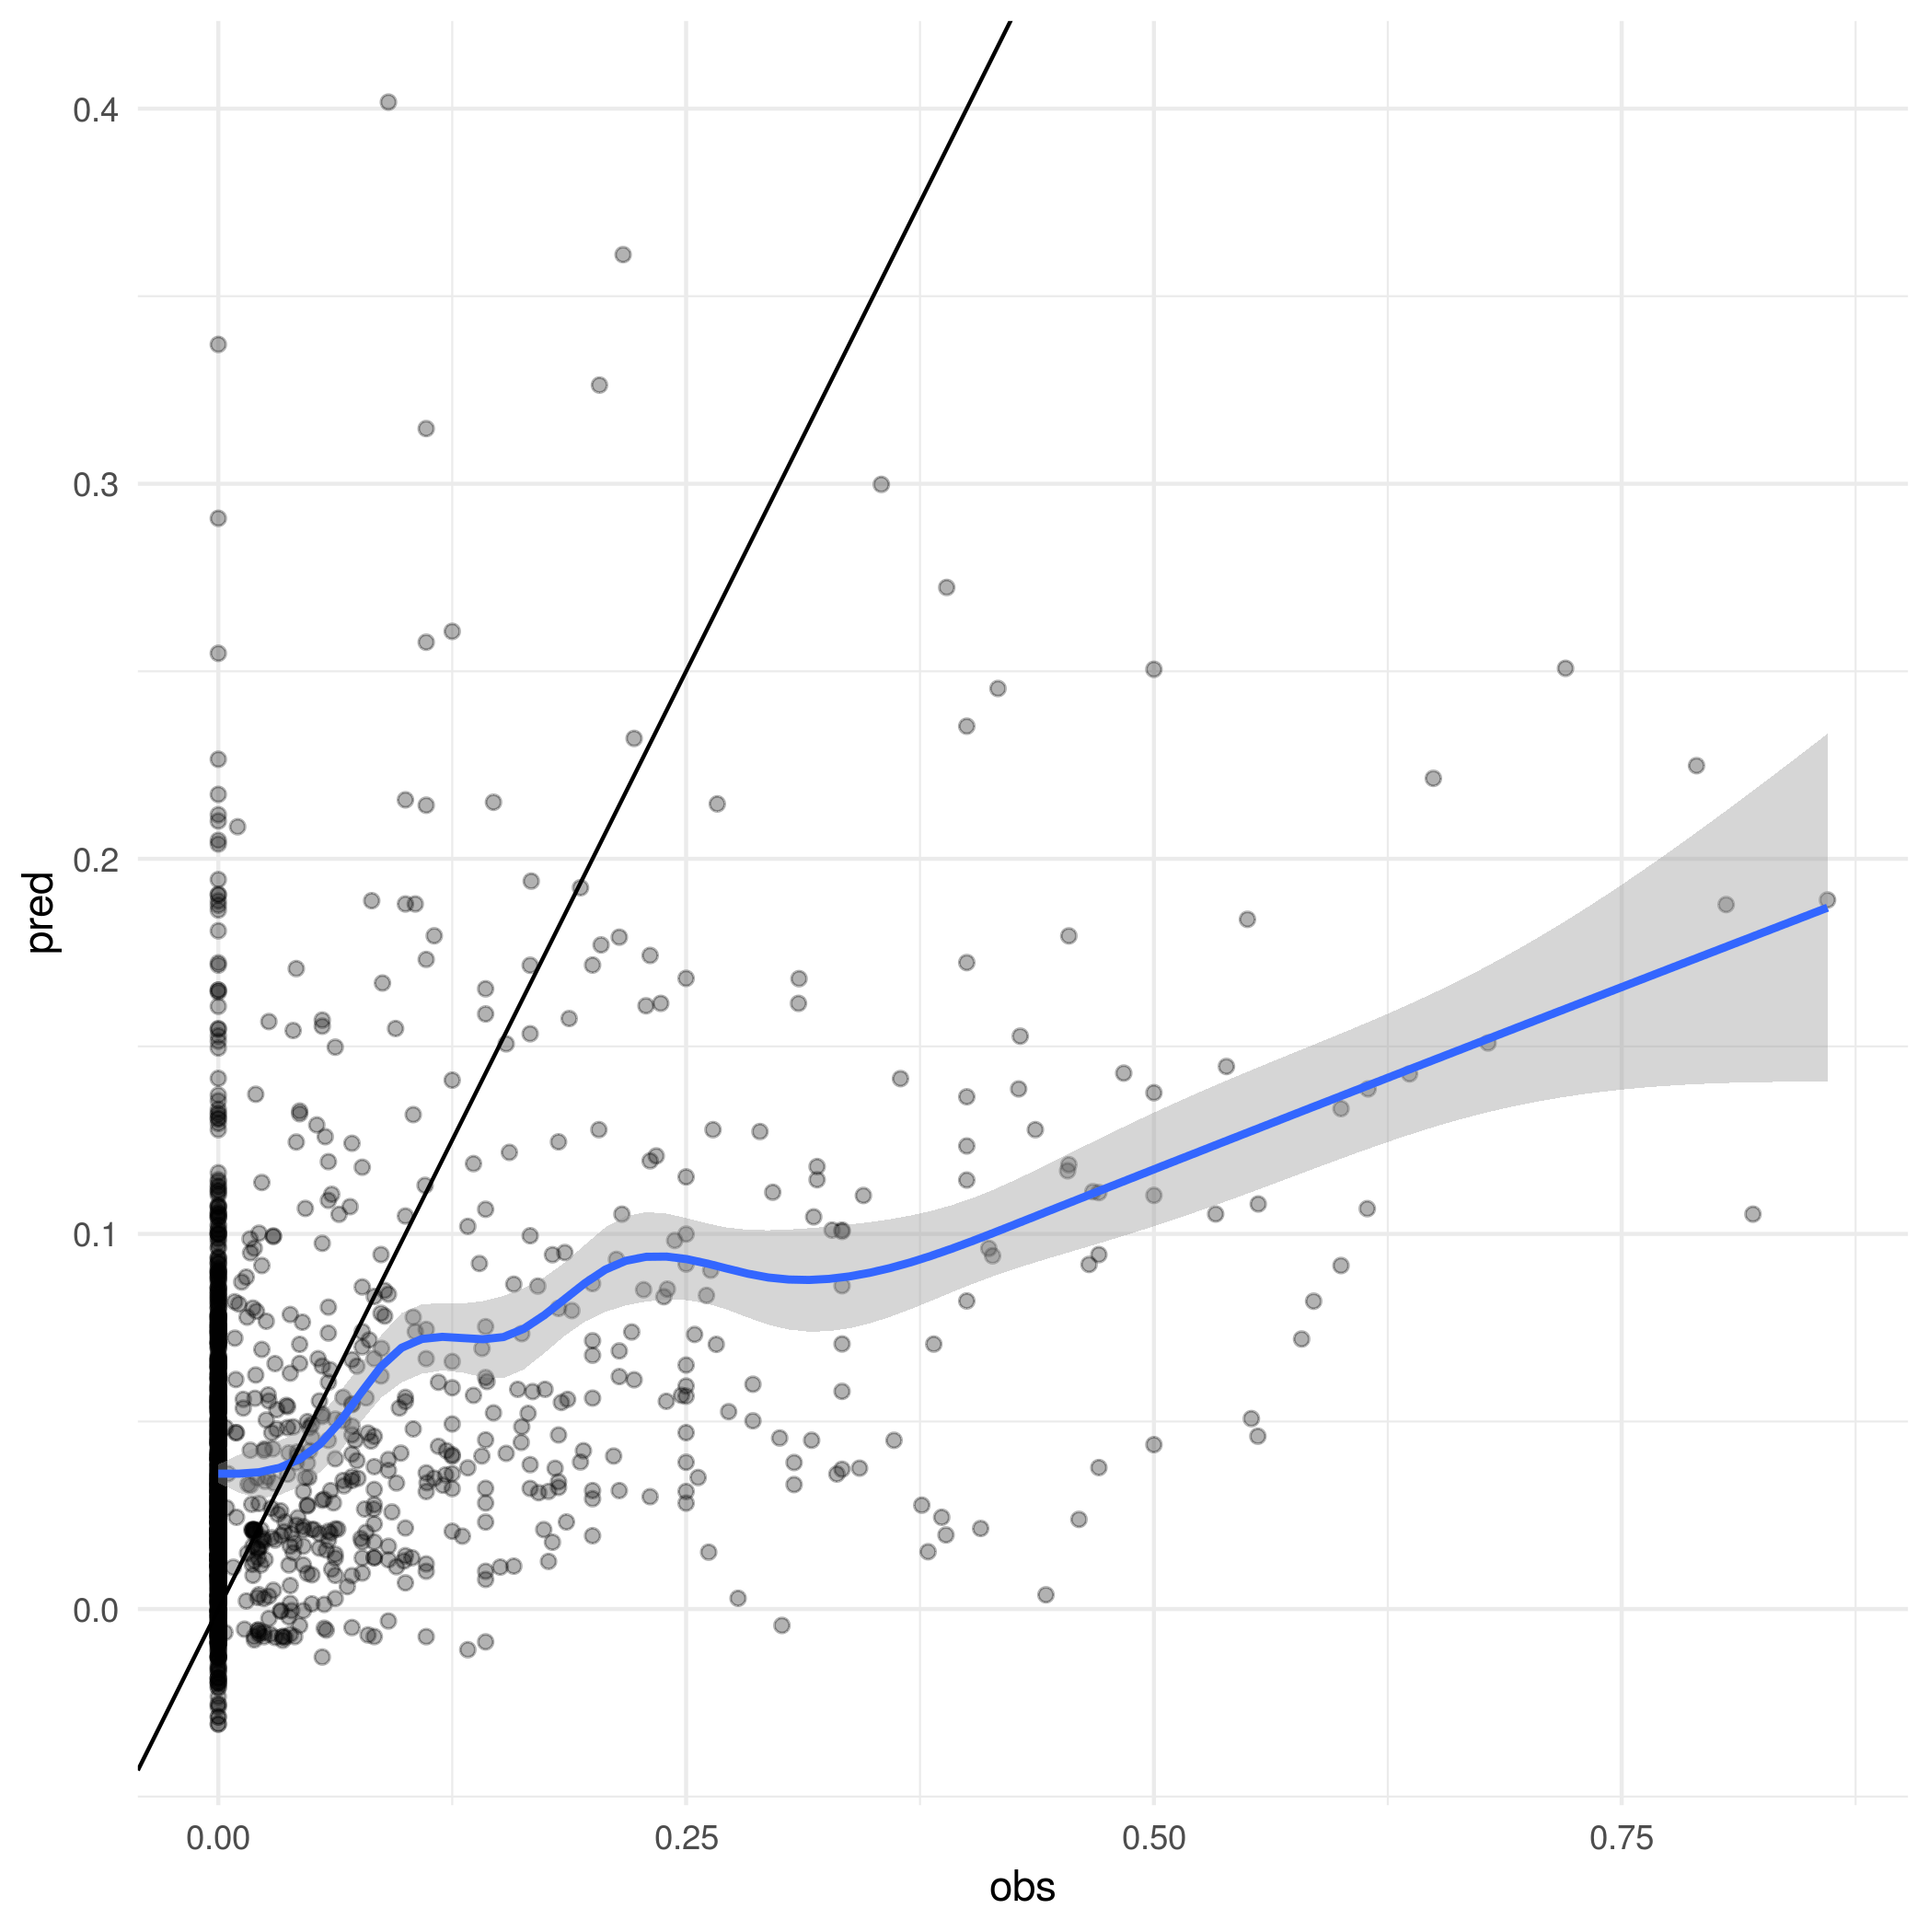
\includegraphics[width=0.6\textwidth]{figs/SI/xgboost_obspred_sen.png}
\caption{
  Scatter plot of predictions and held out observed data for the GBM trained on the Senegal dataset.
}

\end{figure}


\clearpage
\subsection{Hyperparameter optimisation}

As ranger and GBM were tuned with random hyperparameter search, the plots become difficult and are not included.


\begin{figure}[h!]
  \centering
  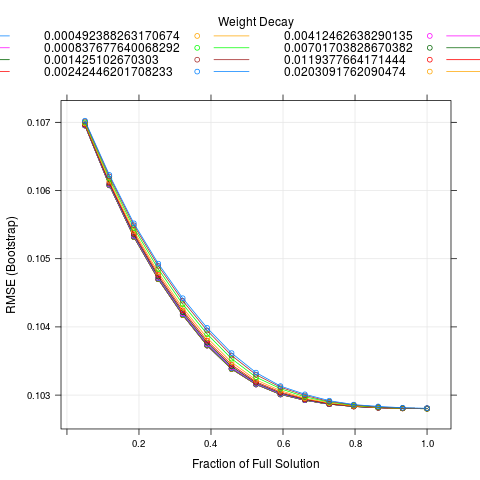
\includegraphics[width=0.6\textwidth]{figs/SI/enetopt_sen.png}
\caption{
  Optimisation for elastic net hyperparameters trained on the Senegal dataset.
}
\end{figure}



\begin{figure}[h!]
  \centering
  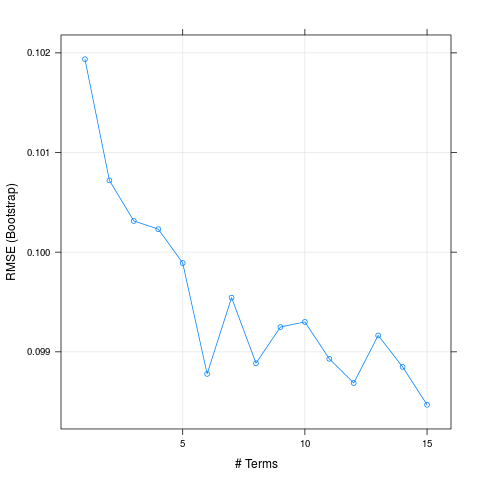
\includegraphics[width=0.6\textwidth]{figs/SI/ppropt_sen.png}
\caption{
  Optimisation for PPR hyperparameters trained on the Senegal dataset.
}

\end{figure}






\clearpage
\section{Colinearity between covariates}


\begin{figure}[h!]
  \centering
  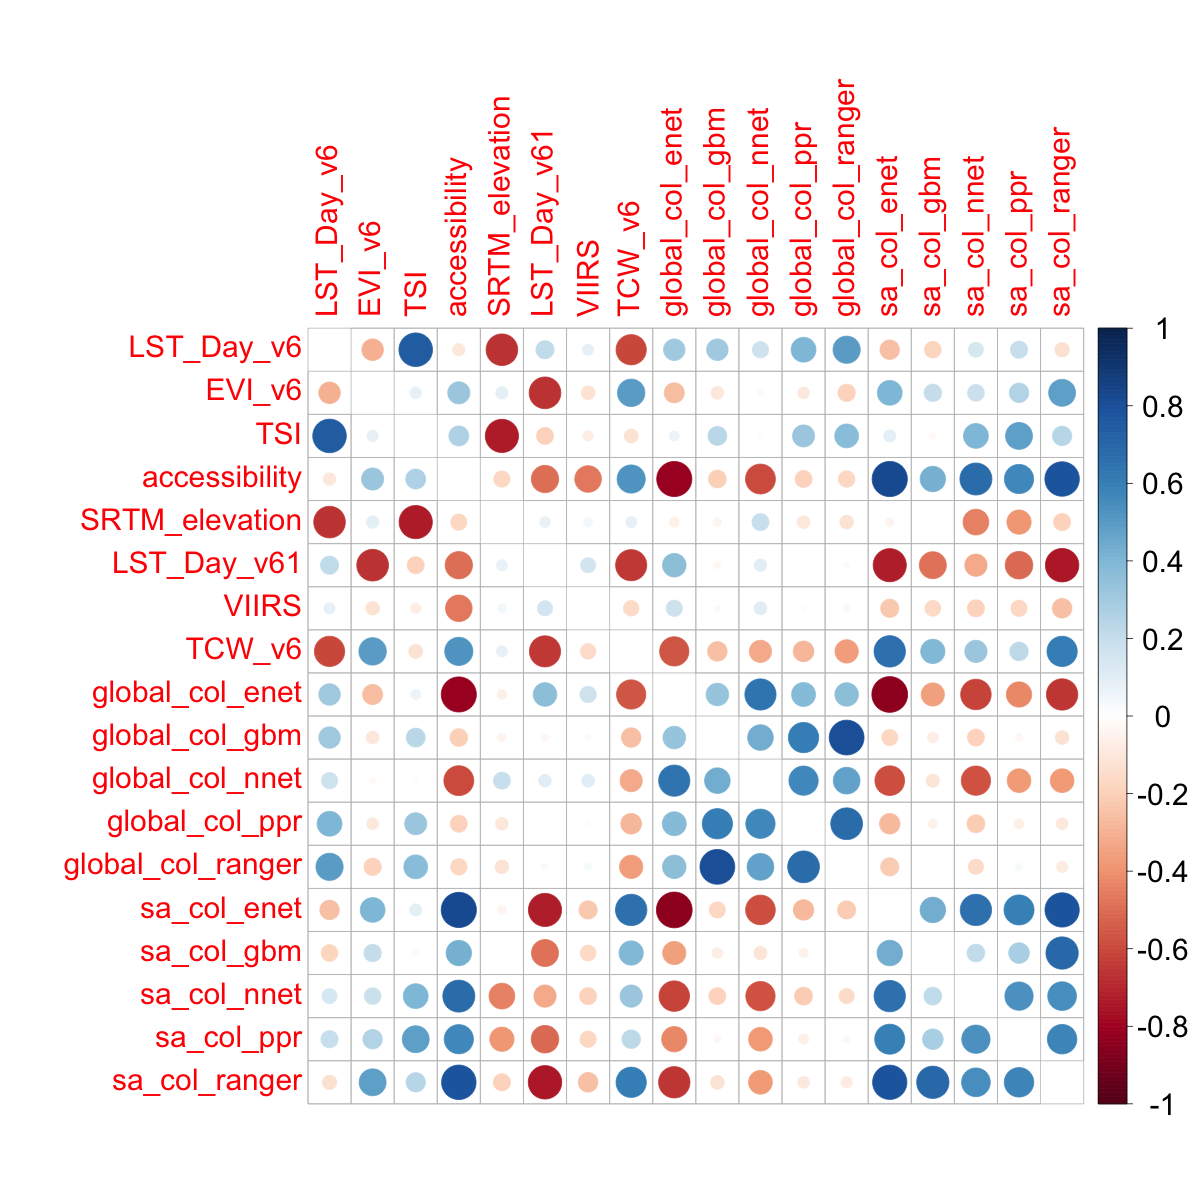
\includegraphics[width=0.7\textwidth]{figs/SI/col_correlation_plot.png}
\caption{
  Correlation matrix for all covariates (raw environmental and machine learning predictions) for Colombia}

\end{figure}


\begin{figure}[h!]
  \centering
  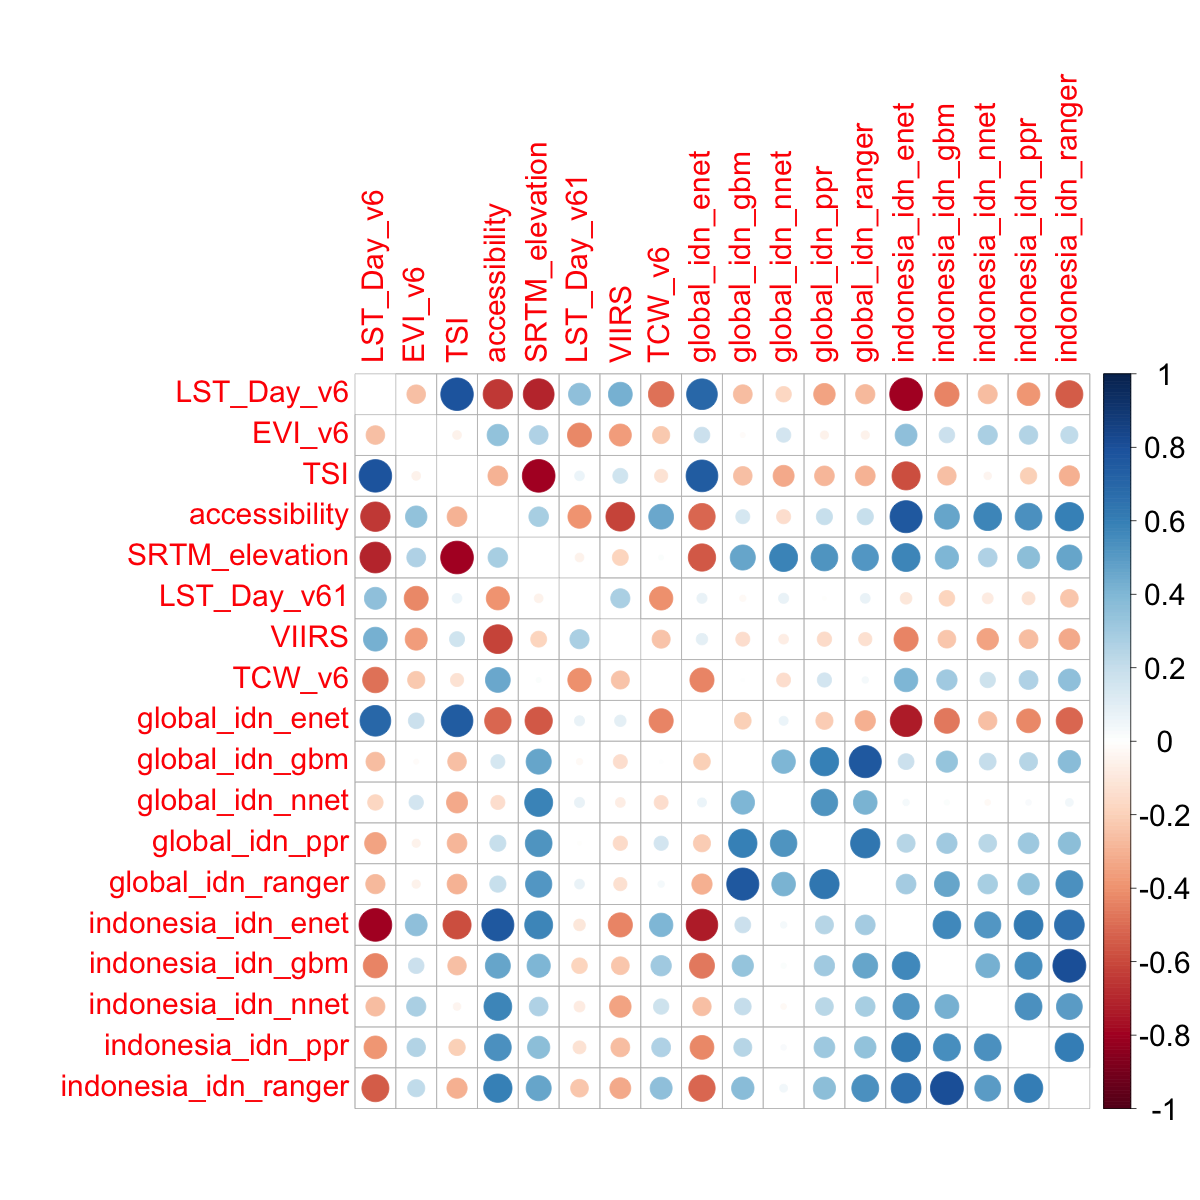
\includegraphics[width=0.7\textwidth]{figs/SI/idn_correlation_plot.png}
\caption{
  Correlation matrix for all covariates (raw environmental and machine learning predictions) for Indonesia}

\end{figure}


\begin{figure}[h!]
  \centering
  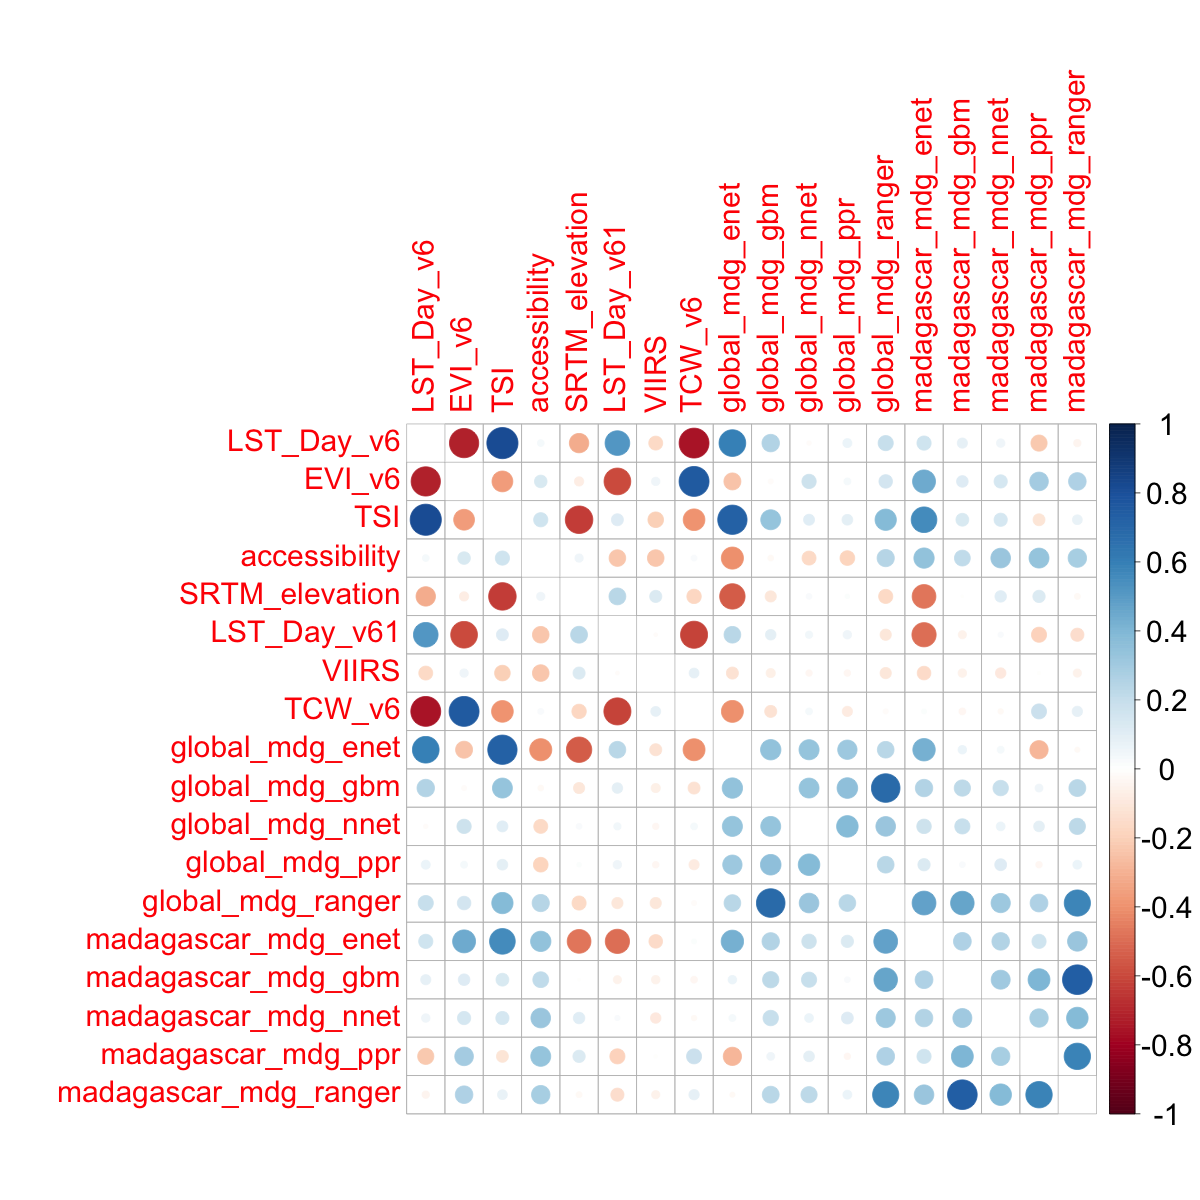
\includegraphics[width=0.7\textwidth]{figs/SI/mdg_correlation_plot.png}
\caption{
  Correlation matrix for all covariates (raw environmental and machine learning predictions) for Madagascar}

\end{figure}




\begin{figure}[h!]
  \centering
  \includegraphics[width=0.7\textwidth]{figs/SI/sen_correlation_plot.png}
\caption{
  Correlation matrix for all covariates (raw environmental and machine learning predictions) for Senegal}

\end{figure}






\clearpage
\section{Model consistency}




\begin{figure}[h!]
  \centering
  \includegraphics[width=0.9\textwidth]{figs/SI/pix_consistency_cis.png}
\caption{80\% credible interval widths for a some pixels when fitting models in Madagascar with increasing dataset sizes. The blue line is a simple linear model fit.}

\end{figure}




%\section*{Citations}
%\bibliography{Malaria} 
%\bibliographystyle{unsrt}
%\bibliographystyle{apalike}




\end{document}









